
\documentclass
[
a4paper,
german,
%twoside,
openright,                    % Kap.beginn immer rechts! (fkt. nur bei report, nicht bei article)
10pt                          % ersatzweise 12pt, wenn mehr Seiten entstehen sollen
%dvips
]
{report}
%\documentclass[a4paper,10pt]{report} %report = Diplomarbeit, article = Normal
%\usepackage[latin9]{inputenc}
%\usepackage[ngerman]{babel} 	%Deutsch
%\usepackage[T1]{fontenc}	%Deutscher Zeilenumbruch
%\usepackage{graphicx}

% ==========================================================
% Dokumentenart einstellen
% ==========================================================
%\documentclass[%
%10pt,			% 10 Pt Schriftgr??e [default]
%12pt, 			% 12 Pt Schriftgr??e
%onecolumn,	% Eine Spalte [default]
%oneside,		% Einseitiger Druck,
%twosided,		% zweiseitiger Druck, funktioniert nur bei book
%a4paper,		% Format: A4
%pdftex,			% PDF-Erzeugung erzwingen
%titlepage,		% Titelseite vorhanden
%openright		% funktioniert nur bei Report oder book
%]{report} 	% sonstige Einstellungen aus der Dokumentenart "report" verwenden

		
%\usepackage[nottoc]{tocbibind} % Literaturverzeichnis, Index, ... automatisch
															 % in die Inhaltsangabe schreiben
															 % im Normalfall muss dies mit dem Befehl
															 % \addcontentsline{toc}{chapter}{Name} geschehen
		

% ==========================================================
% Spracheinstellungen
% ==========================================================

\usepackage[ngerman]{babel}	% Silbentrennung nach neuer deutscher 
														% Rechtschreibung erm?glichen
\usepackage{bibgerm}		% Deutsches Literaturverzeichnis, nur n?tig wenn "thebibliography nicht reicht"
\usepackage{ae}					% Textsatz u.a. in Formeln optimieren
\usepackage[right]{eurosym}		% Euro Zeichen (laden erforderlich, da nicht in Standardzeichensatz vorhanden)
															% Eurozeichen recht vom Betrag wenn mit \EUR{2,49} aufgerufen sonst [left] nehmen

% ==========================================================
%% Mathematische Symbole
% ==========================================================
\usepackage{amsmath} 	% Formelsatz erm?glichen
\usepackage{amstext}	% Text in Formeln per \text{hier kommt der Text}
\usepackage{amsfonts} % f?r komplexere Formeln mit z.B. Mengensymbolen
\usepackage{amssymb}  % f?r komplexere Formeln mit z.B. Mengensymbolen
\usepackage{lscape} %Erm�glicht Querformatseiten

% ==========================================================
% Quelltext 
% ==========================================================
\usepackage{listings} % Paket f?r Syntax Highlighting in Quelltext
\lstset{
numbers=left, 			% Zeilennummerierung links
%numberstyle=\tiny, % kleine Nummern
numbersep=5pt,			% Abstand der Zeilennummerierung
breaklines=true, 		% Zeilenumbr?che erlauben
captionpos=b,			% Beschriftung unter [bottom] dem Quelltext
frame=lines, % Oberhalb und unterhalb des Listings ist eine Linie
basicstyle=\small \ttfamily, % Schriftart
keywordstyle=\color{blue}, % Farbe f�r die Keywords wie public, void, object u.s.w.
commentstyle=\color{kotzgruen}, % Farbe der Kommentare
stringstyle=\color{red}, % Farbe der Zeichenketten
numbersep=5pt,
breaklines=true, % Wordwrap a.k.a. Zeilenumbruch aktiviert
showstringspaces=false,
% emph legt Farben f�r bestimmte W�rter manuell fest
emph={double,bool,int,unsigned,char,true,false,void},
emphstyle=\color{blue},
emph={Assert,Test},
emphstyle=\color{red},
emph={[2]\using,\#define,\#ifdef,\#endif}, emphstyle={[2]\color{blue}}
} 
		
\lstset{language=C} % gew?nschte Programmiersprache, kann direkt beim Aufruf auch per
											% \begin[language=xxx]{lstlisting} gesetzt werden
											% Sprachen sind u.a. VBScript, C++, PHP, TeX, Java, SQL, XML

% ==========================================================
% Tastatur-Kodierung (PC/MAC)
% ==========================================================
%\usepackage[applemac]{inputenc}	% MAC
\usepackage[latin9]{inputenc}			% PC
\usepackage[T1]{fontenc}					% Umlaute richtige trennen

% Celsius
\usepackage{textcomp}							% Paket f?r Sonderzeichen


% ==========================================================
% Bilder, Tabellen und PDFs(einbinden)
% ==========================================================
\usepackage{graphicx}	%macht Einbinden von Bildern und Grafiken m?glich
\usepackage{float} 	% Bietet die Option H zum wirklich 
										% festen verankern von Elementen
\usepackage{rotating} % Jedes Objekt rotieren. Im Text sind dann folgende
											%  Umgebungen vorhanden:
											% \begin{sideways} % Obj. um 90? drehen
											% \begin{turn}{30} % Obj. um 30? drehen
											% \begin{rotate}{30} % wie turn aber mit mehr Abstand
											%\begin{sidewaysfigure} % gleitendes Obj. auf eigene Seite
																							% und um 90? gedreht
											% \begin{sidewaystable} % siehe sidewaysfigure
								
\usepackage{multirow}	% komplexere Tabellen erm?glichen
											% http://andrewjpage.com/index.php?/archives/43-Multirow-and-multicolumn-spanning-with-latex-tables.html
\usepackage{array}	% Macht Einbinden von Tabellen m?glich
\usepackage{floatflt} % Macht Textfluss link oder recht neben einem Bild
											% \begin{floatingfigure}[r]{0.4\textwidth}
											%	% r = Bild rechts, l = bild links
											%   \centering
											%   \includegraphics[width=0.30\textwidth]{res/meinbild.png}
											%   \caption{Das ist mein Bild}
											%   \label{fig:Mein Bild}
											% \end{floatingfigure}
																	
\usepackage{longtable} %Erm?glicht Tabellen die l?nger als eine Seite sind
\usepackage{pdfpages}	% Erm?glicht einbinden von externen PDFs

% ==========================================================
% Farben
% ==========================================================
\usepackage{color} % Eigene Farben k?nnen definiert werden
\definecolor{kotzgruen}{rgb}{0.0,0.5,0.0}
\definecolor{darkred}{rgb}{0.7,0.0,0.0}

% ==========================================================
% Sonstiges
% ==========================================================
\usepackage{pslatex}	% 'standard' PS Fonts verwenden
\usepackage{pifont} 	% spezielle Sonderzeichen erm?glichen
											% http://willbenton.com/wb-images/pifont.pdf
\usepackage{multicol} % Zum verwenden mehrerer Spalten innerhalb einer Umgebung


% ==========================================================
% Papierformat und Seitenr?der auf DIN-A4 einstellen
% ==========================================================
\usepackage{setspace}
\usepackage[paper=a4paper,left=25mm,right=25mm,top=30mm,bottom=30mm]{geometry}

% ==========================================================
% Kopfzeile: Name der Section, Fusszeile: rechtsb?ndig ``Seite von Gesamtseitenzahl''
% ==========================================================
\usepackage{fancyhdr} 			% laden des pakets
\pagestyle{fancy}			% festlegen des pagestyle
%
%%Kopf- und Fusszeilendefinition f?r normalen Flie?text
%\fancyhead{}
%\fancyfoot{}
\fancyhf{}
\lhead{\leftmark}
\rfoot{\thepage}
\renewcommand{\headrulewidth}{0.4pt} % Linie mit 0.4pt oben
\renewcommand{\footrulewidth}{0.4pt} % Linie mit 0.4pt unten

%%Kopf- und Fusszeilendefinition f?r spezielle Seiten wie z.B Chapter 
%%% Diese Seiten verwenden den Pagestyle plain, welcher nun im folgenden 
%%% ?berschrieben wird.
\fancypagestyle{plain}{%
\fancyhf{}
\lhead{\rightmark}
\rfoot{\thepage}
\renewcommand{\headrulewidth}{0.4pt} % unsichtbare Linie oben
\renewcommand{\footrulewidth}{0.4pt} % Linie mit 0.4pt unten
}

%\fancyhead{}
%\fancyfoot{}
%\lhead{\slshape \rightmark}
%\usepackage{lastpage}
%\usepackage{fancyhdr}
%\pagestyle{fancy}
%\renewcommand{\sectionmark}[1]{\markright{\thesection. #1}}
%\addtolength{\headheight}{3pt} %1
%\renewcommand{\sectionmark}[1]%
%             {\markright{\thesection\ #1}}
%\lhead[\fancyplain{}{\thepage}]%
%         {\fancyplain{}{\rightmark}}
%\rhead[\fancyplain{}{}]%
%             {\fancyplain{}{}}
%\chead[\fancyplain{}{}]%
%             {\fancyplain{}{}}
%\cfoot{} 													%Bei zweiseitigem Druck sollte 
%%\rfoot[\fancyplain{}{\rightmark}]	%das rausgenommen werden weil die Seitenzahlen
%%																		%sonst immer rechts angezeigt werden
%%             {\fancyplain{}{\thepage\ von \pageref{LastPage}}}

% ==========================================================
% Hurenkinder raus
% ==========================================================
\clubpenalty = 15000
\widowpenalty = 15000 \displaywidowpenalty = 15000

% ==========================================================
% Nach \\ und \newline nicht einr?cken
% ==========================================================
%\setlength{\parindent}{0em}

% ==========================================================
% Nummerierung bis subparagraph, Gliederung bis paragraph
% ==========================================================
\setcounter{secnumdepth}{5}
\setcounter{tocdepth}{4}

% ==========================================================
% Standardschriftart auf Helvetica/Arial (sonst Times New Roman)
% ==========================================================
\usepackage{helvet}
\renewcommand{\familydefault}{\sfdefault} % Neuladen der Schrift

% ==========================================================
% Zeilenabstand 1,5
% ==========================================================
\onehalfspacing

% ==========================================================
% Fu?noten richtig einr?cken, Zahl hochgestellt
% ==========================================================
\makeatletter
\newlength\footnoteindent
\newlength\footnotenumwidth
\newcommand*\footnotenumalign{r}
\newcommand*\footnoteformat{}

\renewcommand\footnoteformat{\textsuperscript} % Zahlen hochstellen

\setlength\footnoteindent{0.7em}%\parindent}
\settowidth\footnotenumwidth{999}%
\renewcommand\@makefntext[1]{%
	\@setpar{%
		\@@par
		\@tempdima\hsize
		\advance\@tempdima-\footnoteindent
		\parshape\@ne
		\footnoteindent\@tempdima
	}%
\parindent 1em
\par\noindent
\makebox[0pt][r]{% make everything lap into left margin
	\makebox[\footnoteindent][r]{%
		\makebox[\footnotenumwidth][\footnotenumalign]{%
			\footnoteformat{\@thefnmark}%
			}%
			\hspace*{\fill}%
		}%
	}%
	#1%
}
\makeatother

% ==========================================================
% neue Zeile nach paragraph und subparagraph
% ==========================================================
\makeatletter
\renewcommand\paragraph{\@startsection{paragraph}{4}{\z@}%
         {-3.25ex\@plus -1ex \@minus -.2ex}%
         {.5ex \@plus .2ex}%<--- Zeilenvorschub
         {\normalfont\normalsize\bfseries}}
\renewcommand\subparagraph{\@startsection{subparagraph}{4}{\z@}%
         {-3.25ex\@plus -1ex \@minus -.2ex}%
         {.5ex \@plus .2ex}%<--- Zeilenvorschub
         {\normalfont\normalsize\bfseries}}
\makeatother

% ==========================================================
% Bild- und Tabellenunterschriften links
% ==========================================================
\usepackage[nooneline]{caption2}
\makeatletter
%\captionstyle{left}
%\captionstyle{center}
\makeatother

% ==========================================================
% Index
% ==========================================================
\usepackage{makeidx}
\makeindex
% Der Index wird in TeXnicCenter per Ausgabe -> MakeIndex erstellt 
% (Dazu muss man sich im Hauptdokument befinden)
% Evtl. ist ein mehrfaches Erstellen des Dokuments n?tig

% ==========================================================
% Glossar
% ==========================================================
 \usepackage[style=super, header=none, border=none, number=none, cols=2,
 toc=true]{glossary}

 \makeglossary
 \renewcommand{\glossaryname}{Glossar} % Damit wird Glossary in Glossar umgetauft
 
% Externer Befehl. 
%(In TeXnicCenter kann dieser Befehl z.B. nach dr?cken
% von ALT +F7 im Bereich --MakeIndex als Kommando hineinkopiert werden. 
% nach Erstellung des Glossars muss dann unbedingt wieder der Standardwert "%bm" in dieses Feld eingetragen werden, da sonst die Erstellung des Indexes nicht funktioniert)

% makeindex -s DateinameOhneEndung.ist -t DateinameOhneEndung.glg -o DateinameOhneEndung.gls DateinameOhneEndung.glo

% ==========================================================
% PDF-Einstellungen (muss als letztes Paket geladen werden!)
% ==========================================================
\usepackage[
%   % Farben fuer die Links
   colorlinks=true,         % Links erhalten Farben statt Kaesten
   urlcolor=pdfurlcolor,    % \href{...}{...} external (URL)
   filecolor=pdffilecolor,  % \href{...} local file
   linkcolor=pdflinkcolor,  %\ref{...} and \pageref{...}
   citecolor=pdfcitecolor,  %Farbe von Zitaten
%   % Links
%   raiselinks=true,			 % calculate real height of the link
   breaklinks,              % Links berstehen Zeilenumbruch
   backref=page,            % Backlinks im Literaturverzeichnis (section, slide, page, none)
   pagebackref=true,        % Backlinks im Literaturverzeichnis mit Seitenangabe
%   hyperindex=true,         % backlinkex index
   linktocpage=true,        % Inhaltsverzeichnis verlinkt Seiten
%   hyperfootnotes=false,     % Keine Links auf Fussnoten
   % Bookmarks
   bookmarks=true,          % Erzeugung von Bookmarks fuer PDF-Viewer
   bookmarksopenlevel=1,    % Gliederungstiefe der Bookmarks
   bookmarksopen=true,      % Expandierte Untermenues in Bookmarks
%   bookmarksnumbered=true,  % Nummerierung der Bookmarks
%   bookmarkstype=toc,       % Art der Verzeichnisses
%   % PDF Informationen
   pdftitle={Latex-Vortrag},             % Titel
	 pdfsubject={Eine LaTeX-Einf�hrung},
   pdfauthor={Sebastian Stechl},            % Autor
]{hyperref}

% ==========================================================
% Linkfarben im PDF
% ==========================================================
% Farben fuer die Links im PDF
%\definecolor{pdfurlcolor}{rgb}{0,0,0.6}
%\definecolor{pdffilecolor}{rgb}{0.7,0,0}
%\definecolor{pdflinkcolor}{rgb}{0,0,0.6}
%\definecolor{pdfcitecolor}{rgb}{0,0,0.6}

% PDF-Linkfarben auf schwarz f?r den Druck:
 \definecolor{pdfurlcolor}{rgb}{0,0,0}
 \definecolor{pdffilecolor}{rgb}{0,0,0}
 \definecolor{pdflinkcolor}{rgb}{0,0,0}
 \definecolor{pdfcitecolor}{rgb}{0,0,0}


% ==========================================================
% Benennung von Literaturverzeichnis und Abstrakt
% ==========================================================
\addto\captionsngerman{
	\renewcommand{\abstractname}{Zusammenfassung}
	\renewcommand{\refname}{Literaturverzeichnis}
	\renewcommand{\lstlistingname}{Code}
	}

% ===========================================
% Toleranz beim Trennen erh?hen (default=200)
% ===========================================
\tolerance=1000
\newcommand{\bindestrich}{\discretionary{-}{}{-}}

% ==========================================================
% Selbstdefinierte Befehle
% ==========================================================

% Eurozeichen (als ? schreiben)
% \newcommand{\eur}{\euro\hspace{0.3em}}
\newcommand{�}{\euro} % Eurozeichen direkt eigeben
	
% ==========================================================
% ENDE DER VOREINSTELLUNGEN
% ==========================================================



\begin{document}

\pagestyle{fancy}
\begin{titlepage}
\begin{figure}
  \begin{center}
    \hbox to \hsize{%
      \begin{tabular}[m]{c}
        
\includegraphics[width=5cm]{images/fh-logo.png}
      \end{tabular}
      \hfill%
      \begin{tabular}[m]{c}
        Hochschule Augsburg\\
        Fakult�t f�r Informatik \\
	An-der-Fachhochschule 1 \\
	86161 Augsburg
      \end{tabular}%
    }
  \end{center}
\end{figure}

\begin{center}
\rule{0pt}{0pt}
\vfill
\vfill
\vfill
\vfill

\begin{huge}
Ein universelles, rekonfigurierbares und freies \\ USB-Ger�t \\ zur Timing-, Protokoll-, Logik- und Eventanalyse \\ von digitalen Signalen \\
\end{huge}

\vfill
\vfill

Bachelorarbeit im Studiengang Technische Informatik\\ von\\

\vspace*{.5cm}
Andreas M�ller\\
geboren am: 27.07.1982\\
Martrikelnummer: 912440\\
\vspace{.5cm}
11. Juni 2010 \\

\vfill
\vfill
\vfill
\vfill

\begin{tabular}{rl}
Erstpr�fer: Prof. Dr. Hubert H�gl\\
Zweitpr�fer: Prof. Dr. Gundolf Kiefer\\

\end{tabular}
\end{center}
\end{titlepage}



\newpage

\text{ }

\noindent
\textbf{Danksagung}

\vspace{1cm}

\noindent
Diese Diplomarbeit entstand an der Fakult�t f�r Informatik der Hochschule Augsburg, unter der Leitung von Herrn Prof. Dr. Hubert H�gl. Besonders m�chte ich mich bei Herrn H�gl f�r die M�glichkeit bedanken, diese Bachelorarbeit anfertigen zu d�rfen.

\noindent
Auch m�chte ich mich bei Prof Dr. Gundolf Kiefer bedanken, der mir bei Fragen zum Logikentwurf zur Seite stand, auch wenn dies nicht mehr verwirklicht wurde.

\noindent
Au�erdem gilt mein Dank Marcus Stegner und Michael Sch�ferling die mir, als Mitarbeiter des Labors f�r Technische Informatik, immer in bei allen Soft- und Hardwareproblemen geholfen haben und mich mit Ihrer Laborausstattung sehr unterst�tzten.

\noindent
Auch danke ich meinem Komilitonen Florian Richter, der mich in den hektischen Zeiten w�hrend des Verfassens dieser Arbeit, immer moralisch und mit viel Kaffee unterst�tzte.

\noindent
Bei meiner Mutter m�chte ich mich ganz herzlich f�r das, sicherlich sehr anstrengende, Korrekturlesen einer technischen Abschlussarbeit bedanken. Auch danke ich meiner ganzen Familie f�r die finazielle Unterst�tzung der vergangenen sieben Jahre an der Hochschule Augsburg und des unvergesslichen Auslandsemesters in Schweden.

\vspace{3cm}

\noindent
\textbf{Erstellungserkl�rung}

\vspace{1cm}

\noindent
Andreas M�ller\\
Wertachbrucker-Tor-Str. 9\\
86152 Augsburg

\vspace{1cm}

\noindent
Ich versichere, dass ich die Arbeit ohne fremde Hilfe und ohne Benutzung anderer als der
angegebenen Quellen angefertigt habe und dass die Arbeit in gleicher oder �hnlicher Form noch
keiner anderen Pr�fungsbeh�rde vorgelegen hat und von dieser als Teil einer Pr�fungsleistung
angenommen wurde. Alle Ausf�hrungen, die w�rtlich oder sinngem�� �bernommen wurden, sind
als solche gekennzeichnet.

\vspace{2cm}

\noindent
Augsburg, den 11. Juni 2010\\
\medskip
\medskip

\noindent
\underline{~~~~~~~~~~~~~~~~~~~~~~~~~~~~~~~~~~~~~~~~}\\
Andreas M�ller\\



\newpage



\begin{abstract} % Zusammenfassung

\noindent
Diese Arbeit handelt von der Entwicklung der Plattform f�r ein universelles, rekonfigurierbares und freies USB Ger�t, zur Timing-, Protokoll-, Logik- und Eventanalyse von digitalen Signalen.

\noindent
Hauptaufgabe des Ger�tes ist es, exakte Timing-Analysen an Mikrocontrollern oder �hnlichem durchzuf�hren. So kann zum Beispiel die Dauer eines Prozesses extern gemessen werden, ohne dass durch die Messung die Laufzeit beeinflusst wird.

\noindent
Kerst�ck des Systems ist ein konfigurierbarer Logikbaustein (CPLD) der Firma Altera, sowie ein Mikrocontroller der Firma Atmel mit USB Anbindung.

\noindent
Das gesamte Projekt, sowohl Hard- als auch Software, ist im Sinne von Open-Source frei verf�gbar und kann unter der URL

\begin{center}
\begin{large}
\url{http://sta.informatik.fh-augsburg.de}
\end{large}
\end{center}

\noindent
abgerufen werden. Auch ein SVN Repository mit TRAC ist unter dieser Adresse verf�gbar.

\end{abstract}

\tableofcontents

%Hier gehts los:
\chapter{Einf�hrung} % Kapitel 1

\section{Motivation} \label{Motivation}

Digitale Schaltungen und Mikroprozessoren befinden sich heutzutage in so gut wie jedem Ger�t. Die Bandbreite geht hier von einfachen Kaffemaschinen, bis hin zur komplexen Automatiserungstechnik zum Beispiel einer Autowaschstra�e.

Hierf�r sind auch zeitlich miteinander abgestimmte Prozesse und Echtzeitanwendungen n�tig. So l�st zum Beispiel ein Sensor, wie eine Lichtschranke, einen Interrupt-Subroutine innerhalb eines Mikrocontrollers aus. Dieser springt nun aus seinem Hauptprogramm in das entsprechende Unterprogramm. Nun ist es f�r den problemlosen Ablauf einer Steuerung manchmal wichtig, schon vor Ausf�hrung des Unterprogramms zu wissen, wie lange die Ausf�hrung vermutlich dauern wird.

Dies kann nur durch ein vorheriges messen der Dauer erfolgen. Diese Messung kann nun nat�rlich von der Anwendung selbst erfolgen. Jedoch muss hier beachtet werden, dass die Funktion zur Zeitmessung ebenfalls Ausf�hrungszeit ben�tigt, was das Ergebnis, welches im Millisekunden-Bereich liegen kann, verf�lscht. 

Als weiteres kommt noch eine externe Messung in Frage. Daf�r wird zu Beginn und Ende der zu messenden Funktion ein Hardwarpin gesetzt. Dieses Setzen eines Hardwarpins verf�lscht bei modernen Mikrocontrollern das Ergebnis maximal um einen Takt. Nun kann dieses Signal durch ein externes Ger�t registriert werden, und die Zeit zwischen den beiden Pulsen gemessen werden. 

Ein solches Ger�t m�sste mindestens �ber einen Messleitungs-Eingang, einen Zeitgeber und einen Zwischenspeicher verf�gen. Auch ein Ausgang zur Datenanalyse muss vorhanden sein.

\section{Ziel der Arbeit}

Ziel der Arbeit ist es, eine Basis f�r den oben erw�hnen Analysator zu schaffen. Dazu geh�ren die Auswahl der Komponenten, das Erstellen des Schaltplanes und das Fertigen und Testen des Prototypen.

Auf Softwareseite sollen M�glichkeiten aufgezeigt werden, wie mit dem Ger�t kommuniziert werden kann. Dazu geh�ren die Implementierung einer USB-Schnittstelle f�r die Kommunikation mit der Hardware. Ausserdem soll �ber die selbe Schnittstelle ein Austausch der Firmware erfolgen k�nnen.

Ein komplett funktionsf�higer Analysator wurde in dieser Arbeit nicht erstellt. Jedoch wird eine m�gliche Implementierung sowohl auf Softwareseite als auch auf Seite der logischen Schaltung erl�utert.

Auf der so erstellten Basis, kann nun in zuk�nftigen Arbeiten oder Projektgruppen ein Analysator entwickelt werden, der die unter Abschnitt \ref{Motivation} erw�hnten Funktionen erm�glicht. Auch sind durch die Flexibilit�t des verwendeten Mikrocontrollers und des Logikbausteins eine Vielzahl weiterer Funktionen m�glich.

\section{Open-Source}

Die gesamte Arbeit steht unter einer Open-Source Lizenz. Dies betrifft zum einen die Software, also die Firmware des Mikrocontrollers, den VHDL-Code des Logikbausteins und die PC-Software. Au�erdem steht die Hardware, also die Schaltpl�ne und das Platinenlayout, auch unter einer Open-Hardware-Lizenz.

Als Lizenz wurde die LGPL-Lizenz ausgew�hlt. Diese Lizenz erlaubt es auch komerziellen Anwendern die Soft- und Hardware in Ihre Anwendungen zu Integrieren. Eine genaue Beschreibung der Lizenz befindet sich im Anhang. Einige der verwendeten Codeabschnitte und Programme verf�gen �ber eine eigene Lizenz. Der Hinweis auf diese Lizenzen befindet sich in den entsprechenden Quellcode-Dateien. 

F�r den schriftlichen Teil der Bachelorarbeit wurde die GNU-Lizenz f�r freie Dokumentation ausgew�hlt, was sowohl nichtkommerzielles als auch kommerzielles Kopieren ausdr�cklich erlaubt.

\begin{center}

\includegraphics[width=0.3\textwidth]{images/lgpl.png}
\end{center}

\section{Aufbau der Arbeit}

In Kapitel 2 wird die Theorie der digitalen Messtechnik angeschnitten. In den Kapiteln 3 und 4 wird die Entwicklung des Hardwareprototypen erl�utert. Die Kapitel 5 bis 7 befassen sich mit der Firmware des Mikrocontrollers. Die PC-Software wird in Kapitel 8 und da VHDL-Desighn in Kapitel 9 erkl�rt. 

Ein Ausblick auf die zuk�nftige Entwicklung befindet sich unter Kapitel 10. Im Anhang sind Schaltpl�ne, Listen und Verzeichnisse sowie die LGPL-Lizenz abgedruckt.
\chapter{Digitale Messtechnik} % Kapitel 2

\section{Einf�hrung} \index{Digitale Messtechnik} \index{Messtechnik}

Die digitale Messtechnik steht als Oberbegriff f�r jegliche Messverfahren, welche nicht aus rein analogen oder mechanischen Komponenten aufgebaut sind. Es ist jedoch nicht davon auszugehen, dass es sich immer um eine komplett digitalisierte L�sung handelt. Bei einem Gro�teil der Messverfahren geschieht die Aufbereitung, wie zum Beispiel die Verst�rkung oder Filterung eines elektrischen Signals, mittels einer analogen Schaltung. Dieses Signal wird dann durch ein geeignetes Verfahren digitalisiert und kann nun durch digitale Schaltungen oder einen PC-Messplatz weiterverarbeitet und dargestellt werden. Der wichtigste Grundsatz in der digitalen Messtechnik ist das Abtasttheorem von Claude Shannon und W. A. Kotelnikov. Dies besagt, dass die Abtastfrequenz $f_{a}$ der Messung mindestens doppelt so gro� sein muss als die maximale Frequenz des zu messenden Signals $f_{max}$. \cite{Hoffm02}

\begin{quote}
$f_{a} > 2 f_{max}$ 
\end{quote}

In der Praxis jedoch wird, zur Vermeidung gr��erer Messfehler bei der Amplitudenmessung, �blicherweise eine Abtastfreqenz von $f_{a} = (5...10) f_{max}$ verwendet.

\section{Speichergest�tzte Messtechnik} \index{Speichergest�zte Messtechnik}

Ein gro�er Nachteil der analogen Messtechnik ist die stark begrenzte Speicherm�glichkeit analoger Signale. Diese erfolgt meist nur in einem stark begrenzten Zeitbereich zum Beispiel durch das Nachleuchten einer braunschen R�hre in einem Osziloskop. Dauerhafte Speicherung ist hier meist nur durch aufwendige Verfahren, wie das Belichten eines Fotopapiers, m�glich.
Hier liegt nun ein gro�er Vorteil bei der digitalen Messtechnik. Messwerte, welche in digitaler Form vorliegen, k�nnen verlustfrei in fl�chtigen oder nicht-fl�chtigen Speichern abgelegt werden um zu einem sp�teren Zeitpunkt weiterverarbeitet oder dargestellt zu werden. Auch k�nnen die Messwerte so mit verschiedenen Analyseverfahren, wie zum Beispiel einer Fourier-Transformation, aufbereitet werden ohne dabei an Qualit�t zu verlieren. Durch die heutzutage verf�gbaren g�nstigen Speicherbausteine mit hoher Datendichte ist es problemlos m�glich Messignale �ber einen gro�en Zeitraum zu speichern, um sie sp�ter weiterverarbeiten zu k�nnen. Auch k�nnen die Messwerte �ber eine Datenverbindung zu einem beliebigen, vom Messplatz unabh�ngigen, Ort zur Verarbeitung �bertragen werden.

Worauf jedoch bei der speichergest�tzten Messtechnik geachtet werden muss ist die Schreibgeschwindigkeit der Speicherbausteine bzw. die Geschwindigkeit des verwendeten Bussystems. Diese muss so ausgelegt sein, dass, bei gleicher Gr��e des Datenwortes, die Speicherzugriffszeit kleiner oder gleich ist der Abtastzeit des Messsignals.

\begin{quote}
$T_{Speicher} \leq T{a}$ 
\end{quote}

\section{Messignale} \index{Messignale} \index{Komparator} \index{Schmitt-Trigger}

Im Gegensatz zur Digitalisierung von kontinuierlichen analogen Signalen, welche relativ aufwendige Schaltungen ben�tigt, ist die Erfassung von bereits digitalen Messsignalen relativ einfach aufgebaut. Da in dieser Arbeit nur mit Signalen gearbeitet wird, welche die Zust�nde \textit{High} und \textit{Low} besitzen, kann auf eine Digitalisierung der Signale durch einen Analog/Digital-Wandler verzichtet werden. Stattdessen wird ein einfacher Komparator oder Schmitt-Trigger verwendet, um die vorliegenden Signalpegel in digitale Messwerte zu wandeln.

Bei einem einfachen Komparator, welcher in der Grundschaltung nur aus einem Operationsverst�rker besteht, geht das Ausgangssignal beim �berschreiten eines bestimmten Schwellwertes $V_{ref}$, von $V_{max}$ (logisch 1) auf 0V (logisch 0) zur�ck. Dadurch wird ein negiertes, jedoch rein digitales Signal ohne Amplitudenfluktuation erzeugt. Dieses Signal kann nun von einer digitalen Schaltung weiterverarbeitet und gespeichert werden.

\begin{figure}[ht]
%Grafik �hnlich PC Messtechnik Sewite 149
	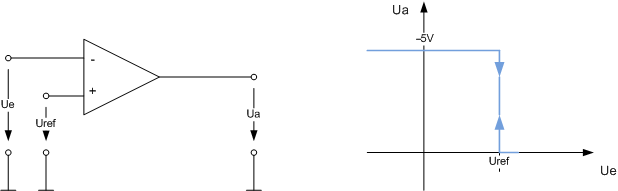
\includegraphics[width=1.0\textwidth]{images/Komparator.png}\\
	\rule{\linewidth}{0.5pt}
	\caption{Komparator mit Kennlinie}
\end{figure}

Der gro�e Nachteil des Komparators ist jedoch, dass bei einer Amplitudenfluktuation um den Schwellwert ein ungew�nschtes Prellen des Ausganssignals verursacht wird. Dieses Prellen verursacht einen mehrfachen Wechsel des Messwertes innerhalb eines Zeitraumes, in dem das zu messende Signal eigentlich einen relativ konstanten Pegel besitzt. Um diese starke Verf�lschung der Messung zu verhindern, kann ein Schmitt-Trigger eingesetzt werden.

Der Schmitt-Trigger besitzt im gegensatz zum Komparator zwei Schwellwerte um das Signal zu digitalisieren. Der erste Schwellwert liegt etwas �ber der gew�nschen Referenzspannung und veranlasst den Schmitt-Trigger das Ausganssignal auf logisch 0 zu setzen. In der Grundbeschaltung des Schmitt-Triggers liegt der Pegel des Ausganssignales hier bei etwa der negativen Versorgungsspannung $-U_{V}$. Wird dieser Schwellwert nun wieder unterschritten, so bleibt der Schmitt-Trigger in seinem Zustand. Dies wird durch eine Mitkopplung des Ausgangssignals am Plus-Eingang des Operationsverst�rkers bewrikt, welche den Schwellwert auf eine Spannung etwas unter der Referenzspannung absenkt. Erst wenn dieser, tiefer liegende, zweite Schwellwert unterschritten wird, wird das Ausgangssignal wieder auf logisch 1 ($+U_{V}$) gesetzt.

\begin{figure}[ht]
%Grafik �hnlich PC Messtechnik Sewite 149
	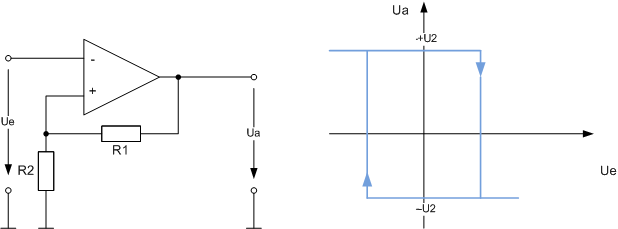
\includegraphics[width=1.0\textwidth]{images/Schmittrigger.png}\\
	\rule{\linewidth}{0.5pt}
	\caption{Schmitt-Trigger mit Hysteresekurve}
\end{figure}

Durch die so entstehende Hysterese wird ein Prellen des Ausgangssignal verhindert. Dadurch wird eine Verf�lschung der Messung durch St�rgr��en um den Schwellwert vermieden. Jedoch ist bei beiden Methoden darauf zu achten, dass das Ausgangssignal negiert ist. Dies kann jedoch in der nachfolgenden digitalen Schaltung zum Beispiel durch ein logisches \textit{NOT} korrigiert werden. \cite{Schwe97} In dieser Arbeit ist der Schmitt-Trigger bereits in dem verwendeten CPLD integriert, welcher im Abschnitt \nameref{Logikbaustein} n�her erl�utert wird.


\section{Erfassung von Zeitgr��en} \index{Zeitgr��e} \index{Oszillator} \index{Z�hler} \index{Zeitstempel}

Bei der Analyse von digitalen Signalen ist die Messung der Amplitude normalerweise zweitrangig und wird haupts�chlich zur Bestimmung der Signalqualit�t verwendent. Ein wesentlich wichtigeres Merkmal ist der Zeitpunkt wann ein Signal einen Zustandswechsel erf�hrt oder die Dauer eines bestimmten Signalzustandes. 

Um dies zu erm�glichen, muss eine m�glichst genaue Referenzzeit erzeugt werden auf deren Basis alle Messungen von Pulsdauer oder -zeitpunkt erfolgen. Dazu verwendet man in den meisten F�llen einen hochgenauen Frequenzgenerator mit fixer Periodendauer, einen sogenannten Oszillator. Diese Oszillatoren sind f�r g�ngige Frequenzen zu relativ niedrigen Preisen und einer hohen Genauigkeit von $\pm$ einigen ppm \footnote{parts per million dt.: millionstel} erh�ltlich.

Auf dieser Zeitbasis aufbauend kann nun in Kombination mit einem Z�hler eine Zeitmessung stattfinden. Dazu wird der Z�hler zum Beginn eines Ereignisses auf 0 gesetzt und der Impuls des Oszillators �ber ein Gate an den Pulseingang des Z�hlers geschaltet. Ist das Ereignis vorbei, schlie�t sich das Gate wieder und der Z�hler stoppt. Nun entspricht der Z�hlerstand der Anzahl der in diesem Zeitraum erzeugten Pulse des Oszillators. Nun kann mit der Formel

\begin{quote}
$T = N \cdot \bigtriangleup t$
\end{quote}

die gemessene Zeit $T$ berechnet werden. Wobei $N$ f�r den Z�hlerstand und $ \bigtriangleup t$ f�r die Zeitbasis steht. \cite{Schwe97} 

Eine weitere M�glichkeit der Zeiterfassung ist es, nicht den absoluten Z�hlerstand nach Ablauf des Ereignisses zu verwenden, sondern die Differenz der Z�hlerst�nde zwischen zwei Ereignissen.

\begin{quote}
$T = (N_{b} - N_{a}) \cdot \bigtriangleup t$
\end{quote}

Dies hat mehrere Vorteile. Zum Einen muss der Z�hler nicht nach jedem Ereignis zur�ckgesetzt werden. Da dieses R�cksetzten eventuell l�nger dauert als eine Zeiteinheit, kann dadurch das Messergebnis verf�lscht werden. Auch k�nnen so mehrere Ereignisse leichter in Relation zueinander gesetzt werden. So kann man sehr leicht den Zeitraum zwischen Ereignis 3 und Ereignis 5 bestimmen, ohne vorher die Zeitr�ume zwichen Ereignis 3 und 4 oder 4 und 5 zu kennen. 

Realisiert wird diese Methode der Zeiterfassung, indem man jedes Ereignis mit einem sogenannten Zeitstempel versieht. Das bedeuted, dass jedem Ereignis der zu diesem Zeitpunkt aktuelle Z�hlerstand zugeordnet wird. Diese Methode wird auch bei dieser Arbeit angewendet und im Kapitel \nameref{VHDL-Design} n�her erl�utert. 

\section{Logikanalyse} \index{Logikanalyse} 

Kombiniert man die Erfassung der Messsignale mit der Zeiterfassung, so kann auf dieser Basis eine Logikanalyse durchgef�hrt werden.

Bei einer Logikanalyse werden logische Zust�nde von mindestens einem Signal als Funktion der Zeit erfasst. Meist werden jedoch mehrere Signale von mindestens 16 Kan�len aufgezeichnet, um so zum Beispiel die verschiedenen Datenleitungen eines Bussystems als Funktion der Zeit darstellen zu k�nnen. Hierbei ist noch auf zwei unterschiedliche Messverfahren zu achten: Die synchrone und die asynchrone Signalanalyse.

Bei der synchronen Signalanalyse wird das Eingangssignal auf ein bestimmtes Taksignal einsynchronisiert. Dazu wird das Eingangssignal zun�chst in einem Register zwischengespeichert. Eine oder mehrere Eingangleitungen werden zu einem Trigger geleitet. Dieser Trigger reagiert auf eine bestimmte Signalkombination und gibt ein Ausganssignal aus wenn diese Triggerbedingung erf�llt ist. Im einfachsten Fall ist dies die steigende oder fallende Flanke eines bestimmten Taktes. Ist die Triggerbedingung erf�llt, so wird in genau diesem Moment der Inhalt des Eingangsregisters in den Speicher �bernommen. Diese Art der Analyse wird verwendet um die Daten eines synchronen Busses zu analysieren, ohne dabei von unterschiedlichen Signallaufzeiten beeinflusst zu werden.

Bei der asynchronen Signalanalyse werden die Signale permanent aufgezeichnet. Das bedeutet, dass sobald sich eines der Signale im logischen Wert �ndert, wird diese �nderung mit einem Zeitstempel versehen und kann somit sp�ter untersucht werden. Bei diesem Verfahren hat man den Vorteil, dass zum Beispiel unterschiedliche Signallaufzeiten der einzelnen Bussignale gut dargestellt werden k�nnen. Daher wird dieses Verfahren auch als \textit{Zeitanalyse} bezeichnet. Um hier einen guten Messwert zu erziehlen sollte darauf geachtet werden, die Abtastrate im Bereich der 5 bis 10-fachen Frequenz des zu untersuchenden Signales zu w�hlen. \cite{Schwe97}

Der in dieser Arbeit erstellte Analysator ist aufgrund seiner flexiblen Programmierung in der Lage, beide Formen der Logikanalyse zu erm�glichen. Auch ist es m�glich, durch eine Einkanal-Logikanalyse eine Eventmessung durchzuf�hren. Also das Aufzeichnen der genauen Start- und Endzeit eines bestimmten Ereignisses.

\section{Logikanalyse �ber USB} \index{USB} \index{Speicher}

USB ist eine universelle Datenverbindung zwischen einem USB-Ger�t (z.B. Logikanalysator) und einem USB-Host (z.B. PC). Diese Schnittstelle hat den Vorteil, dass sie an einem Gro�teil der gel�ufigen Rechner vorhanden ist, so dass sich der PC sehr gut zur Darstellung und Weiterverarbeitung der Messwerte des Logikanalysators eignet. Die genaue Funktion der in dieser Arbeit verwendeten USB-Schnittstelle ist in Kapitel \ref{USB-Schnittstelle}, \nameref{USB-Schnittstelle}, beschrieben.

Zu beachten ist hierbei vor allem die Tatsache, dass in einem USB-Bus die Daten immer in Datenpaketen �bertragen werden. Diese Pakete werden in Zeitfenstern von 1ms vom Ger�t zum Host �bertragen. Das bedeuted in der Praxis, dass wenn man die Messignale direkt �ber den USB-Bus an den PC �bertragen m�chte, eine maximale Abtasrate von 1kHz m�glich w�re. Da innerhalb dieses Rahmens mehrere Pakete von je bis zu 256 Byte \footnote{1 Byte = 8 Bit} Gr��e �bertragen werden, lassen sich im Fullspeed-Modus bis zu 12 Mb/s \footnote{Megabit pro Sekunde} �bertragen. Deshalb m�ssen die Signale in einem Zwischenpuffer gespeichert werden, welcher so dimensioniert werden sollte, dass er s�mtliche Messwerte aufnehmen kann, welche in einem Zeitrahmen von einer Millisekunde anfallen. \cite{Kaink00}

In dieser Arbeit ist der Zwischenspeicher noch um ein vielfaches gr��er gew�hlt, da die Signale nicht nur gepuffert, sondern erst nach Beendigung der Messung aufbereitet und zum PC �bertragen werden. Siehe Abschnitt \ref{Speicherbausteine}, \nameref{Speicherbausteine} und \ref{Daten�bertragung}, \nameref{Daten�bertragung}.

\section{Messfehler} \index{Messfehler} \index{Signallaufzeit} \index{Puls�bertragungsverhalten} \index{Torfehler} \index{Speicherverz�gerung}

In jeder Form der Messtechnik, auch in der digitalen, treten Messfehler auf. Das bedeuted, dass der gemessene Wert vom tats�chlichen abweicht. Man kann jedoch den maximalen Fehler einzelner Messglieder oder der gesamten Messkette bestimmen. Dadurch kann ein G�ltigkeitsbereich der Messwerte festgelegt werden, um so die Ergebnisse richtig interpretieren zu k�nnen.

In dieser Arbeit treten vor allem an den folgenden Stellen signifikante Messfehler auf:

\begin{description}
 \item[Signallaufzeiten] 
	Als Signallaufzeit bezeichnet man die Zeit welche ein Signal von der Erzeugung bis zur eigentlichen Messeinrichtung ben�tigt. Bei diesem Analysator ist jedoch nicht die absolute Signallaufzeit interessant, da die Zeitmessung zwischen den einzelnen Events relativ zueinander erfolgt und nicht absolut. Jedoch ist auf die unterschiedlichen Signallaufzeiten der einzelnen Signale zu achten. So sind zwar die Leiterbahnen mit wenigen Zentimenter verh�ltnism��ig kurz, jedoch kann vor allem durch die verwendeten Bustreiber eine Signalverz�gerung von wenigen ns \footnote{ns = Nanosekunde, millionstel Sekunden} erzeugt werden. Somit kann es passieren, dass ein Signal um einen Bruchteil fr�her ankommt als ein anderes. Wenn nun genau in diesem Moment eine getaktete Messung stattfindet, so k�nnte den beiden, urspr�nglich gleichzeitig erzeugten Signalen, ein unterschiedlicher Zeitstempel zugewiesen werden. Dies entspricht einem Messfehler von einem Takt, wodurch das niederwertigste Bit des Zeitstempels bei der Analyse vernachl�ssigt werden muss. \cite{Schwe97}
 \item[Puls�bertragungsverhalten]
	Es ist auch darauf zu achten, dass ein zu messender Rechteckimpuls in seinen Oberwellen ged�mpft wird. Dadurch wird die ansteigende oder fallende Flanke des Impulses etwas abgeflacht, was zu leichten Verz�gerungen oder Fluktuationen f�hren kann. Dies wird jedoch gr��tenteils durch den verwendeten Schmitt-Trigger wieder ausgeglichen. \cite{Schwe97}
 \item[Torfehler bei Zeitmessung]
	Unter einem Torfehler bei der Zeitmessung versteht man die Tatsache, dass durch die oben erw�hnten Signallaufzeiten nicht nur ein Messfehler relativ zueinander auftreten kann. So kann f�r zwei exakt gleiche Signale, durch eine leichte Verschiebung relativ zueinander, eine unterschiedliche Pulsdauer gemessen werden. Da auch dieser Fehler einem Bit in der Zeitmessung entspricht, m�ssen nun die beiden niederwertigsten Bits des Zeitstempels als Messfehler angesehen werden. \cite{Schwe97} (evtl. Grafik? Seite 252)
 \item[Ungenauigkeit des Oszillators]
	Der verwendete Oszillator besitzt einen angegebenen Fehler von $\pm$ XXX ppm. Dies Entspricht im Falle von 100 MHz Taktfrequent einenem absoluten Fehler von $\pm$ XXX ns.
 \item[Speicherverz�gerung]
	Da die Messung �ber schnelle, getaktete Register efolgt, ist die Verz�gerung zum RAM im Grunde vernachl�ssigbar. Folgen jedoch zwei Messungen so schnell nacheinander, dass das vorherige Messergebnis noch nicht gespeichert wurde, so kann es hier zu einem Messfehler kommen, oder gar zum Verlust eines Messwertes. Dies kann jedoch zum Beispiel durch zwei, oder mehr wechselnde Register erm�glicht werden. W�hrend der Inhalt des einen Registers noch in den RAM ausgelagert wird, ist das n�chste schon bereit einen Messwert aufzunehmen.	
 \end{description}

Alle weiteren Fehler, vor allem durch Nichtlinearit�ten der verwendeten Bauteile, lassen sich bei dieser digitalen Messung vernachl�ssigen, da diese h�chstens die Amplitude oder Form des Signals beeinflussen.

\chapter{Hardwareprototyp: Auswahl der Komponenten} % Kapitel 3

\section{Einf�hrung} \index{Hardwarekomponenten}

Grundlegend ist zu �berlegen, welche einzelnen Komponenten man ben�tigt um das Ziel eines universellen, rekonfigurierbaren und freien USB Ger�ts zur Timing-, Protokoll-, Logik- und Eventanalyse, von digitalen Signalen zu erreichen. Um die gr��tm�glichste Felxibilit�t zu erreichen, wurde schnell klar, dass dies nur mit Hilfe eines frei konfigurierbaren Logikbausteins erreichbar ist. F�r die Steuerung des Ger�tes ist ein zus�tzlicher Mikrocontroller am besten geeignet, da in diesem sequenzielle Programme wesentlich effektiver abgearbeitet werden k�nnen, als in einem Logikbaustein. Auch sollte gen�gend Speicher f�r die Messergebnisse vorhanden sein. Auf dieser Basis m�ssen nun die, f�r folgenden Einzelkomponenten geeignete Bausteine gefunden werden.

\begin{itemize}
 \item Logikbaustein
 \item Mikrocontroller
 \item Speicherbausteine
 \item Treiberbausteine
 \item Spannungsversorgung
\end{itemize}

\noindent
Bei der genauern Auswahl der einzelnen Komponenten f�r den Prototypen sind mehrere Kriterien entscheidend:

\begin{itemize}
 \item Verwendungszweck
 \item Verf�gbarkeit
 \item Flexibilit�t
 \item Preis
 \item Verh�ltnis Gr��e/L�tbarkeit
\end{itemize}

\noindent
In den nachfolgenden Abschnitten wird nun die Bauteilwahl genauer erl�utert.

\section{Logikbaustein} \label{Logikbaustein} \index{Logikbaustein} \index{CPLD} \index{FPGA} \index{Makrozelle} \index{Flip-Flop}

Die Hauptaufgabe des Logikbausteines ist es, die zu messenden Signale zu erfassen, eventuell einsynchronisieren oder zu triggern. Diese Signale werden dann mit einem Zeitstempel versehen und an einen Speicherbus weitergeiletet. Dieser Speicher muss dann nach Abschluss der Messung ausgelesen werden umd die Messergebnisse weiterverarbeiten zu k�nnen.

Als erstes stellt sich nun die Frage, ob man auf einen FPGA \footnote{FPGA: Field Programmable Gate Array} oder einem CPLD \footnote{CPLD: Complex Programmable Logic Device} zur�ckgreift. Zu den Unterschieden z�hlt vor allem die Komplexit�t der Bausteine. Ein CPLD besteht aus einer begrenzten Zahl (typischerweise zwischen 64 und 1024) an sogenannten Makrozellen. Jede dieser Makrozellen besitzt ein D-Flip-Flop, eine UND-ODER-Matrix sowie Ein-Ausgabekomponenten f�r den Aufbau einer komplexen logischen Schaltung. Ein FPGA besitzt im Gegenzug dazu wesentlich mehr logische Zellen, welche meist aus einer Lookup-Table an den Eingangssignalen und einem Flip-Flop bestehen. Durch die so wesentlich gr��ere Anzahl an Speicherelementen sowie zus�tzlichen Komponenten, wie zum Beispiel Z�hler und Schieberegister, sind FPGA-Bausteine vor allem f�r SoC \footnote{SoC: System on a Chip}-Anwendungen mit integriertem Prozessorkern geeignet.

In dieser Arbeit wird ein CPLD Baustein verwendet, da zum einen der Preis eines CPLDs wesentlich g�nstiger ist. Zum anderen ist die Komplexit�t eines FPGA nicht erforderlich, da die sequenzielle Programmsteuerung extern von einem Mikrocontroller �bernommen wird und somit kein Prozessorkern in den Logikbaustein integriert werden muss. Ein weiterer Nachteil eines FPGA ist, dass die Logikschaltung hier auf fl�chtigen SRAM-Elementen basiert, im Gegensatz zu einem meist Flash-basierenden CPLD. Dadurch m�sste nach einem Entfernen der Versorgungsspannung der Baustein neu konfiguriert werden, was zus�tzliche Bausteine erforderlich machen w�rde.

Auf Grund der Verf�gbarkeit, die dieser Baustein aufweisen sollte, kann man nun auf die drei gr��ten Hersteller f�r CPLD zur�ckgreifen. Diese sind die Marktf�her Xilinx und Altera, sowie Lattice Semiconductor als dritte Kraft. Lattice Semiconductor schied jedoch bereits bei der Vorauswahl aus, da die Entwicklungstools nicht frei verf�gbar sind, was dem Open-Source Gedanken der Arbeit entgegenwirkt. Im Gegensatz dazu, stehen mit den kostenlosen Web-Editionen von Xilinx-ISE und Altera-Quartus-II m�chtige Entwicklungstools zur Verf�gung.

Nun stellt sich die Frage nach der Komplexit�t des Bausteines. Da der begrenzende Faktor bei den CPLDs die Anzahl der Speicherelemente (D-Flip-Flop) ist, sollte man zun�chst absch�tzen, wieviele davon mindestens ben�tigt werden.

%\begin{quote}
\begin{table}[h]
\caption{Ben�gtigte Speicherzellen}
\begin{tabular}{|l|l|}
\hline
Komponente 		& gesch�tzte Anzahl ben�tigter Speicherzellen \\
\hline \hline
32-bit Z�hler		& 33	\\
\hline
Messwertregister	& 24	\\
\hline
Z�hlregister		& 32	\\
\hline
Trigger			& 24	\\
\hline
Steuerregister		& 8	\\
\hline
Datenregister		& 8	\\
\hline
Steuerwerk		& 10	\\
\hline \hline
Summe:			& 139	\\
\hline
\end{tabular}
\end{table}
%\end{quote}

�bliche Gr��en von CPLD in diesem Bereich sind zwischen 192 oder 256 Makrozellen. Somit ist noch etwas ``Puffer'' f�r weitere Elemente wie das oben erw�hnte, zweite Messwertregister vorhanden.

Unter den aktuell verf�gbaren Logikbausteinen kommen nun noch der Altera Max II mit 240 Makrozellen oder der Xilinx Cool-Runner-II mit 256 Makrozellen. In den Funktionalit�ten unterscheiden sich beide Bausteine nur in eingigen Details. So besitzt der Altera Baustein zus�tlich einige Kilobyte frei programmierbaren Flash. Darin k�nnten zum Beispiel Daten abgelegt werden, welche bei bestimmten Ereignissen in den Messwertspeicher geschrieben werden. Ein weiterer, von au�en jedoch nicht bemerkbarer Punkt ist die Tatsache, dass der Altera CPLD wie ein FPGA mit SRAM-Technologie arbeitet, jedoch bei jedem Einschalten von einem internen Flash konfiguriert wird. Da dies in Sekundenbruchteilen geschieht, verh�lt sich der Baustein nach au�en wie ein CPLD auf Flash-Basis. Beide Bausteine verf�gen �ber Bidirektionale I/0-Pins mit integrierten Tristate-Puffern und Schmitt-Triggern und sind dadurch sowohl f�r die Messwerterfassung als auch f�r die Datenkommunikation geeignet.

Da beide Bausteine �ber etwa die selbe Anzahl an I/O-Pins verf�gen und in den selben Baugr��en erh�ltlich sind, ist hier nun der Preis das ausschlaggebende Argument. Bei den meisten gro�en Distributoren f�r Bauelemente, wie zum Beispiel Farnell, bewegt sich der Preis f�r den Altera Baustein aktuell zwischen 8,- � und 13,- � (zzgl. MwSt) und der Preis des Xilinx Coolrunners betr�gt 19,- � bis 30,- � (zzgl. MwSt) pro St�ck. 

Aufgrund dieses Preisunterschieds wurde der Altera Max II mit 240 Makrozellen als zentraler Logikbaustein f�r den Analysator ausgew�hlt. Eine M�glichkeit der Programmierung f�r den CPLD ist in Kapitel \ref{VHDL-Design}, \nameref{VHDL-Design} beschrieben. \cite{Xilin01}, \cite{Alter01}

\begin{figure}[h,c]
	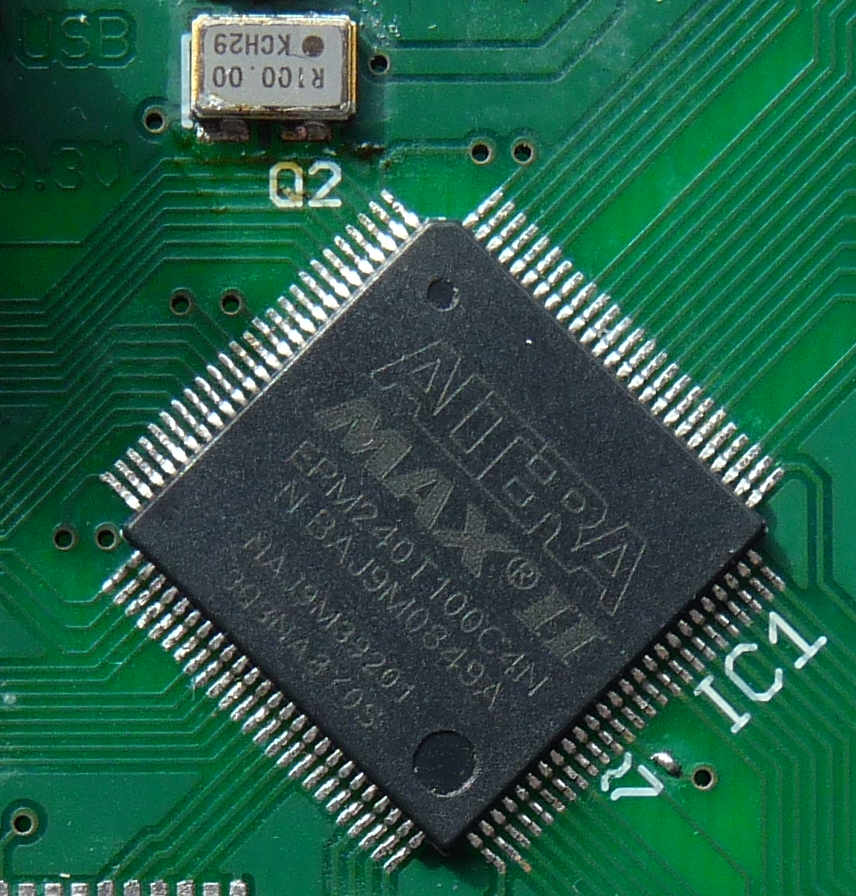
\includegraphics[width=0.3\textwidth]{images/CPLD_Photo.png}\\
	\rule{\linewidth}{0.5pt}
	\caption{CPLD mit Quarzoszillator (aufgel�tet auf Platine)}
\end{figure}

\section{Mikrocontroller} \index{Mikrocontroller} \index{USB} \index{Programmierschnittstelle} \index{Atmega32-U4}

Die Aufgabe des Mikrocontrollers ist es, eine Schnittstelle zwischen PC und Logibaustein zur Verf�gung zu stellen. Dazu z�hlen vor allem folgende Dienste:

\begin{itemize}
 \item Bereitstellen einer Verbindung zum PC (USB)
 \item Steuerung des Logikbausteines
 \item Auslesen des Messdatenspeichers
 \item Aufbereitung und �bertragung der Messdaten
 \item Zur Verf�gung stellen einer Programmierschnittstelle f�r den CPLD
 \item Eigene, einfach zu handhabende Programmierschnittstelle
\end{itemize}


In der Aufgabenstellung der Arbeit war gegeben, dass die Verbindung zwischen Mikrocontroller und PC nicht �ber einen zus�tzlichen Baustein erfolgen sollte. Solche Bausteine werden zum Beispiel von dem Chiphersteller FTDI produziert und stellen eine USB zu UART oder JTAG Verbindung zur Verf�gung.

Dadurch wurde die Auswahl auf Mikrocontroller mit integrierter USB-Schnittstelle beschr�nkt. Solche Mikrocontroller werden von mehreren Herstellern, mit unterschiedlichen Prozessorkernen und Speichergr��en hergestellt. Als Prozessorkern in der ben�tigten Leistungsklasse kamen 8051-Derivate oder die 8-Bit AVR-Kerne der Firma Atmel in die n�here Auswahl.

F�r den Logikanalysator wurde ein Mikrocontroller mit AVR-Kern verwendet. Dies liegt zum einen an der schon etwas veralteten Technologie der 8051-Derivate, zum anderen gibt es f�r die 8-bit AVR Familie sehr viele, kostenlos verf�gbare Compiler und Programmiertools. Atmel nennt diese Produktlinie AT90USB. Die einzelnen Mikrocontroller dieser Familie unterscheiden sich haupts�chlich in der Speichergr��e sowie den integrierten Schnittstellen, wie zum Beispiel Ethernet.

Der abschlie�end ausgew�hlte Mikrocontroller ist der Atmel Atmega32-U4. Dieser Mikrocontroller besitzt die f�r die Aufgabe minimal ben�tigten Schnittstellen und verf�gt �ber gen�gend Speicher. Zus�tzlich besitzt er noch weitere Schnittstellen, wie zum Beispiel ein 10-bit A/D-Wandler, um eine zuk�nftige Erweiterung des Analysators zu erm�glichen. Trotz der gro�z�gigen Ausstattung befindet sich der Mikrocontroller noch weit unter der Preismarke von 10,- � pro St�ck.

\begin{table}[h]
\begin{tabular}{|l|l|}
\hline
Eigenschaft 		& Gr��e / Wert 	\\
\hline \hline
Taktgeschwindigkeit	& 8 oder 16 MHz	\\
\hline
Arbeitsspeicher		& 2.5 KByte	\\
\hline
EEPROM-Speicher		& 1 Kbyte	\\
\hline
Flash-Speicher		& 32 KByte	\\
\hline
Schnittstellen (Auszug)	& USB 2.0	\\
			& SPI		\\
			& JTAG		\\
			& 10bit A/D-Wandler \\
\hline
Betriebsspannung	& 3.3 V	\\
\hline
\end{tabular}
\caption{Eigenschaften des Atmega32-U4}
\end{table}

Der verwendete Prozessortakt von 8MHz wird von einem Quarzoszillator erzeugt. Der f�r den Betrieb der USB-Schnittstelle notwendige 12MHz-Takt wird von einem internen Taktgenerator erzeugt. Porgrammiert werden kann der Mikrocontroller entweder �ber die integrierte JTAG-Schnittstelle oder, mit Hilfe eines Bootloaders, direkt �ber die USB-Schnittstelle. Die Programmierung des Atmega32-U4 ist in den Kapiteln \ref{Mikrocontroller_Software}, \ref{USB-Schnittstelle} und \ref{USB-JTAG} beschrieben. \cite{Atmel01}

\begin{figure}[h,c]
	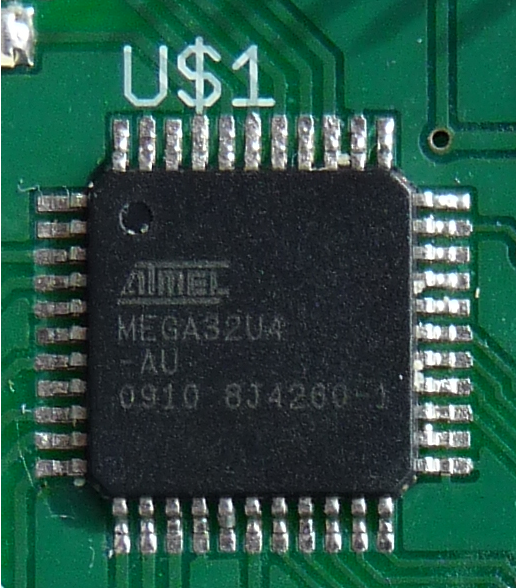
\includegraphics[width=0.3\textwidth]{images/Mikrocontroller_Photo.png}\\
	\rule{\linewidth}{0.5pt}
	\caption{Mikrocontroller (aufgel�tet auf Platine)}
\end{figure}

\section{Treiberbausteine} \index{Treiberbaustein} \index{Messf�hler}

Zwischen die IO-Pins des CPLD und den Messf�hlern wurden Treiberbausteine gesetzt. Der Grund daf�r ist vor allem der Schutz des CPLD vor Spannunsspitzen oder falscher Anwendung mit zu gro�en Spannungen. Im schlimmsten Fall sind dann zwar die Treiberbausteine defekt, jedoch liegen diese in einem wesentlich niedrigeren Preissegment als der CPLD und sind auch leichter austauschbar.

Ein weiterer Grund f�r die Verwendung der Treiberbausteine ist der Betrieb mit unterschiedlichen Spannungen. So wurden die Bausteine so gew�hlt, dass sie wahlweise mit Spannungen von 3.3V oder 5V an den Messf�hlern arbeiten. Diese Eingansspannung wird immer in die 3.3V IO-Spannung des CPLD gewandelt. Auch kann, f�r den Fall dass der Analysator als Logikgenerator betrieben wird, die 3.3V Ausgansspannung des CPLD in einen 5V Pegel gewandelt werden.

Anhand dieser Kriterien wurde nun der SN74LVC8T245 von Texas Instruments ausgew�hlt. Dieser Baustein verf�gt �ber insgesamt acht Treiber, so dass, f�r die 24 Messf�hler, drei dieser Bausteine ben�tigt werden. Zu beachten sind noch die unterschiedlichen Laufzeiten bei 3.3 V (0.8ns bis 6.3ns) und 5 V (0.8ns bis 4.4ns). Diese Laufzeitdifferenz muss in der Messfehlerberechnung mit einbezogen werden. \cite{Texas01}

\section{Speicherbausteine} \label{Speicherbausteine} \index{Speicherbausteine} \index{SRAM}

Die Auswahlkriterien des Speichers sind vor allem die ben�tigte Speichergr��e, sowie die m�glichst geringe Zugriffszeit, um eine schnelle Speicherung der Messergebnisse zu erm�glichen.

Als Speicherart kommt ein SRAM-Speicher \footnote{Static Random Access Memory} zum Einsatz. Dieser hat gegen�ber den DRAM-Speichern \footnote{Dynamic Random Access Memory} den Vorteil, dass die Ansteuerung des Speichers wesentlich einfacher gestaltet werden kann. Bei einem DRAM-Speicher m�sste der Speicherinhalt in regelm��igen Abst�nden aufgefrischt werden, da dieser sonst seine Informationen verliert. Durch die begrenzte Verf�gbarkeit an Logik im CPLD w�re eine solche Steuerung hier nicht realisierbar. Auch kann der SRAM-Speicher asynchron, also ohne Taktsteuerung, verwendet werden, was die Ansteuerung noch weiter vereinfacht.

Ein weiteres Kriterium ist die Datenbusbreite. Je breiter der Datenbus desto mehr Daten k�nnen auf einmal gespeichert werden. Dies verringert die Zeit, welche f�r das speichern und lesen einer bestimmte Menge an Daten ben�tigt wird. Jedoch erh�ht sich auch die Anzahl der ben�tigten IO-Pins am Logikbaustein. Am Logikbaustein ist eine der beiden IO-B�nke komplett f�r den Speicherzugriff vorgesehen. An dieser Bank befinden sich 40 IO-Pins zur freien Verf�gung. �bliche Datenbusbreiten sind 8, 16 und 32-Bit, wobei 32-Bit nicht praktikabel w�ren, da dann nur noch 8 Pins f�r die Adress und Steuerleitungen verf�gbar w�ren. Somit fiel die Wahl auf einen 16-Bit breiten Datenbus.

Die gesamte, maximale Speichergr��e ist nun abh�ngig von der Anzahl der restlichen, verf�gbaren IO-Pins. Dies wird in der nachfolgenden Tabelle verdeutlicht.

\begin{table}[h]

\begin{tabular}{|l|l|}
\hline
Steuerleitung 		& Anzahl \\
\hline \hline
Gesamt			& 40	\\
\hline
Datenbus		& 16	\\
\hline
Chip-Enable		& 1	\\
\hline
Read- und Write-Enable	& 2	\\
\hline
Byteauswahl		& 2	\\
\hline \hline
F�r Adressbus vef�gbar:	& 19	\\
\hline
\end{tabular}
\caption{Ben�gtigte Busleitungen}
\end{table}

Um eine flexiblere Best�ckung des Alysators zu erm�glichen, wurde entschieden den Speicher auf zwei Bausteine zu verteilen. Diese beiden Bausteine sind parallel �ber einen Speicherbus verbunden, wobei die Auswahl des aktiven Speichers durch ein seperates Chip-Enable Signal erfolgt. Durch dieses doppelte CE-Leitung verringert sich die maximale Breite des Adressbusses auf 18.

Somit besitzt jeder dieser beiden Speicher eine Gr��e von $2^{18} \cdot 16 Bit = 512 Kbyte$. Daher vef�gt der Analysator �ber ingesamt einen Megabyte an Speicher. Dadurch k�nnen, zum Beispiel bei einer Anwendung mit acht Messleitungen und 24-Bit Zeitstempel, bis zu 262.144 Messergebnisse gespeichert werden. Dies entspricht, bei einem durchschnittlichen Abstand von 1ms zwischen den Messwerten, einer Aufzeichnungszeit von �ber 260 Sekunden oder 4,3 Minuten.

Anhand dieser eingeschr�nkten Suchkriterien wurde der Speicherbaustein AS7C34098A von Alliance Memory ausgew�hlt. Er bestitzt genau die erw�hnte Buskonfiguration und verf�gt �ber eine geringe Zugriffszeit von 8ns. \cite{Allia01}



\section{Spannungsversorgung} \index{Spannungsregler} \index{LM1117}

Auch die Spannungsversorgung des Analysators sollte so variabel wie m�glich gestaltet werden. So kann die Versorgungsspannung sowohl nur �ber die USB-Schnittstelle, als auch durch ein externes Netzteil bereitgestellt werden. 

Der Schaltungsaufbau verf�gt �ber zwei unterschiedliche Spannungen. Eine 5V und eine 3.3V Spannungsdom�ne. Die 3.3V Versorgungsspannung wird von nahezu s�mtlichen Bausteinen verwendet. Lediglich die Treiberbausteine verwenden, f�r die Pegelwandlung, die 5V Betriebsspannung. 

Bei einer Spannungsversorgung �ber USB wird die 5V Spannungsdom�ne direkt von der USB-Spannung betrieben. Lediglich ein Gl�ttungskondesator ist zus�tzlich vorgesehn. F�r die Erzeugung der 3.3V sorgt ein LM1117-3.3 Spannungsregler von National Semiconductor. Dieser Regler erzeugt, aus einer beliebigen Spannung zwischen 4.25V und 10V, eine konstante Spannung von 3.3V, bei einem maximalen Strom von 800mA. Jedoch stellt die USB-Schnittstelle nur einen Strom von 500mA zur Verf�gung, so dass dieser bereits hier begrenzt ist. F�r die gesamte Schaltung wurde im Betrieb ein Stromverbrauch von unter 400mA gemessen, so dass hier keine Probleme zu erwarten sind.

Falls nur ein USB-Anschluss mit geringerem Maximalstrom zur Verf�gung steht, oder der Analysator unabh�ngig von USB betrieben werden soll, ist noch eine externe Spannungsversorgung vorgesehen. Diese kann mit 6.5V bis 12V betrieben werden. Ein LM1117-5.0 Baustein erzeugt daraus eine Spannung von 5.0V, welche dann, �ber einen Jumper ausw�hlbar, in den oben erw�hnten 5V-Kreis gespeist werden kann.
\chapter{Hardwareprototyp: Platinendesign} % Kapitel 3

\section{Einf�hrung} \index{Platinendesign}

Da die meisten verwendeten Baueile nur in SMD-Geh�usen produziert werden, ist es nahezu nicht m�glich die Schaltung auf einer Experimentier- oder Lochrasterplatine aufzubauen. Auch k�nnen nicht vorhersehbaren Seiteneffekte, die eine Experimentierplatine zum Beispiel auf die Laufzeiten an den Speicherbausteinen h�tte, auftreten. Aus diesem Grund war von Anfang an vorgesehen, den Prototyp der Schaltung auf einer ge�zten Platine aufzubauen. Aufgrund der Komplexit�t und Leiterbahndichte der Schaltung, ist dies nur durch CAD-Anwendungen \footnote{CAD: Computer Aided Design, dt: Rechnergest�tzter Entwurf} realisierbar. Sowohl f�r den Schalplanentwurf, als auch f�r das Platinenlayout wurde die CAD-Software ``EAGLE'' von Cadsoft verwendet, welche im folgenden Abschnitt genauer erl�utert wird.

\section{Designsoftware Cadsoft EAGLE} \index{EAGLE}

Die CAD-Software EAGLE ist ein relativ leicht anzuwendendes und schnell erlernbares Tool zur Erstellung von Schaltpl�nen und Platinenlayouts. Die Software ist bei einer nichtkomerziellen Anwendung komplett kostenlos, und daher bei Hobbyentwicklern und im Open-Hardware-Bereich sehr beliebt. Au�erdem ist die Software sowohl f�r Linux als auch f�r Windows verf�gbar. Die kostenlose Version hat jedoch die Enschr�nkung, dass nur zweiseitige Platinen, mit einer maximalen Gr��e von 100mm x 80mm erstellt werden k�nnen. Dies ist jedoch f�r dieses Projekt v�llig ausreichend. Die f�r das Projekt verwendete Softwareversion ist 5.7.0 f�r Linux.

F�r den Schaltplan und Platinenentwurf stehen eine gro�e Bauteilebibliothek zur Verf�gung. Falls man in dieser Bibliothek nicht f�ndig wird, so gibt es eine Vielzahl weiterer Biblitoheken im Internet, welche von einer gro�en Comunity gepflegt werden. F�r den Fall, dass das gesuchte Bauteil auch dort nicht auffindbar ist, kann man es im Bibliothekseditor selbst erstellen.

In der Oberfl�che selbst sind Schaltplan- und Platineneditor getrennt. Man kann mit den einzelnen Editoren seperat arbeiten, oder auch beide Editoren parallel verwenden. In diesem Fall wird zum Beispiel eine Bauteil�nderung im Schaltplan sofort auf der Platine Sichtbar. Vor allem in einer Multi-Monitor Umgebung ist diese Arbeitsweise zu empfehlen.

\section{Entwurf des Schaltplanes} \index{Schaltplan} 

Beim Entwurf des Schaltplanes sollte man zum gro�en Teil systematisch vorgehen. So wurde in dieser Arbeit zun�chst die gesamte Schaltung in mehrere Teilabschnitte unterteilt:

\begin{itemize}
 \item Spannungsversorgung
 \item Mikrocontroller
 \item Logikbaustein mit Speicher und IO
\end{itemize}

Die Spannungsversorgung enth�lt s�mtliche Bauteile, die aus den verschiedenen Eingansspannungen die n�tigen Versorgungsspannungen erstellen. Daf�r werden zwei LM1117 Bautsteine f�r 3.3V und 5V, mit den zugeh�rigen Gl�ttungskondensatoren, verwendet. Als Verpolungsschutz ist zus�tzlich eine Diode am Eingang angebracht. Die Spannungsquelle kann mittels eines Jumpers von Extern auf USB umgestellt werden. Die anliegende Versorgungsspannug wird �ber eine rote LED signalisiert. Siehe Abblildung \ref{pic:Spannungsversorgung}.

\begin{figure}[ht]
	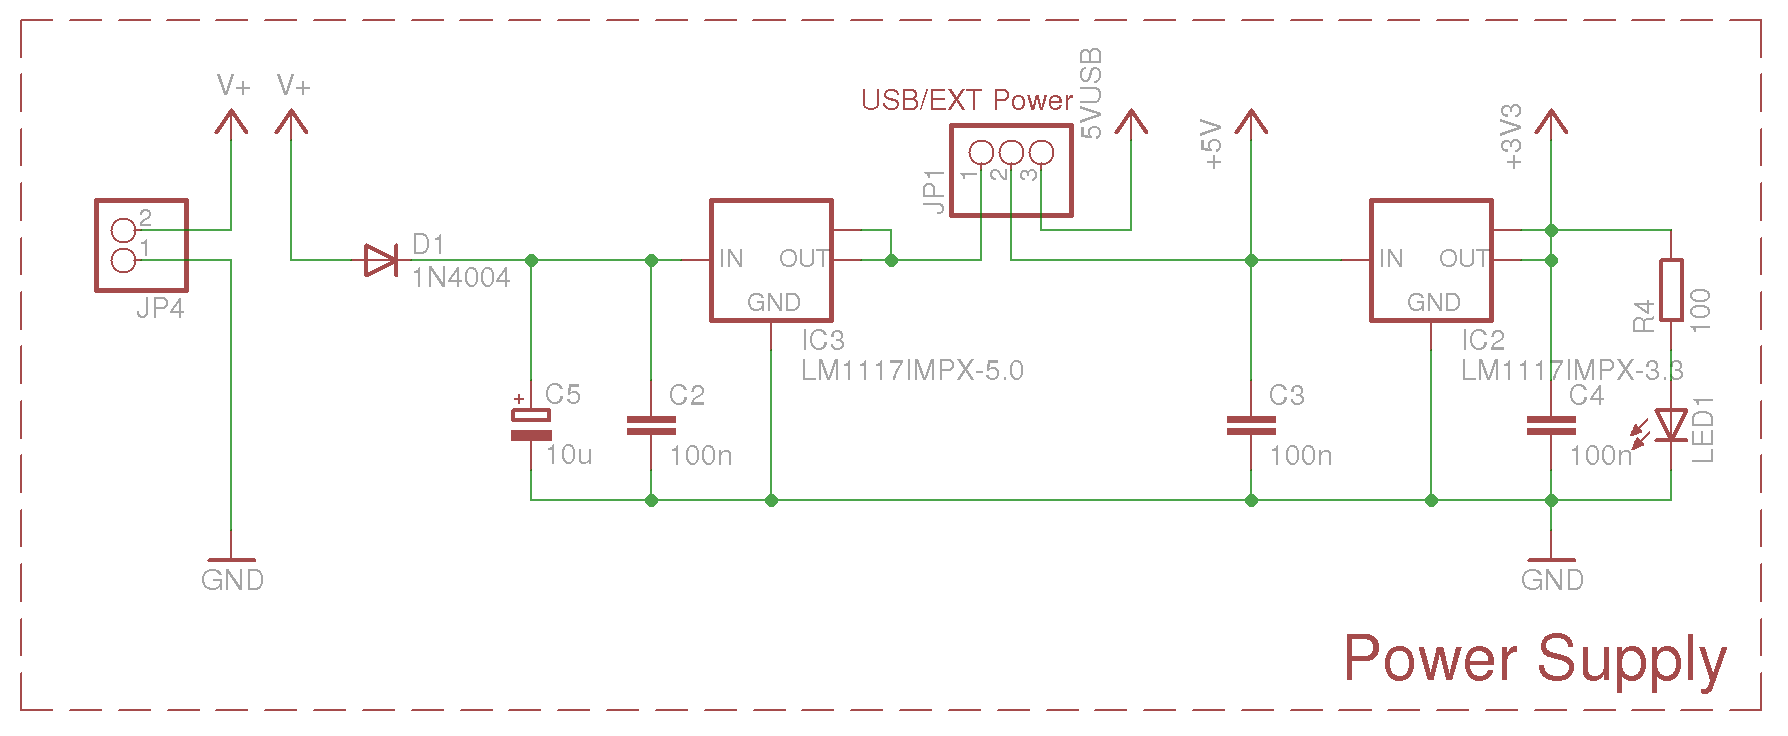
\includegraphics[width=1.0\textwidth]{images/Power_Supply.png}\\
	\rule{\linewidth}{0.5pt}
	\caption{Schaltplan der Spannungsversorgung}
	\label{pic:Spannungsversorgung}
\end{figure}


Der Abschnitt f�r den Mikrocontroller enth�lt s�mtliche Bauelemente die f�r die Grundfunktion des Prozessors n�tig sind. Dazu z�hlen vor allem die Beschaltung der Spannungsversorgung mit den diversen Abblockkondensatoren und der Anschluss des 8MHz Quarzozillators als Taktquelle. Ausserdem ist der USB-Stecker, zusammen mit den ben�tigten 22$\Omega$ Widerst�nden in der Datenleitung, eingeplant. 

F�r die Programmierung des Mikrocontrollers ist der 10-Polige Wannenstecker vorgesehen. �ber diesen wird eine JTAG-Verbindung realisert, wobei die Beschaltung des Steckers kompatibel ist zum Programmieradapter JTAG-ICE MKII von Atmel. F�r eine Signalisierung, von zum Beispiel einer Aktivit�t am USB-Anschluss, sind an zwei Ausg�ngen LEDs vorgesehen. 

Die LEDs werden als low-aktive Bauelemente beschaltet. Das bedeuted, dass der Ausgang des Mikrocontrollers auf logisch 0 (Masse) gesetzt wird, um die LED einzuschalten. Dadurch wird der Betriebsstrom f�r die LED nicht durch den Mikrocontroller, sondern durch die am Vorwiderstand abfallende Betriebsspannung erzeugt. Dies hat den Grund, dass der Stromflu� von au�en durch den Mikrocontroller wesentlich h�her sein kann, als der Strom welcher an den Ausgangspins zur Verf�gung stehen w�rde.

Der Reset-Eingang des Atmega ist mit einem Reset-Strang verbunden. Da der Reset Eingang lowaktiv ist, wird der Reset-Strang �ber einen 4.7k$\Omega$ Widerstand auf die Betriebsspannung gezogen. �ber einen Jumper (JP6) kann die Leitung auf Masse gesetzt, und damit der Reset ausgel�st werden. Ausserdem ist die Resetleitung noch mit dem Programmieranschluss verbunden, so dass der Programmieradapter auch einen Reset ausl�sen kann. Als weiteres Bauteil kann der CPLD �ber eine L�tbr�cke mit dem Reset verbunden werden.

\begin{figure}[ht]
	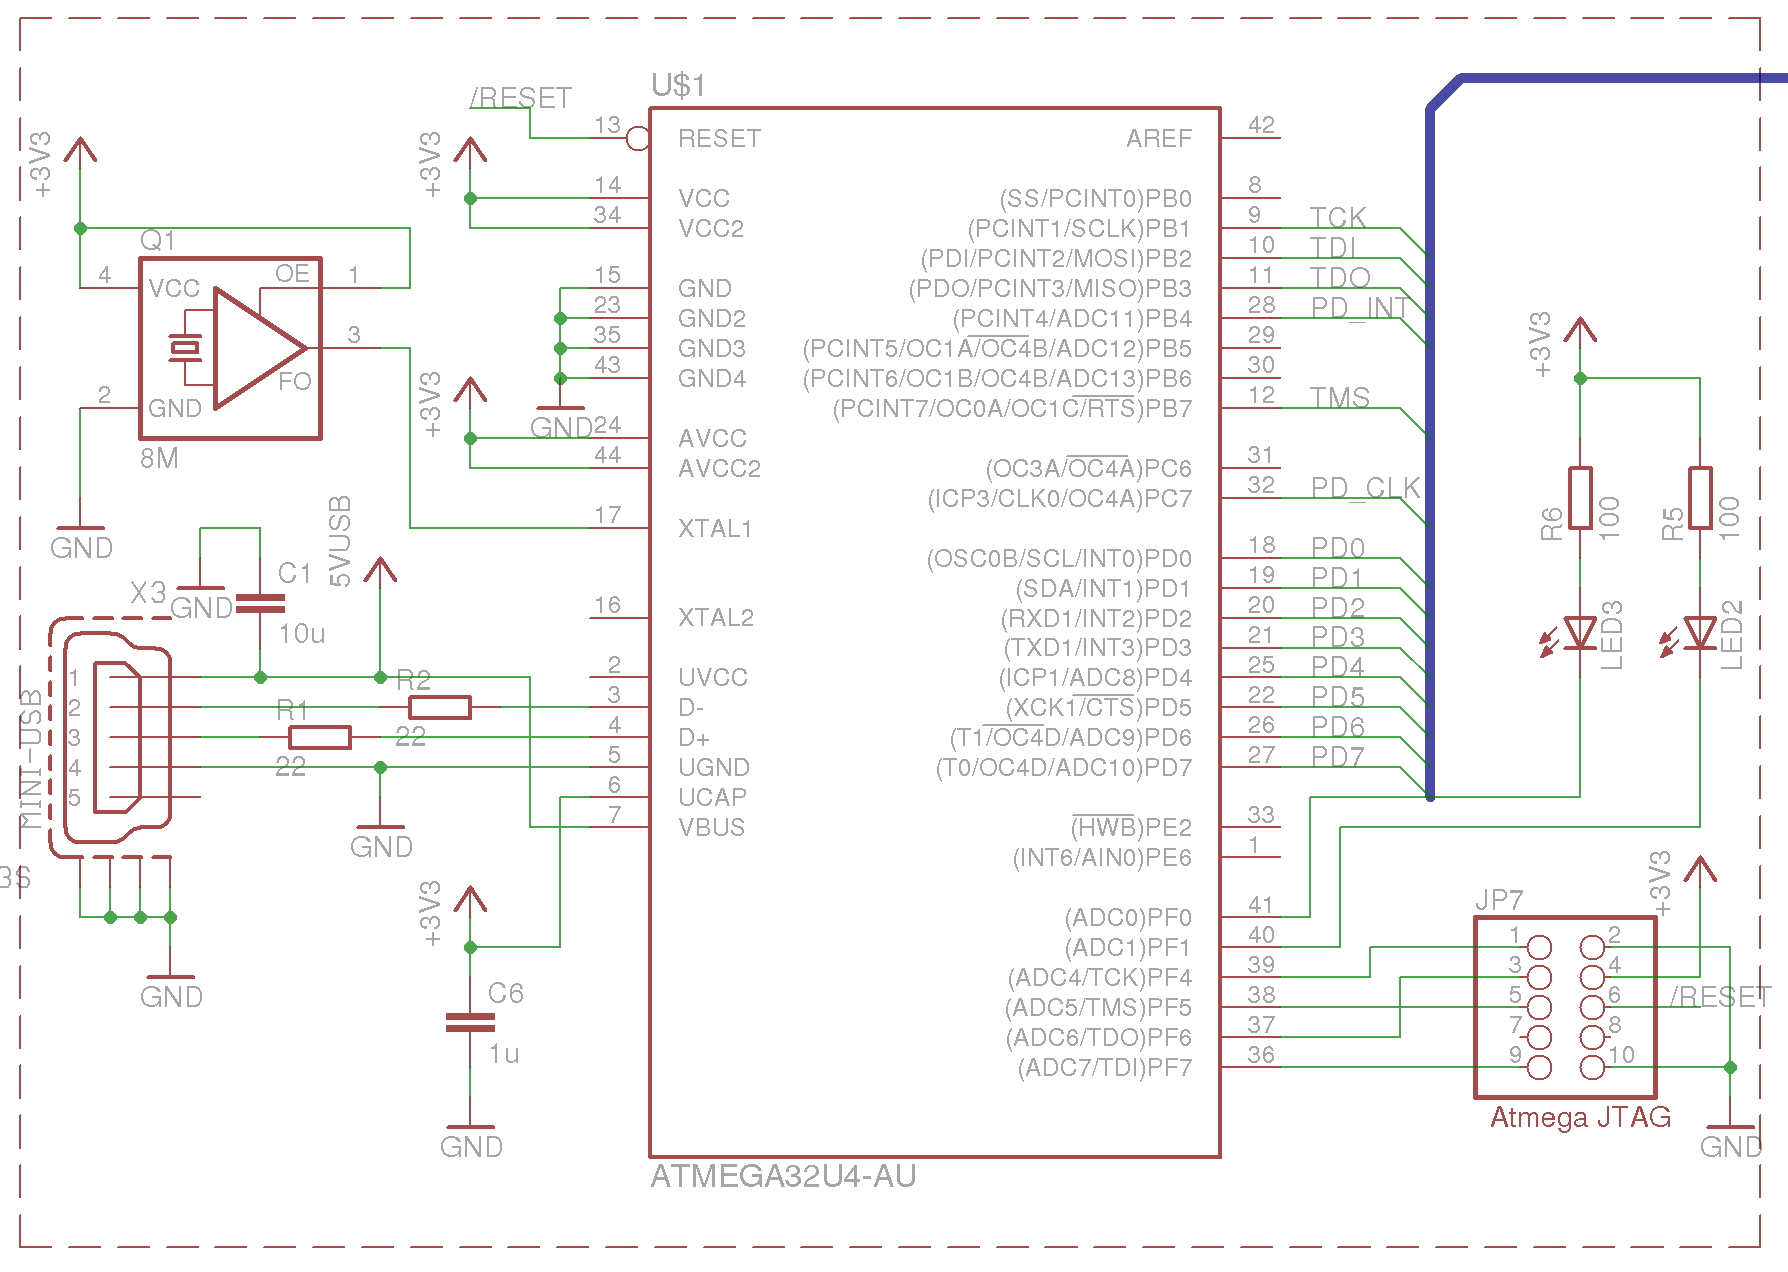
\includegraphics[width=0.66\textwidth]{images/Mikrocontroller.png}\\
	\rule{\linewidth}{0.5pt}
	\caption{Grundschaltung des Mikrocontrollers}
	\label{pic:Mikrocontroller}
\end{figure}

Die Grundbeschaltung des CPLD ist auch relativ einfach. Zur Stabilisierung der Spannungsversorgung sind f�r die beiden IO-B�nke je ein, und f�r die Kernversorgung zwei Abblockkondensatoren vorgesehen. An einen der vier verf�gbaren Takteing�nge ist ein 100 MHz Quarzoszillator angeschlossen. Ein weiterer Takteingang kann �ber eine L�tbr�cke mit dem oben beschriebenen Reset-Strang verbunden werden. Dadurch kann ein externer, asynchroner Reset ausgel�st werden. Jedoch ist darauf zu achten, dass ein unkonfigurierter CPLD, auf Grund der undefinierten Pinzust�nde, den gesamten Reset-Strang aktiv schalten kann. Dadurch kann der Mikrocontroller in einen gesprerrten Zustand versetzt werden. Daher ist darauf zu achten, die L�tbr�cke nur dann zu setzen, wenn der entsprechende Pin als hochohmiger Eingangspin beschaltet ist.

Die Verbindung zu den Speichern erfolgt direkt �ber einen parallelen Bus ohne zus�tzliche Beschaltung. Mit dem Mikrocontroller ist der CPLD �ber einen 8-bit breiten Bidirektionalen Bus, mit seperater Interrupt und Taktleitung, verbunden. Somit k�nnen verschiedene synchrone oder asynchrone Bussysteme implementiert werden. Als Programmierschnittstelle ist eine JTAG Schnittstelle vorgesehn. Sie ist �ber eine vierpolige Stiftleiste verwendbar. Diese Stiftleiste kann auch mit vier Jumpern zum Mikrocontroller gebr�ckt werden, so dass dieser als USB-Programmieradapter verwendet werden kann. Siehe Kapitel \ref{USB-JTAG}.

Die Speicherbausteine sind nur mit dem CPLD und der Spannungsversorgung verbunden, da laut Datenblatt keine spezifische Beschaltung notwendig ist. Die Bustreiber sind auf der B-Seite mit 24-IO-Pins des CPLD verbunden. Die A-Seite f�hrt zu einem 28-poligen Wannenstecker, wobei an jeweils zwei der Pins eine Versorgungsspannug sowie der Masseanschluss anliegt. Die Auswahl der Messpannung an der A-Seite erfolgt �ber einen Jumper und kann zwischen 3.3V und 5V ausgew�hlt werden. Die Steuerleitung f�r die Signalrichtung (A nach B oder umgekehrt) ist ebenfalls direkt mit dem CPLD verbunden. Siehe Schaltplan im Anhang.

\section{Entwurf des Platinenlayoutes} \index{Platine} \index{Leiterbahn} \index{Luftlinien} \index{Massefl�che}

Das Entwerfen der Platine unterteilt sich nun in mehrere Abschnitte. Zun�chst versucht man die Bauteile im Platineneditor m�glichst in den logische Gruppen anzuordnen. Also zum Beispiel alle Bauteile f�r die Spannungsversorgung m�glichst nahe beieinander zu plazieren. Den CPLD als zentraler Baustein mit Verbindungen zu allen Seiten sollte auch m�glichst zentral plaziert werden.

F�r die weitere Ausrichtung und Plazierung aller Bauelemente, stellt EAGLE sogenannte Luftlinien zur Verf�gung. Das sind logische Verbindungen, die den Leiterbahnen im Schaltplan entsprechen und die einzelnen, zusammenh�ngenden Pins optisch miteinander verbinden. Nun ordnet man die Bauteile m�glichst so an, dass sich die Luftlinien m�glichst wenig kreuzen, denn so ist ein Layout mit m�glichst wenig Durchkontaktierungen m�glich. Auf die Benutzung des Autorouters, welcher die Leiterbahnen vollautomatisch erstellt, sollte m�glichst verzichtet werden, da dessen Routinen nicht ausgereift sind, und so mehr ein Wirrwar entsteht als eine Leiterplatte.

Nun geht man Luftlinie f�r Luftlinie vor. Zun�chst w�hlt man die gew�nsche Breite der Leiterbahn. Als n�chstes werden m�glichst kreuzungsfrei die Pins der Bauelemente zu verbunden. Ist dies nicht m�glich, wechselt kann man auf den anderen Layer der Platine. Dabei werden automatisch die entsprechenden Durchkontaktierungen erzeugt.

Begonnen wurde bei dieser Arbeit mit der Spannungsversorgung in der linken oberen Ecke. Es wurde jedoch auf das Routen der Leiterbahn f�r die Masse verzichtet, da die Masse sp�ter durch eine komplette Massefl�che ersetzt wird. Die Leiterbahnen f�r die Spannungsversorgung wurden m�glichst breit gestaltet. Dies hat zum einen den Grund den Widerstand aufgrunde der h�heren Str�me zu minimieren, zum anderen werden bei den LM1117-Bausteinen die Anschlusspins f�r die geregelte Spannung, gleichzeitig als K�hlfl�chen benutzt. Deshalb wird durch die breiteren Leiterbahnen f�r eine bestm�gliche W�rmeabfuhr gesorgt.

\begin{figure}[ht]
	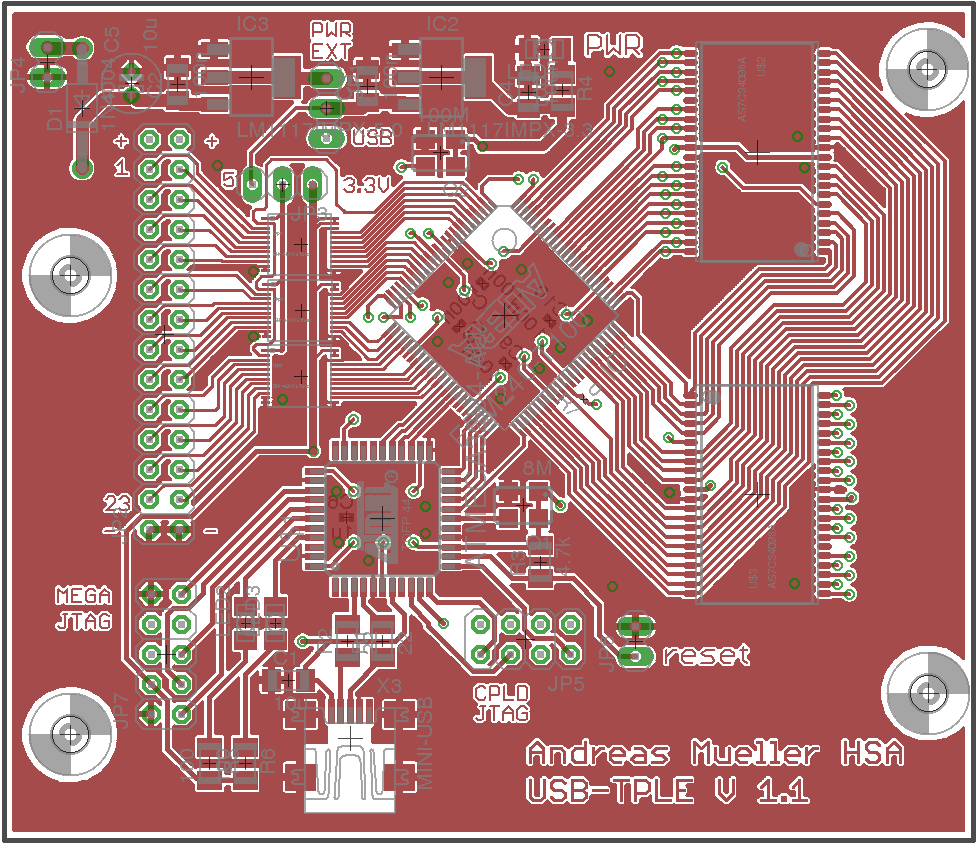
\includegraphics[width=0.6\textwidth]{images/Platine_top.png}\\
	\rule{\linewidth}{0.5pt}
	\caption{Oberseite der Platine}
	\label{pic:Platine_top}
\end{figure}

Als n�chstes wurde der Atmega m�glichst nahe am USB-Anschluss plaziert. Alle weiteren Bauteile, wie die LEDs und der Programmieranschluss, wurden in unmittelbarer Umgebung positioniert, um m�glichst kurze Leiterbahnen zu erm�glichen. Die Spannungsversorgung des Atmega wurde durch eine U-f�rmige Leiterschleife innerhalb der Anschlusspins verwirklicht. Dadurch k�nnen die �brigen Pins, ohne Durchkontaktierungen, problemlos nach au�en verbunden werden. Siehe Abbildung \ref{pic:Platine_top} und \ref{pic:Platine_bot}, Bauteil U\$1.

Das komplexeste Layout ist der Speicherbus. Dieser verbindet den CPLD mit den beiden Speichern �ber einen parallelen Bus mit 40 Leitungen. Diese 40 Leitungen sind in der Form einer 8 an die Pins der Speicherbausteine angeschlossen und mit dem CPLD verbunden. Um dies bei m�glichst gleichbleibender Leitungsl�nge zu erm�glichen, ist der CPLD in einem um 45� versetzen Winkel plaziert. Die Spannungsversorgung des CPLD wurde �hnlich der des Mikrocontrollers verwirklicht. 

Als letzte Bauteile wurden die Bustreiber, zusammen mit dem Anschlusstecker f�r die Messleitungen, plaziert und verbunden. Nun kann das, in EAGLE integrierte, Testprogramm aufgerufen werden. Dieses Testprogramm weist auf m�gliche Routingfehler, wie zum Beispiel Kurzschl�sse oder zu kleine Abst�nde, hin.

Zum Schluss wird f�r die Masseanbindung aller Bauteile, eine Massefl�che �ber die gesamte Oberseite, und zeilweise �ber die Unterseite, verwirklicht. Eine Massefl�che verhindert das Entstehen von Masseschleifen. Bei einer Masseschleife geht die Leiterbahn, welche das Massepotential tr�gt, rings um die gesamte Leiterplate, um zu allen Bauelementen zu gelangen. Diese Leiterbahn kann wie eine Antenne f�r einfallende St�rsignale wirken und so die Funktion der Schaltung stark beeintr�chtigen. Durch die gleichm��ige Verteilung der Massefl�che wird dies verhindert und zus�tzlich werden die restlichen Leiterbahnen von der umliegenden Masse gegen St�rungen geschirmt. Die beiden Massefl�che der Ober- und Unterseite, sollten durch mehrere Durchkontaktierungen verbunden werden, um einem m�glichen Kondensatoreffekt entgegenzuwirken. 

Nach Abschluss k�nnen die Platinendaten in ein f�r die Herstellung passendes Format, wie zum Beispiel PDF, exportiert werden. Meist ist es m�glich, die EAGLE Dateien auch direkt zu einem professionellen Platinenhersteller zu schicken.


\begin{figure}[ht]
	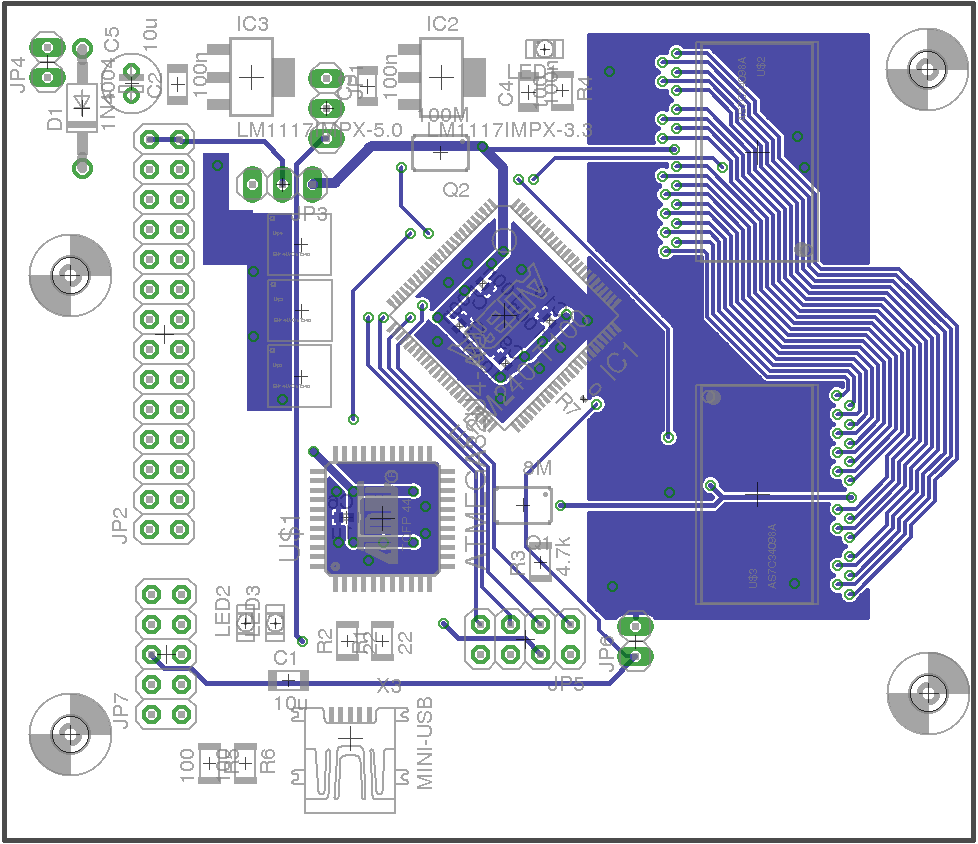
\includegraphics[width=0.6\textwidth]{images/Platine_bot.png}\\
	\rule{\linewidth}{0.5pt}
	\caption{Unterseite der Platine}
	\label{pic:Platine_bot}
\end{figure}

\section{Aufbau und Test des Prototypen} \index{Prototyp} \index{L�ttechnik}

Die Platine wurde von einem professionellen Platinenhersteller (Multi PCB \footnote{Multi PCB: http://www.multipcb.de/}) ge�zt. Durch die professionelle Herstellung sind auch bereits alle Durchkontaktierungen vorhanden und die Platine wurde elektrisch gepr�ft. Die Platine ist mit L�tstopplack sowie einer Beschriftung versehen, was den Aufbau des Analysators erheblich erleichtert.

Beim Best�cken der Platine geht man nun �hnlich systematisch vor, wie beim Routen der Leiterbahnen. Man unterteilt die Platine in mehrere funktionelle Teilabschnitte. Diese werden nacheinander aufgebaut, und es wird erst mit dem n�chsten Abschnitt begonnen, wenn der vorherige zumindest kurz auf Funktion �berpr�ft wurde.

Begonnen wurde mit der Stromversorgung, da ohne diese auch alle weiteren Abschnitte nicht funktionieren w�rden. Dazu wurden zun�chst alle SMD-Bauteile aufgel�tet. Die daf�r verwendet Temperatur des L�tkolbens ist abh�ngig vom verwendeten Lot, liegt jedoch bei ungef�hr 300�C. Um dies ohne professionellel SMD-Werkzeug zu erm�glichen, bedient man sich eines kleinen Tricks: Zun�chst bringt man etwas L�tzinn auf die Spitze des L�tkolbens auf. Nun plaziert man mit einer Pinzette das Bauteil (z.b. Widerstand) an der richtigen Stelle und fixiert es an einer Seite kurz mit dem L�tkolben. Nun hat man die andere Hand wieder frei um die zweite Seite sauber anzul�ten. Zum Schluss ersetzt man die kurze Fixierung vom Anfang durch eine Saubere L�tstelle. Als letztes werden nun die drahtgebundenen Bauteile, wie die Anschlusspins, aufgel�tet.

Nun kann die Funktion des Spannungsreglers �berpr�ft werden. Nach einer Sichtpr�fung auf eventuelle Kurzschl�sse oder L�tbr�cken kann die Versorgungsspannung angelegt werden. Um hier evetuellen Schaden durch Kurzschl�sse zu vermeiden, sollte ein geregeltes Labornetzeil, mit niedrig eingestelltem Strombegrenzer, verwendet werden. Nun wird zun�chst die 5V Spannungsdom�ne mit einem Multimeter durchgemessen. Ist hier eine stabile Spannung, bei einem sehr geringen Stromverbrauch von wenigen mA, vorhanden, kann der Jumper f�r die Versorgung des 3.3V Spannungsreglers gesetzt werden. Ist auch an diesem eine konstante Spannung von 3.3V zu messen, sollte auch die Betriebs-LED leuchten. Als n�chstes kann mit dem Aufbau des n�chsten Abschnitts begonnen werden.

Der n�chste Abschnitt ist der Aufbau des Mikrocontrollers. F�r dessen Aufl�ten muss man sich, aufgrund der geringen Pinabst�nde, folgenderma�en behelfen. Man fixiert zun�chst den Chip an zwei gegen�berliegenden Ecken mit der selben Methode wie bei den SMD-Widerst�nden. Nun kann man Seite f�r Seite vorgehen, ohne den IC weiter fixieren zu m�ssen. Nun versucht man m�glichst jedes Beinchen kurz zu erhitzen und mit gen�gend L�tzinn zu befestigen. Als Hilfe dient hier etwas Flussmittel. Dabei werden bei einer Standard-L�tspitze mit sicherheit einige Br�cken zwischen den Pins entstehen. Das ist aber nicht weiter problematisch. Nachdem eine Seite fertig gel�tet wurde, benutzt man eine Entl�tlitze um die entstandenen L�tbr�cken wieder zu entfernen. Dazu legt man die Litze quer �ber alle 11 Pins und erhitzt diese mit dem L�tkolben. Beim Anl�ten des Oszillators liegt die Schwierigkeit darin, dass sich die L�tfl�chen auf desssen Unterseite befinden. Jedoch mit etwas mehr Flussmittel wird beim Erhitzten das Lot unter den Baustein ``gesogen''.

Nachdem nun der Abschnitt f�r den Mikrocontroller fertig aufgel�tet ist, sollte auch dieser zun�chst optisch auf Kurzschl�sse �berpr�ft werden. Nun kann die Versorgunsspannung mit eingestelltem Strombegrenzer (ca. 100mA) angelegt werden. Zur �berpr�fung der Funktion kann mit dem JTAG-ICE-MKII Programmierkabel ein kleines Testprogramm aufgespielt werden. Dieses Testprogramm kann z.B. alle Ausgangspins im Sekundentakt Ein- und Ausschalten, welche dann durchgemessen werden.

Als n�chsten Arbeitsschritt wird nun der CPLD aufgel�tet. Daf�r wird, aufgrund der �hnlichen Geh�useform, genauso vorgegangen wie beim Mikrocontroller. Zwar ist der Pinabstand hier noch geringer, jedoch noch gut von Hand l�tbar. Getestet wird der CPLD �ber die JTAG-Schnittstelle. Dazu werden die vier Jumper an JP5 entfernt. Als Programmierger�t ist ein Altera-USB-Blaster am besten geeignet. Mit einer sogenannten Peitsche, also einem 10-poligen Programmierkabel mit einzelnen flexiblen Leitern, wird nun der Byteblaster mit der Platine verbunden. Dazu m�ssen jediglich die vier JTAG-Leitungen (TDI, TDO, TCK und TMS), sowie die Spannungsversorgung (+3.3V und GND) angeschlossen werden. Weitere Verbindungen, wie Reset, sind nicht notwendig. Nun kann ein kleines Testprogramm zum Auslesen der ID-Codes verwendet werden. Es ist auch m�glich, ein kleines Projekt mittels der Altera Software ``Quartus II'' zu erstellen und aufzuspielen.

Jetz k�nnen die Speicherbausteine und die Bustreiber auf die gleiche Weise aufgel�tet werden. Die Bustreiber lassen sich in Ausgangsrichtung durch einen im CPLD implementierten Schieberegister testen. In Eingangsrichtung k�nnte man die Signale in den Speicherbausteinen zwischenspeichern und zur�ckschicken. Dadurch w�ren auch die Speicherbausteine getestet. Dieser Test wurde jedoch im Rahmen dieser Arbeit noch nicht vollst�ndig durchgef�hrt.

\begin{figure}[ht]
	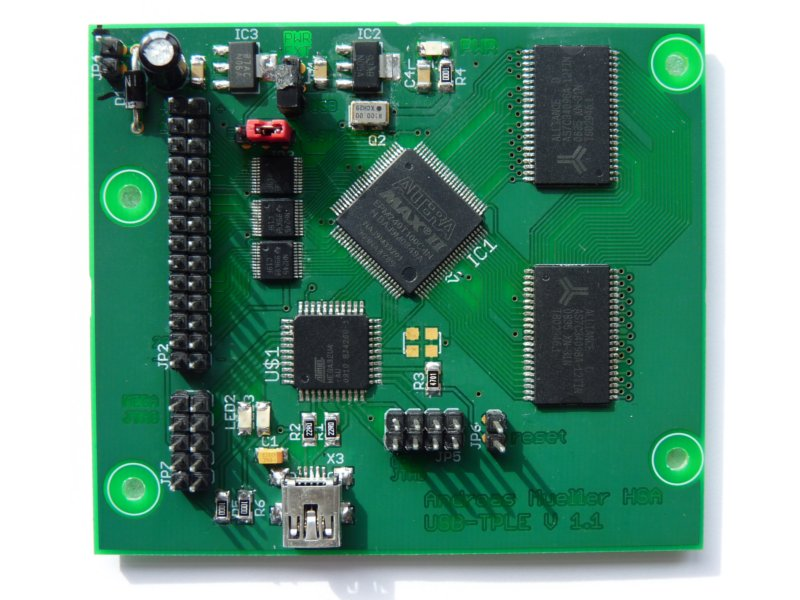
\includegraphics[width=0.7\textwidth]{images/board.jpg}\\
	\rule{\linewidth}{0.5pt}
	\caption{Fertig aufgebauter Prototyp}
	\label{pic:Prototyp}
\end{figure}


\section{Bekannte Fehler im Prototyp} \index{Prototyp}

Der einzige bekannte Fehler im Prototyp der Version 1.1, ist ein Fehler in der Beschaltung der Bustreiber. Das Problem liegt hierbei in der Tatsache, dass der Spannungspegel f�r die Steuerleitung $\overline{DIR}$ von dem Spannungspegel der A-Seite bestimmt wird. Wird die Messpannung nun auf 5V gestellt, so reichen die 3.3V Spannung des CPLD nicht aus, um diese Leitung zu schalten. Somit ist ein sicherer Betrieb nur im 3.3V-Modus m�glich. In einem zuk�nfitigen Prototyp kann einfach die A-Seite und B-Seite des Bustreibers getauscht werden, so dass die A-Seite immer mit 3.3V und die B-Seite Variabel beschaltet wird.




\chapter{Mikrocontroller Software} \label{Mikrocontroller_Software}

\section{Einf�hrung}

In diesem Kapitel wird beschrieben, wie die Programmierung f�r den Mikrocontroller erfolgt. Als Programmiersprache kommt C zum Einsatz. Die Firmware des Mikrocontrollers muss so konzipert werden, dass sie alle Aufgaben, die zur Funktion des Analysators notwendig sind, ausf�hren kann. Dazu z�hlen vor allem die Schnittstellenfunktion zwischen PC und CPLD, und die F�higkeit die Firmware beider Bausteine (Mikrokontroller und CPLD) �ber USB aktualisieren zu k�nnen. Eine genaue Beschreibung der USB-Schnittstelle und des USB-JTAG-Adapters befindet sich in den Kapiteln \ref{USB-Schnittstelle} und \ref{USB-JTAG}.

\section{Entwicklungsumgebung} \index{Entwicklungsumgebung} \index{Linux} \index{Windows}

Als Entwicklungsrechner wurde ein Standard x86-PC mit den folgenden Spezifikationen verwendet:\\

% use packages: array
\begin{tabular}{ll}
Prozessor: & Pentium IV, 2.8 GHz, HT \\ 
Arbeitsspeicher: & 1 GB DDR2 \\ 
Chipsatz: & Intel 865 \\ 
Betriebssystem: & Windows 7
\end{tabular}\\

Die Entwicklungsumgebung zur Erstellung der Firmware des Mikrocontrollers besteht, auf Softwareseite, aus dem kostenlos erh�ltlichen AVR-Studio in der Version 8 von Atmel. Das AVR-Studio enth�lt neben dem Quelltexteditor und einer Projektverwaltung auch eine integrierte Toolchain. Mit dieser Toolchain lassen sich die entwickelten Programme direkt kompilieren und �ber einen Programmieradapter auf den Mikrocontroller spielen. Zus�tzlich ist in dem AVR-Studio noch ein leistungsf�higer Debugger integriert. Mit dem Debugger lassen sich, unter der Vorraussetzung, dass der Programmieradapter und der Prozessor dies unterst�tzen, die Programme zur Laufzeit analysieren.

Es ist jedoch auch problemlos m�glich jede andere Toolchain, welche die f�r den Mikrocontroller passenden Entwicklungswerkzeuge enth�lt, zu verwenden. Dazu z�hlen ein f�r AVR-Prozessoren geeigneter Compiler (z.B. avr-gcc), ein Linker (z.B: avr-ld), eine passende Standard C-Bibliothek, sowie eine Software zum Aufspielen der Firmware (z.B. avrdude). Diese Tools sind f�r die meisten g�ngigen Betriebssysteme vorkompiliert, oder als Quellcode vef�gbar.

Als Programmieradapter wurde der JTAG-ICE-MKII von Atmel verwendet. Mit diesem Adapter l�sst sich der JTAG-Anschluss des Mikrocontrollers direkt �ber USB mit dem PC verbinden. Der JTAG-ICE-MKII wird vollst�ndig vom AVR-Studio unterst�tzt, was auch die Verwendung des integrierten Debuggers erm�glicht.

Um einige plattform�bergreifende Aspekte zu testen, wurde auf dem Entwicklungs-PC eine virtuelle Maschine mit einem Linux Betriebssystem installiert. Dazu wurde die kostenlose VMware-Player Version von VMware Inc. \footnote{http://www.vmware.com/de/} verwendet. Als Gastbetriebssystem kam die Linuxdistribution Debain in der Version 5.0 (Lenny) zum Einsatz.

\section{USB-Bootloader} \index{Bootloader}

Ein Bootloader ist ein eigenst�ndiges Programm, welches es erm�glicht, den Speicher eines Bausteins ohne externes Programmierger�t zu beschreiben. Der Bootloader �bernimmt dabei die Aufgaben den Flash des Bausteins zu l�schen, den zum Beispiel �ber USB gesendeten Datenstrom in ein entsprechendes Format zu wandeln um den Flash-Speicher anschie�end zu beschreiben. Im Falle des verwendeten Atmega32-U4, ist der f�r den Bootloader vorgesehene Specherbereich am oberen Ende des Flash-Speichers vorgesehen. Dies hat zur Folge, dass es dem Bootloader nur m�glich ist den Speicherbereich unterhalb dieser Adresse zu beschreiben, da er sich nicht selbst updaten kann. Der Bootloader selbst kann also nur durch einen externen Programmieradapter, wie den JTAG-ICE-MKII, aufgespielt werden.

Da sich nun zwei eigenst�ndige Programme im Speicher des Mikrokontrollers befinden, der Bootloader sowie die eigenliche Anwendung, gibt es nun verschiedene Mechanismen f�r die Auswahl, welches gestartet werden soll.

Beim Atmega gibt es nun drei verschiedene Konzepte: Eines dieser Konzepte sieht vor, dass der Prozessor immer von der Speicheradresse des Bootloaders (0x3800) startet. Dazu muss die BOOTRST-Fuse des Mikrocontrollers gesetzt werden. So kann man nun entweder ein neues Programm aufspielen, oder den Bootloader dazu veranlassen die Programmausf�hrung an der Startadresse 0x0 fortzusetzen. Dies kann zum einen �ber einen per USB gesendeten Befehl, oder �ber einen Timer erfolgen.

Ein anderes Konzept sieht vor, dass der Prozessor immer bei der Startadresse 0x0 mit der Programmausf�hrung beginnt. Wird nun an einem bestimmten Externen Pin () eine logische 0 angelegt, und danach der Hardware-Reset bet�tigt, so springt der Prozessor nach dem Reset an die Startadresse des Bootloaders.

Eine dritte M�glichkeit ist es den Bootloader direkt aus dem Anwendungsprogramm herraus zu starten. Dazu wird der Watchdog verwendet. Der Watchdog hat normalerweise die Aufgabe, eine St�rung um Programmablauf zu identifizieren um bei einem Fehler einen Reset auszul�sen. Man kann jedoch nun in der Anwendungssoftware den Startvektor des Watchdogs auf die Startadresse des Bootloaders setzen, und den Watchdog im Anschluss ausl�sen lassen. Dadurch wird ein Reset mit der anschlie�enden Startadresse 0x3800 ausgel�st.

\subsection{Atmel-Bootloader} 

Der Atmel Bootloader f�r den Atmega32-U4 kann als vorkompilerte HEX-Datei von der Homepage bezogen werden. Der Quellcode kann auf Anfrage per Email direkt von Atmel bezogen werden. Standardm��ig ist der Bootloader bereits auf fabrikneuen Bausteinen aufgespielt, so dass der Programmiervorgang ohne Programmieradapter sofort m�glich ist. Jedoch ist darauf zu achten, dass beim nachtr�glichen programmieren �ber einen externen Programmieradapter meist der gesamte Flash, also auch der Bootsektor, gel�scht wird. Somit muss der Bootloader im Anschluss neu aufgespielt werden.

Wird der Mikrocontroller �ber den integrierten USB-Controller nun an den PC angeschlossen, so meldet sich der Controller als eine DFU-Klasse \footnote{DFU: Device Firmware Upgrade} am Host des PCs an. Die entsprechenden Parameter sind 0x03EB f�r die VID \footnote{VID: Vendor ID} von Atmel und 0x2FF4 f�r die PID \footnote{PID: Product ID} des Atmega32-U4 Bootloaders.

Nun k�nnen �ber den USB-Anschluss verschiedene Befehle, wie zum Beispiel f�r das Auslesen des Status, gesendet werden. Die genauen Befehle sind in dem Datenblatt des USB-DFU-Bootloaders enthalten \footnote{USB DFU Bootloader Datasheet: http://www.atmel.com/dyn/resources/prod\_documents/doc7618.pdf}. Man kann jedoch auch eine einfache Programmiersoftware wie den FLIP-Programmer von Atmel verwenden. Auf diesen Punkt wird weiter unten genauer eingegangen.

\subsection{LUFA-Bootloader}

LUFA \footnote{LUFA: Lightweight USB Framework for AVRs} ist ein von dem Australier Dean Camera entwickelter USB-Stack f�r alle Mikrocontroller der Atmel AT90-Serie, wozu auch der verwendete Atmega32-U4 geh�rt. Auf alle M�glichkeiten die dieses USB-Framework bietet, wird im Kapitel \ref{USB-Schnittstelle} noch genauer eingegangen. Das gesamte Projekt steht unter der MIT-Lizenz \footnote{MIT: Massachusetts Institute of Technology} wodurch eine uneingeschr�nkte Nutzung des Quellcodes m�glich ist.

Zu dem LUFA-Projekt z�hlt unter anderem auch ein DFU-kompatibler Bootloader. Dieser Bootloader kann die gleichen Befehle wie der original Atmel Bootloader verarbeiten. Er kann problemlos f�r den Atmega32-U4 kompiliert werden. Es muss dazu einfach im Makefile der Mikrocontrollertyp und die Startadresse des Bootsektors angegeben werden.

\begin{lstlisting}[caption=Einstellungen im DFU-Makefile]
MCU = Atmega32U4
BOOT_START = 0x3800
\end{lstlisting}

Um die Windowstreiber f�r den DFU-Bootloader von Atmel nutzen zu k�nnen, sind in der Datei ``Descripors.h'' bereits die oben erw�hnten PID und VID von Atmel eingetragen. Durch die Auswahl der entsprechenden MCU im Makefile werden diese ausgew�hlt.

Dadurch verh�lt sich der LUFA DFU-Bootloader genauso wie das Original von Atmel, und kann auch mit den selben Tools verwendet wrden. Er steht jedoch unter einer Open-Source Lizenz und kann problemlos an die eigene Anwendung angepasst werden. \cite{Lufa01}

\subsection{PC-Software} \index{FLIP} \index{DFU-Programmer}

Um den DFU nutzen zu k�nnen, ist auf der PC-Seite eine Software n�tig welche die Steuerung des Bootloaders �bernimmt. Dazu z�hlen neben dem Auslesen des Bootloader Status vor allem das L�schen, Beschreiben und Auslesen des Flash-Speichers. Zum Beschreiben muss nach der L�schung die vom Compler erzeuge HEX-Datei ausgelesen, und �ber den USB-Anschluss an den Bootloader �bertragen werden. 

Mit dem von Atmel erh�ltichen Tool ``FLIP'' \footnote{FLIP: FLexible In-system Programmer} k�nnen diese Aufgaben �ber eine grafische Oberfl�che get�tigt werden. Das Programm ist in Java geschrieben und ben�tigt eine aktuelle Java Runtime Umgebung. Die Software ist sowohl f�r Windows als auch f�r Linux erh�ltlich. Jedoch ist die aktuelle Programmversion f�r Linux die Version 3.2.1 w�hrend FLIP f�r Windows bereits in Version 3.4.1 erh�ltlich ist. Leider wird der Atmega32U4 erst ab Version 3.3.x unterst�tzt, so dass eine Programmierung unter Linux mit desem Tool noch nicht m�glicht ist. Flip kann neben USB-Bootloadern auch mit Bootloadern f�r die RS232 Schnittstelle oder den CAN-Bus umgehen. Die Bedienoberfl�che ist �bersichtlich gestaltet und gr��tenteils selbsterkl�rend.

\begin{figure}[ht]
	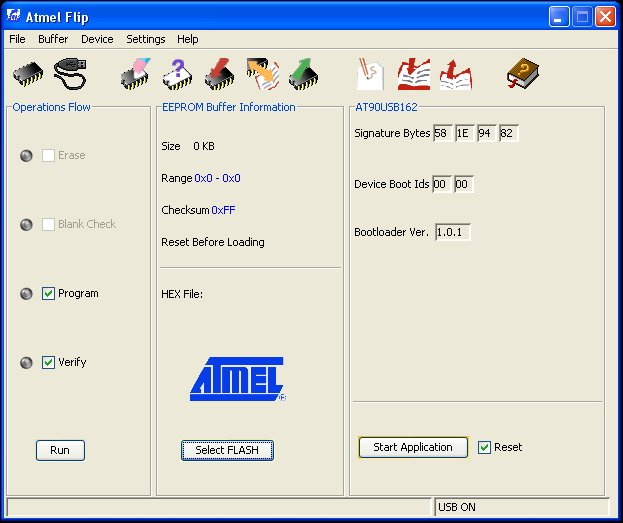
\includegraphics[width=0.6\textwidth]{images/FLIP.jpg}\\
	\rule{\linewidth}{0.5pt}
	\caption{Benuntzeroberfl�che von FLIP unter Windows}
	\label{pic:FLIP}
\end{figure}

Mit dem freien Programm \textit{DFU-Programmer} gibt es jedoch eine gute Alternative zu FLIP unter Linux. Der DFU-Programmer bietet auch die M�glichkeit den Atmega32-U4 �ber den Bootloader zu flashen. Er kann kostenlos unter http://dfu-programmer.sourceforge.net/ heruntergeladen werden.

Um das einfach anzuwendende Konsolenprogramm f�r die Verwendung mit USB zu kompilieren, wird zus�tzlich noch die Bibliothek \texttt{usblib} ben�tigt. Auch muss das Paket \texttt{automake} f�r die Erstellung des Makefiles installiert werden. Die Anwendung des Programms ist nun recht simpel. In folgendem Beispiel wird eine HEX-Datei in den Flash-Speicher des Atmega geschrieben.

\texttt{dfu-programmer atmega32u4 flash test.hex}

Der erste Parameter bezeichnet hierbei den verwendeten Mikrocontroller, der zweite die Anweisung und der dritte Parameter die zu �bertragende Datei.

Mit dem DFU-Programmer k�nnen neben den Flash-Anwendungen auch einige Fuses des Atmegas ausgelesen und gesetzt werden. Eine detailierte Beschreibung findet sich in den Manpages des Programms wieder (Linux Befehl: \texttt{man dfu-programmer}).

\section{Schnittstelle zum Logikbaustein} \label{SchnittstelleCPLD} \index{CPLD}

F�r die Kommunikation mit dem CPLD muss eine passende Schnittstelle �berlegt werden. Hardwaretechnisch sind die beiden Bausteine �ber einen 8-Bit breiten, bidirektionalen Bus, sowie 2 Steuerleitungen verbunden. Die Schnittstelle wurde im Rahmen dieser Arbeit noch nicht realisiert. In Abschnitt \ref{EntityMicro} wird eine M�glichkeit aufgezeigt, wie die Schnittstelle aufgebaut werden k�nnte.

\chapter{USB-Schnittstelle} \label{USB-Schnittstelle} % Kapitel 6

\section{Einf�hrung} \index{USB}

Die USB-Schnittstelle ist ein standartisiertes Bussystem, welches an einer vielzahl an Ger�ten verwendet wird. Die Ger�te sind meist Hot-Plug-f�hig, k�nnen also im laufenden Betrieb an die USB-Schnittstelle angeschlossen werden. In dieser Arbeit dient die USB-Schnittstelle als Verbindung zwischen dem Analysator und dem Host-PC. 

Wird ein USB-Ger�t an den PC angeschlossen, so wird es vom Betriebssystem adressiert. Danach kann mit bestimmten Registern im Ger�t, den Endpunkten, kommuniziert werden. Die Adressierung erfolgt �ber eine baumartige Strukur: Ger�t $\Rightarrow$ Konfiguration $\Rightarrow$ Interface $\Rightarrow$ Endpunkt.

Die Kommunikation kann dabei auf vier verschiedene Arten ablaufen:

\begin{description}
 \item[Kontroll-Transfer:] Dient zum Austausch von Konfigurations- und Statusdaten.
 \item[Bulk-Transfer:] Der Bulk-Transfer ist geeignet f�r gro�e Datenmengen. Dabei wird immer das gerade verf�gbare Zeitfenster verwendet
 \item[Interrupt-Transfer:] Beim Interrupt-Transfer werden Daten, welche zu unregelm��igen Zeiten vorliegen, mit voller Geschwindigkeit �bertragen
 \item[Isochrone-Transfer:] Hier werden Daten m�glichst zeitnah, also in Echtzeit �bertragen. Dabei werden, zur Analyse von Verz�gerungen, Timing-Daten mit �bertragen.
 \end{description}


\section{Hardwareschnittstelle des Atmega32-U4} \index{USB} \index{Atmega32-U4} \index{Mikrocontroller}

Der Atmega32-U4 hat, wie alle Bausteine der AT90-USB-Serie, einen USB-2.0 Baustein fest integriert. Der Baustein ist intern mit dem 8-Bit Daten- und Adressbus des AVR-Kernes verbunden. Nach au�en, zu den Anschlusspins, f�hren die Leitungen D- (Pin 3) und D+ (Pin 4). An dem Anschlusspin VBUS (Pin 7) wird die USB-Versorgungsspannung von 5V angelegt. Am Mikrocontroller ist zwar ein extra Massepin f�r den USB-Anschluss vorgesehen, jedoch ist dieser, sowohl intern als auch extern, mit der Masse der Spannungsversorgung verbunden. F�r die Unterscheidung von USB-Steckern vom Typ Micro-A- und Micro-B, kann der, bei Mikrobuchsen vorgesehene, f�nfte ID-Pin angschlossen werden. Dabei wird bei einem Micro-A Stecker der Pin auf Masse gezogen und bei einem Micro-B Stecker auf 5V. Da die Art des Steckers jedoch bei dieser Arbeit nicht relevant ist, wurde auf diesen ID-Pin verzichtet.

Da USB in der Version 2.0 mit einer Daten�bertragungsgeschwindigkeit von 12MBit/s arbeitet, ben�tigt der USB-Baustein eine Taktfrequenz von 12Mhz mit einer m�glichst hohen Genauigkeit. Da der AVR-Kern f�r Taktfreqenzen von 8MHz oder 16MHz ausgelegt ist, wird der USB-Takt direkt im Baustein erzeugt. Dazu wird der anliegende Systemtakt von 8MHz von einem PLL-Baustein \footnote{PLL: Phase-locked loop, dt: Phasenregelschleife} auf eine Frequenz von 48MHz gebracht. Diese Frequenz wird nun von einem Prescaler durch vier geteilt, wodurch die f�r den USB-Baustein n�tige Frequenz von 12MHz erzeugt wird.

Der Mikrocontroller besitzt zwar einen internen Taktgeber von 8MHz, jedoch ist dieser nicht stabil genung f�r den Betrieb des USB-Controllers. So werden die 8MHz nur bei idealen Umgebungsbedingungen stabil gehalten. Zwar ist eine externe Kompensationsschaltung m�glich, da der interne Taktgeber durch einen Registereintrag beeinflussbar ist, jedoch ist diese zu aufwendig zu realisieren. Aus diesem Grund wurde als Taktquelle ein externer Quarzoszillator verwendet, dessen Toleranzbereich kleiner ist als in der USB-Spezifikation angegeben.

Zu beachten ist, dass der interne USB-Baustein nur die elektrische Regelung des USB-Anschlusses, sowie die Anbindung an den Datenbus des AVR-Kerns �bernimmt. Im Gegensatz zu fertigen USB-Bausteinen, wie zum Beispiel ein RS232-USB Modul von FTDI, muss die Steuerung auf Protokollebene hier softwareseitig vorgenommen werden. Um jedoch nicht das komplette USB-Protokoll neu implementieren zu m�ssen, gibt es bereits fertige USB-Frameworks f�r diesen Controller. Dazu z�hlen vor allem der von Atmel selbst ver�ffentlichte USB-Stack, sowie das OpenSource Projekt LUFA. Auf diese beiden USB-Softwarel�sungen wird in den folgenden Abschnitten genauer eingegangen. 

\section{Atmel USB-Stack} \label{AtmelUSB}

\subsection{Einf�hrung} \index{Atmel USB-Stack}

Der Atmel USB-Stack stellt die Softwarebasis f�r die USB-Protokollebene zur Verf�gung. Er �bernimmt hierbei die Enumeration, also das Anmelden des USB-Devices am PC, sowie die Datenkommunikation w�hren des Betriebs. 

Mit Hilfe dieser Architektur, k�nnen Ger�te sowohl mit Low Speed (1.5 Mbit/s) als auch Full-Speed (12Mbit/s) betrieben werden. F�r Standardklassen wie zum Beispiel HID \footnote{HID: Humen Interface Device} sind bereits fertige Module implementiert. Diese k�nnen dann in die eigene Anwendung integriert werden. Als Daten�bertragunsarten sind Kontroll-, Bulk-, Isochron- und Interrupt-Transfer m�glich. F�r die Kommunikation der Anwendungssoftware mit der USB-Schnittstelle k�nnen bis zu sechs Endpunkte implementiert werden. In jeden dieser Endpunkte k�nnen bis zu zwei Puffer integriert werden, so dass der eine Puffer bereits bef�llt werden kann, w�hrend der andere noch ausgelesen wird.

In den folgenden Abschnitten wird die genaue Funktion, sowie die Anwendung des Atmel USB-Stacks erl�utert. \cite{Atmel02}

\subsection{Firmware Architektur} \index{USB-Firmware}

Die Architektur des USB-Stacks l�sst sich in vier Schichten unterteilen Auf niedrigster Ebene liegt das zu Beginn beschriebene USB-Hardwareinterface, welches durch eine Ebene dar�ber, dem Treiber, angesteuert wird. Als Schnittstelle zwischen Anwendung und Treiber dient die n�chste Schicht, die API. Diese regelt die Komunikation mit dem USB-Bus und stellt die Endpunkte zur Verf�gung. In der obersten Ebene, der Anwendungsschicht, k�nnen nun mehrere Anwendungen implementiert werden. Welche Anwendung gerade ausgef�hrt wird, regelt ein einfacher Scheduler. Somit wird die komplette Anwendung, auch die Teile welche keinen Zugriff auf den USB-Anschlus ben�tigen innerhalb dieses Schichtmodels ausgef�hrt. Bevor jedoch der Scheduler, und damit der Anwendungsteil, starten kann, m�ssen zun�chst die Initialisierungsroutinen, wie die Enumeration, ausgef�hrt werden.

\subsection{Enumeration} \label{Enumeration} \index{Enumeration} \index{Deskriptor}

Bei der Enumeration wird das USB-Ger�t beim Betriebssystem des PCs angemeldet. Daf�r fragt das Betriebssystem bestimmte Informationen vom Ger�t ab. Anhand dieser Informationen kann das Betriebssystem so den passenden Ger�tetreiber laden und dem USB-Ger�t eine Busadresse zur Kommunikation zuweisen.

Diese abrufbaren Informationen werden in USB-Diskreptoren gespeichert. Jeder dieser Diskreptoren hat seine Daten in einer Struktur gespeichert. Die Diskreptoren sind ebenfalls hirarchisch aufgebaut, und sind untereinander in einer Baumstruktur mit vier Ebenen verkn�pft (Siehe Grafik \ref{pic:Deskriptoren}). Das Ger�st der jeweiligen Datenstrukturen ist im Anhang abgebildet.

\begin{figure}[ht]
	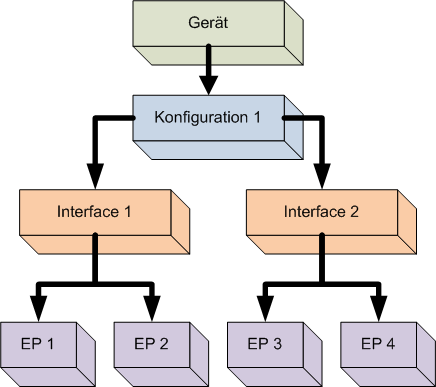
\includegraphics[width=0.6\textwidth]{images/Baumstruktur.png}\\
	\rule{\linewidth}{0.5pt}
	\caption{Baumstruktur der USB-Deskriptoren}
	\label{pic:Deskriptoren}
\end{figure}

Die Wurzel der Baumstruktur bildet der \textbf{Device-Deskriptor}. Hier sind alle grundlegenden Informationen �ber das USB-Ger�t selbst enthalten. Dazu z�hlen die verwendete USB-Version und die Ger�teklasse. Die Ger�teklasse (zum Beispiel HID-Maus) kann hier entweder fest eingetragen werden, oder, f�r Ger�te welche mehrere Klassen enthalten, in einer darunterliegenden Ebene festgelegt werden (zum Beispiel bei einem USB-Speicherstick mit integriertem Fingerabdruck-Sensor). Weitere Informationen des Device-Destkripors sind das verwendete Code-Protokoll, die Gr��e der Datenpakete und die f�r die Identifikation notwendige Vendor-, Produkt-ID und Device-ID. Zus�tzlich sind noch drei Strings vorgesehen, in welche der Hersteller, der Produktname sowie die Seriennummer im Klartext abgelegt werden k�nnen. 

Mit diesem Device-Deskriptor k�nnen nun eine oder mehrere \textbf{Konfigurations-Deskriptoren} verkn�pft werden. Hierbei ist zu beachten, dass nur eine Konfiguration aktiv sein kann. Welche dies ist, wird durch die Konfigurationsauswahl des Betriebssystems bestimmt. Im Konfigurations-Deskriptor wird die Anzahl der verwendeten Interfaces festgelegt. Au�erdem wird hier bestimmt, ob das USB-Ger�t eine eigene Spannungsversorgung besitzt oder �ber den USB-Bus versorgt wird. Wird das Ger�t �ber den USB-Bus versorgt, so wird hier auch die maximale Stromaufnahme angegeben.

Eine Ebene tiefer werden nun die \textbf{Interface-Deskriptoren} festgelegt. Hier kann nun die USB-Klasse festgelegt werden, falls diese noch nicht im Device-Desktriptor angegeben ist. Auch kann ein String abgelegt werden, um das Interface genauer zu beschreiben. Die Anzahl der, an das jeweilige Interface angeschlossenen Endpunkte, wird ebenfalls angegeben.

In der untersten Ebene der Baumstruktur sind nun die \textbf{Endpunkt-Deskriptoren} angesiedelt. Die Endpunkte bilden die eigentliche Schnittstelle zwischen der Anwendungssoftware und dem USB-Bus. Jedem Endpunkt wird in diesem Deskriptor eine 8-Bit gro�e Adresse zugewiesen, �ber welche das Betriebssystem mit dem Endpunkt direkt kommunizieren kann. Im Atmel USB-Stack k�nnen die vier niederwertigsten Bits f�r die Adressierung verwendet werden. Dies erm�glicht einen Adressbereich von 0x00 bis 0x0A. Das Bit mit dem h�chsten Stellenwert bestimmt die Richtung in der der Endpunkt betrieben wird. Somit ergibt sich f�r einen Endpunkt in OUT Richtung eine Adresse von 0x0X und f�r IN eine Adresse von 0x8X. Die �bertragungsart wird mit dem Transfer-Attribut festgelegt. Dadurch wird zwischen Kontroll, Isochron, Bulk und Interrupt-Transfer unterschieden. Die maximale Gr��e der Datenpakete, und damit die Puffergr��e, wird ebenfalls f�r jeden Endpunkt individuell bestimmt. Das letzte Attribut ist die Abtastrate des Endpunktes. Diese ist zwischen 1ms und 255ms einstellbar, wird jedoch nur bei Interrupt- und Isochrone-Transfer angewendet.

Die Datenstrukturen werden befinden sich in den Quellcodedateien \texttt{usb\_descriptor.h} und \texttt{usb\_descripor.c}. Wie neue Deskriptoren und Endpunkte erzeugt werden, ist in Abschnitt \ref{USB-Dev} genauer erl�utert.

\subsection{USB-Treiber} \index{USB-Treiber}

Der USB-Treiber bildet die Verbindung zwischen der Hardware und der Benutzerschnittstelle (API). Er enth�lt alle Low-Level Routinen, welche f�r den Betrieb des USB-Bausteins notwendig sind. Diese Routinen m�ssen normalerweise nicht f�r eigene Zwecke angepasst werden, dabBenutzerspezifische Zugriffe eine Ebene h�her, in der API, erfolgen. Beispiele f�r die im Treiber enthaltenen Routinen sind die Initialisierung und Auswahl eines Endpunktes, das Senden oder Empfangen von Daten an diesem Endpunkt, sowie das Deaktivieren und R�cksetzen. Au�erdem sind eine Vielzahl an Makros enthalten, welche die Kommunikation auf Bitebene mit dem USB-Baustein erleichtern. Als Beispiel kann hier das folgende Makro aufgezeigt werden:

\begin{quote}
%\texttt{\#define Is\_usb\_endpoint_enabled() ((UECONX \& (1 $\langel\langel$ EPEN)) ? TRUE : FALSE)}
\verb|#define Is_usb_endpoint_enabled()	((UECONX & (1<<EPEN)) ? TRUE : FALSE)|
\end{quote}

Hier wird auf Bitebene ein bestimmtes Register des USB-Bausteins abgefragt, ob der ausgew�hlte Endpunkt aktiviert ist. Als R�ckgabewert wird hier TRUE oder FALSE ausgegeben. Die in den Quellcode-Dateien \texttt{usb\_drv.h} und \texttt{usb\_drv.c} enthaltenen Makros und Low-Level-Funktionen k�nnen nun in der API angewendet werden, um h�here Funktionen zu realisieren.

\subsection{API} \index{API}

In der API werden die Funktionen bestimmt, auf welche die eigentliche Anwendung zugreift. Dadurch muss die Anwendungssoftware nicht auf die Lowlevel-Funktionen des Treibers zugreifen. Die API selbst kann nun wieder in vier Abschnitte unterteilt werden. Dazu geh�ren die Standard-USB-Funktionen. Diese Funktionen steuern alle Anfragen, welche f�r alle Klassen und Ger�te g�ltig sind und ben�tigt werden. Deshalb sollten diese Funktionen nicht ge�ndert werden. Anfragen welche nur an die verwendete Ger�teklasse gerichtet sind, werden von den ger�tespezifischen Funktionen ausgef�hrt. Dazu z�hlt zum Beispiel eine Funktion zum Senden eines Bytes �ber einen virtuellen COM-Port.

Ebenfalls zur API-Schicht werden die weiter oben beschriebenen Deskriptor-Dateien gez�hlt. Das hat den Grund, da diese bei der Initialisierung des Ger�tes von der Enumerationsroutine an den Treiber �bergeben werden.

Der vierte Abschnitt der API sind die benutzerspezifischen Funktionen. Hierzu werden alle Funktionen gez�hlt, welche nur von der Anwendungssoftware selbst verwendet werden.


\subsection{Anwendungsteil} \index{Anwendungsschicht}

Im Anwendungsteil befinden sich nun die eigentlichen Programme, welche als getrennte Tasks auf dem Prozessor ausgef�hrt werden. Zu diesen Tasks geh�rt auf jeden Fall der USB-Task. Dieser Task steuert alle allgemeinen und ger�tespezifischen Funktionen. Zu Beginn f�hrt dieser Task die Initialiserung der USB-Schnittstelle, unter Zuhilfenahme der Deskriptoren aus der API-Schicht, durch. Nach der Initialisierung f�hrt der Task interruptgesteuert alle USB-Funktionen, wie den Datentransfer oder Powermanagement (WakeUp, Resume, Reset), aus.

Neben diesem USB-Task k�nnen nun nahezu beliebig viele eigenen Anwendungen geschrieben werden. In diesen Tasks steuert man nun die HighLevel Funktionen. So wird hier zum Beispiel bei einer HID-Maus Implementierung die Funkton integriert, welche die Zust�nde der Maustasten abfragt, um diese dann �ber eine API-Funktion an den entsprechenden Endpunkt weiterzureichen. Auch k�nnen an dieser Stelle Tasks ausgef�hrt werden, die nicht auf die USB-Schnittstelle zugreifen, sondern zum Beispiel Daten von der seriellen Schnittstelle verarbeiten.

In dieser Arbeit werden im Anwendungsteil mindestens drei Tasks ben�tigt. Dazu z�hlen ein USB-RS232-Task f�r die Komunikation mit dem Analysator. Dieser wird in Abschnitt \ref{USB-UART} genauer beschrieben. Der Zweite Task stellt eine USB-JTAG-Verbindung zur Verf�gung. Mit Hilfe dieser Verbindung soll der CPLD ohne externen Programmieradapter konfiguriert werden. Dies wird im Kapitel \ref{USB-JTAG} erl�utert. Der dritte notwendige Task soll die Datenverbindung zwischen dem Mikrocontroller und CPLD herstellen. Das Konzept dieses Tasks wurde in Abschnitt \ref{SchnittstelleCPLD} erkl�rt.

Da der Prozessor des Atmega nur einen Task gleichzeitig ausf�hren kann, ist nun ein System notwendig welches die Tasks nacheinander ablaufen l�sst. Da hier kein Betriebssystem vorhanden ist, welches diese Aufgabe �benehmen k�nnte, wird auf einen einfachen Scheduler zur�ckgegriffen. Auf die Funktion und Anwendung des Schedulers wird im folgenden Abschnitt eingegegangen.

\subsection{Scheduler} \index{Scheduler} \index{Task}

Im Atmel USB-Stack ist ein einfacher Scheduler zum Ausf�hren von mehreren Tasks implementiert. Dieser Scheduler arbeitet nacheinander alle vorhandenen Tasks ab. Die einzelnen Tasks m�ssen dabei nach jedem Durchlauf abgeschlossen sein. Denn im Gegensatz zu vielen anderen Multi-Task-Systemen, springt der hier verwendete Scheduler nur in den n�chsten Task, wenn der vorherige beendet wurde.

Jeder Task wird in zwei Abschnitte unterteilt. Eine Initalisierungsroutine und die eigentliche Anwendung. Die Initialiserungsroutine wird beim Startvorgang einmal ausgef�hrt. Hier k�nnen zum Beispiel, bei der HID-Maus, die Mikrocontroller-Pins, an welchen die Maustasten angeschlossen sind, als Eing�nge definiert werden.

Der Scheduler selbst befindet sich in der Datei \texttt{scheduler.c} und wird nach der Initialisierung als Endlosschleife von der Main-Funktion ausgef�hrt. Um einen neuen Task zu erstellen, muss lediglich die Datei \texttt{conf\_scheduler.h} angepasst werden (Siehe Codebeispiel unten). Der Scheduler selbst muss nur angepasst werden, falls mehr als 11 Tasks ausgef�hrt werden sollen.

\begin{lstlisting}[caption={Ausschnitt aus conf\_scheduler.h}]
/*--------------- SCHEDULER CONFIGURATION --------------*/
#define SCHEDULER_TYPE          SCHEDULER_FREE
#define Scheduler_task_1_init   usb_task_init
#define Scheduler_task_1        usb_task
#define Scheduler_task_2_init   cdc_task_init
#define Scheduler_task_2        cdc_task
#define Scheduler_task_3_init   jtag_task_init
#define Scheduler_task_3        jtag_task
\end{lstlisting}

In der Quellcodedatei des jeweiligen Tasks, m�ssen dann mindestens die Funktion zur Initalisierung und der Task selbst enthalten sein. Au�erdem muss die Konfigurations-Header-Datei eingebunden werden.

\begin{lstlisting}[caption={Ausschnitt aus jtag\_task.c}]
#include "../conf/config.h"

void jtag_task_init(void)
{
	//Intialisierungsfunktionen
}

void jtag_task(void)
{
	//Taskfuntionen
}
\end{lstlisting}

\subsection{Anpassen an das TPLE-Board} \index{LED} \index{Mikrocontroller-Ports} 

F�r einen einfachen Umgang mit der Hardware des Analysators, kann eine boardspezifische Header-Datei erstellt werden. In dieser Datei werden dann alle verwendeten Defintionen und Makros eingetragen, welche auf die verwendete Hardware zutreffen.

Dazu z�hlt als Beispiel die Ansteuerung der beiden vorhandenen Status-LEDs. Daf�r wird zun�chst der entsprechende Port, in diesem Fall Port-F, initialisiert.

\begin{lstlisting}[caption={Ausschnitt aus usb\_tple.h}]
#define  LED_PORT       PORTF
#define  LED_DDR        DDRF
#define  LED_PIN        PINF
#define  LED1_BIT       PIND1
#define  LED2_BIT       PIND0
\end{lstlisting}

Nun k�nnen auch Makros zum einfachen Ansteuern der LEDs implementiert werden:

\begin{lstlisting}[caption={Ausschnitt aus usb\_tple.h}]
#define  Leds_init()    (LED_DDR  |= (1<<LED1_BIT) | (1<<LED2_BIT))
#define  Led1_on()      (LED_PORT |= (1<<LED2_BIT))
#define  Led1_off()     (LED_PORT &= ~(1<<LED1_BIT))
\end{lstlisting}

Diese Header-Datei kann nun in allen Quellcodedateien integriert werden, in denen auf die Hardware zugegriffen wird. Zus�tzlich zu der Ansteuerung der LEDs beinhaltet die Datei auch noch Definitionen und Makros der Verbindugsports f�r den Datenaustausch mit dem CPLD sowie f�r den JTAG-Port. Siehe auch Kapitel \ref{USB-JTAG}

\subsection{Erstellen eines neuen USB-Devices am Beispiel eines USB-UART-Adapters} \label{USB-Dev} \label{USB-UART} \index{USB-UART} \index{Interface} \index{Endpunkt}

In diesem Abschnitt wird nun kurz erl�utert wie ein neues USB-Device erstellt wird. Als Beispiel wird hier ein USB-UART Adapter erstellt. Zun�chst m�ssen daf�r die Deskriptoren definiert werden.

Zun�chst werden in der Quellcodedatei \texttt{usb\_descriptors.h} die Werte f�r alle Diskreptoren  der Baumstruktur definiert. Dies hat den Vorteil, dass diese Werte, trotz mehrfacher Verwendung, einfach ge�ndert werden k�nnen.

Begonnen wird hier mit der Wurzel des Baumes, dem Device-Deskriptor:

\begin{lstlisting}[caption={USB-Device-Deskriptor aus usb\_descriptors.h}]
#define USB_SPECIFICATION     0x0200		// USB 2.0
#define DEVICE_CLASS          CDC_GLOB_CLASS	// CDC class (0x0A)
#define DEVICE_SUB_CLASS      0      		// Unterklasse in Interface
#define DEVICE_PROTOCOL       0      		// Protokoll in Interface
#define EP_CONTROL_LENGTH     32
#define VENDOR_ID             0x1781		//HSA
#define PRODUCT_ID            0x0C66		//USB-TPLE
#define RELEASE_NUMBER        0x1000
#define MAN_INDEX             0x00
#define PROD_INDEX            0x00
#define SN_INDEX              0x00
#define NB_CONFIGURATION      1			// Anzahl Konfigurationen
\end{lstlisting}

Als n�chstes werden die Deskriptorwerte der Konfiguraion festgelegt. Im Normalfall wird nur eine Konfiguration ben�tigt. Es w�re jedoch an dieser Stelle m�glich eine zweite Konfiguration einzuf�gen, welche dann beim Start vom Betriebssystem des Hostrechners ausgew�hlt wird.

\begin{lstlisting}[caption={Konfigruations-Deskriptor aus usb\_descriptors.h}]
#define NB_INTERFACE       3	// Anzahl der Interface Deskriptoren
#define CONF_NB            1	// Nummer der Konfiguration	
#define CONF_INDEX         0	// Auswahlindex des Betriebssystems
#define CONF_ATTRIBUTES    USB_CONFIG_BUSPOWERED
#define MAX_POWER          250  // Maximaler Strom: 250x2mA = 500mA
\end{lstlisting}

F�r einen USB-UART-Adapter werden zwei getrennte Interfaces ben�tigt. Davon ist eines f�r die Daten�bertragung in Sende- und Empfangsrichtung verantwortlich, das andere ist f�r die Steuerung des Datenflusses zust�ndig.

\begin{lstlisting}[caption={Interface-Deskriptor aus usb\_descriptors.h}]
// Interface 0 descriptor
#define INTERFACE0_NB        0
#define ALTERNATE0           0
#define NB_ENDPOINT0         1			//Anzahl der angeschlossenen EP
#define INTERFACE0_CLASS     CDC_COMM_CLASS	//Klasse des Interfaces (0x02)
#define INTERFACE0_SUB_CLASS CDC_COMM_SUBCLASS	//Unterklasse (0x02)
#define INTERFACE0_PROTOCOL  CDC_COMM_PROTOCOL	//Protokoll (0x01)
#define INTERFACE0_INDEX     0

// Interface 1 descriptor
#define INTERFACE1_NB        1
#define ALTERNATE1           0
#define NB_ENDPOINT1         2			//Anzahl der angeschlossenen EP
#define INTERFACE1_CLASS     CDC_DATA_CLASS	//Klasse des Interfaces (0x0A)
#define INTERFACE1_SUB_CLASS CDC_DATA_SUBCLASS	//Unterklasse (0x00)
#define INTERFACE1_PROTOCOL  CDC_DATA_PROTOCOL	//Protokoll (0x00)
#define INTERFACE1_INDEX     0
\end{lstlisting}

Als letztes werden nun die Deskriptoren der Endpunkte festgelegt.

\begin{lstlisting}[caption={Interface-Deskriptor aus usb\_descriptors.h}]
// USB Endpoint 1 descriptor Bulk IN
#define TX_EP_SIZE          0x20	// Gr��e des Puffers in Byte
#define ENDPOINT_NB_1       USB_ENDPOINT_IN | TX_EP	// 0x81
#define EP_ATTRIBUTES_1     0x02	// BULK = 0x02, INTERUPT = 0x03
#define EP_SIZE_1           TX_EP_SIZE	// gleiche Gr��e wie Puffer
#define EP_INTERVAL_1       0x00
// USB Endpoint 2 descriptor Bulk OUT  RX endpoint
#define RX_EP_SIZE          0x20	// Gr��e des Puffers in Byte
#define ENDPOINT_NB_2       RX_EP	// 0x02
#define EP_ATTRIBUTES_2     0x02	// BULK = 0x02, INTERUPT = 0x03
#define EP_SIZE_2           RX_EP_SIZE	// gleiche Gr��e wie Puffer
#define EP_INTERVAL_2       0x00
// USB Endpoint 3 descriptor Interrupt IN
#define INT_EP_SIZE         0x20	// Gr��e des Puffers in Byte
#define ENDPOINT_NB_3       USB_ENDPOINT_IN | INT_EP	// 0x83
#define EP_ATTRIBUTES_3     0x03	// BULK = 0x02, INTERUPT = 0x03
#define EP_SIZE_3           INT_EP_SIZE	// gleiche Gr��e wie Puffer
#define EP_INTERVAL_3       0xFF 	// Polling Zeit: 255ms
\end{lstlisting}

Zus�tzlich k�nnen an dieser Stelle auch die String-Desktriptoren definiert werden. Als Beispiel wird hier der Hersteller-String-Desktriptor angegeben:

\begin{lstlisting}[caption={String-Deskriptor aus usb\_descriptors.h}]
#define USB_MN_LENGTH         3
#define USB_MANUFACTURER_NAME \
{ Usb_unicode('H') \
, Usb_unicode('S') \
, Usb_unicode('A') \
}
\end{lstlisting}

Nun m�ssen die Werte der Deskriptoren in die Datenstrukturen geschrieben werden. Die Prototypen der Strukturen befinden sich ebenfalls in der gleichen Header-Datei wie die Deskriptor-Werte, m�ssen jedoch nicht weiter angepasst werden. Die einzige Struktur die anzupassen ist, ist die Gesamtstruktur, welche die Endpunkt- und Interface-Desktriptoren an die Konfiguration kn�pft.

\begin{lstlisting}[caption={Konfigurations-Deskriptor-Strukur aus usb\_descriptors.h}]
typedef struct
{
   S_usb_configuration_descriptor cfg;
   S_usb_interface_descriptor     ifc0;
   S_usb_endpoint_descriptor      ep3;
   S_usb_interface_descriptor     ifc1;
   S_usb_endpoint_descriptor      ep1;
   S_usb_endpoint_descriptor      ep2;
} S_usb_user_configuration_descriptor;
\end{lstlisting}

Die Daten werden in der Datei \texttt{usb\_descriptors.c} in die jeweiligen Strukturen geschrieben. Die Werte f�r den Device-Deskriptor stehen dabei in einer eigenen Datenstruktur, da dieser nur einmal vorhanden sein kann.

\begin{lstlisting}[caption={Device-Deskriptor aus usb\_descriptors.c}]
// usb_user_device_descriptor
code S_usb_device_descriptor usb_dev_desc =
{
  sizeof(usb_dev_desc)
, DESCRIPTOR_DEVICE
, Usb_write_word_enum_struc(USB_SPECIFICATION)
, DEVICE_CLASS
, DEVICE_SUB_CLASS
, DEVICE_PROTOCOL
, EP_CONTROL_LENGTH
, Usb_write_word_enum_struc(VENDOR_ID)
, Usb_write_word_enum_struc(PRODUCT_ID)
, Usb_write_word_enum_struc(RELEASE_NUMBER)
, MAN_INDEX
, PROD_INDEX
, SN_INDEX
, NB_CONFIGURATION
};
\end{lstlisting}

Nun werden der Konfigurations-, die Interface- und die Endpunkt-Deskriptoren in die oben erw�hnte Gesamtstruktur geschrieben. Aus Platzgr�nden wird hier nur der Beginn der Struktur abgebildet. Die gesamte Struktur befindet sich im Quellcode des USB-UART-Beispiels auf der Daten-CD.

\begin{lstlisting}[caption={Konfigurations-Deskriptor-Strukur aus usb\_descriptors.c}]
// usb_user_configuration_descriptor
code S_usb_user_configuration_descriptor usb_conf_desc = {
 { sizeof(S_usb_configuration_descriptor)
 , DESCRIPTOR_CONFIGURATION
 , Usb_write_word_enum_struc(sizeof(usb_conf_desc_kbd))
 , NB_INTERFACE
 , CONF_NB
 , CONF_INDEX
 , CONF_ATTRIBUTES
 , MAX_POWER
 }
 ,	// COM-Interface
 { sizeof(S_usb_interface_descriptor)
 , DESCRIPTOR_INTERFACE
 , INTERFACE0_NB
 , ALTERNATE0
 , NB_ENDPOINT0
 , INTERFACE0_CLASS
 , INTERFACE0_SUB_CLASS
 , INTERFACE0_PROTOCOL
 , INTERFACE0_INDEX
 }
 ,	// COM-Endpunkt
 { sizeof(S_usb_endpoint_descriptor)
 , DESCRIPTOR_ENDPOINT
 , ENDPOINT_NB_3
 , EP_ATTRIBUTES_3
 , Usb_write_word_enum_struc(EP_SIZE_3)
 , EP_INTERVAL_3
 }
 ,
 \\ Hier folgen nun noch des Daten-Interface und die zugeh�rigen Endpunkte
};
\end{lstlisting}

Nun kann �ber die Low-Level-Funktionen aus dem USB-Treiber direkt auf die jeweiligen Endpunkte zugegriffen werden. So kann ein Enpunkt aktiviert und, je nach Datenrichtung, der Datenpuffer gelesen bzw. beschrieben werden. Mit diesen Low-Level-Funktionen kann nun eine API erstellt werden, welche dann zum Beispiel die Funktionen zum Senden und Empfangen �ber den virtuellen COM-Port, enth�lt. In der Anwendungsschicht kann dann wiederum �ber diese API-Funktionen mit dem Host-PC kommuniziert werden.

Auf Host-PC-Seite kann ebenfalls �ber die Low-Level-Funktionen auf das USB-Ger�t zugegriffen werden. Daf�r wird zum Beispiel die Bibliothek \texttt{ubslib} verwendet. Diese bietet die zur Kommunikation n�tigen Gegenst�cke des Atmel-USB-Treibers. Dadurch ist es m�glich, eine Anwendungssoftware zu schreiben, welche �ber den USB-Bus mit dem Ger�t kommuniziert. Dies wird in Kapitel \ref{PC-Software}, \nameref{PC-Software}, genauer beschrieben.

Auch ist es, bei Standard-USB-Klassen wie dem beschriebenen USB-UART-Adapter, m�glich, einen bereits im Betriebssystem integrierten Treiber zu verwenden. Dadurch kann auf das USB-Ger�t unter Zuhilfenahme h�herer Funktionen, wie zum Beispiel mit einem Terminalprogramm, zugegriffen werden, ohne auf die Lowlevel-Funktionen der USB-Bibliothek zur�ckgreifen zu m�ssen.

\section{LUFA USB-Stack} \index{LUFA}

\begin{figure}[ht]
	\center
	
\includegraphics[width=0.15\textwidth]{images/LUFA.png}\\
	\rule{\linewidth}{0.5pt}
	\caption{Logo des LUFA-Frameworks (Quelle: http://www.fourwalledcubicle.com) }
	\label{pic:FLIP}
\end{figure}

\subsection{Einf�hrung}

Alternativ zum oben beschrieben Atmel-USB-Stack, wurde das ``Lightweight USB Framework for AVRs'', kurz LUFA, entwickelt. Zu diesem Projekt geh�rt auch der in Kapitel \ref{Mikrocontroller_Software} beschriebene USB-Bootloader. 

Das Projekt hat es sich zur Aufgabe gemacht, ohne gr��ere Kenntnisse �ber die Technik von USB, die Schnittstelle des Atmegas verwenden zu k�nnen. Dazu wurden Treiber f�r einen Gro�teil der USB-Standard-Klassen implementiert. Die gesamte Bibliothek umfasst 25 verschieden Ger�teklassen. Davon sind 14 Device-Klassen und 10 Host-Klassen, sowie eine Klasse im Dual-Modus. Die API-Funktionen dieser Bibliothek k�nnen nun direkt in der eigenen Anwendung verwendet, oder den spezifischen Bed�rfnissen angepasst werden. Die Bibliothek wird in regelm��igen Abst�nden (ca. 3 Monate) in einer stabilen Version aktualisiert. Diese sind auf der Homepage http://www.fourwalledcubicle.com/ abrufbar.

Neben der Open-Source-Lizenz (MIT) liegt der gro�e Unterschied in der zentralen Verwendbarkeit der Bibliothek. So kann der gesamte Quelcode unver�ndert in einem Unterordner des Projektes abgelegt werden. �ber diesen Ordner kann nun von der Anwendugsseite auf das Framework zugegriffen werden. So wird die Bibliothek auch f�r mehrere USB-Klassen nur einmal ben�tigt. Die API selbst ist hierbei �bersichtlicher und strukturierter gestaltet als beim Atmel-Stack, was die Anwendung wesentlich erleichtert.

Der Umfang der Bibliothek bewirkt zugleich auch dessen Nachteil. So ist der Quellcode der Bibliothek mit 1MB Gr��e relativ umfangreich und umfasst zusammen mit den zugeh�rigen Beispielaplikationen sogar mehr als 4MB.

\subsection{Firmware Architektur} \index{LUFA-Stack}

Die Architektur �hnelt der Strukur des Atmel-Stacks. Sie besteht ebenfalls aus mehreren Schichten.

In der \textbf{Low-Level-Schicht} werden, wie in der Treiber-Schicht des Atmel-Stacks, die Hardwarefunktionen zur Verf�gung gestellt. Jedoch in wesentlich komplexerem Umfang. So enth�lt der LUFA-Stack nicht nur einfache Device-Endpunkt Funktionen, sondern auch Funktionen f�r den Hostbetrieb. Ausserdem ist mit LUFA die Entwicklung eines OTG- \footnote{OTG: On The Go} Ger�tes m�glich. Das bedeutet das ein Ger�t, etwa ein USB-Speicher, auch als eingeschr�nkter Host betrieben werden kann. So kann zum Beispiel eine Digitalkamera an diesen USB-Speicher angeschlossen werden um automatisch Fotos von dieser zu sichern. LUFA stellt an dieser Stelle auch Templates zu Verf�gung, um einen direkten Zugriff auf die Low-Level Funktionen ohne API zu erm�glichen.

F�r bestimmte Mikrocontroller und Entwicklungsboards beinhaltet LUFA auch noch Low-Level-Funktionen f�r nicht-USB-Hardware. Dazu z�hlen zum Beispiel A/D-Wandler oder die serielle Schnittstelle.

Die Funktionen der \textbf{High-Level-Schicht} erledigen Aufgaben wie zum Beispiel das Setzten der Deskriptoren beim Start und die Steuerung des USB-Buses im Betrieb. Dazu z�hlen die Interruptverwaltung, sowie die Regelung der Daten�bertragung an die Endpunkte.

Die dritte Schicht, welche mit der API-Schicht des Atmel-Stacks verglichen werden kann, ist die \textbf{Klassen-Schicht}. Hier sind nun alle h�heren Funktionen, getrennt nach Klassen, implementiert. Auf diese Funktionen kann nun von der eigentlichen Anwendung zugegriffen werden. Insgesamt sind hier 25 verschiedene Klassen implementiert, von Audio-Device bis zum virtuellen-seriellen-Host. F�r jede Klasse werden hierbei 2 Dateien verwendet, eine Quellcode-Datei, in welcher sich alle Funktionen befinden, sowie eine Header-Datei, mit den Prototypen der Funktionen und den Strukturdefinitionen. Diese Header-Datei wird nun in die Anwendung eingebunden, um auf die Klassenfunktionen zugreifen zu k�nnen.

Die \textbf{Anwendungsschicht} entspricht im Wesentlichen der im Atmel-Stack, auch hier kommt ein seperater Scheduler zum Einsatz. Alternativ k�nnen die Anwendungsfunktionen auch in einer Endlosschleife innerhalb der Main-Funktion ausgef�hrt werden. Nach jedem Durchlauf der Schleife wird die Funktion \texttt{USB\_USBTask()} ausgef�hrt. Diese High-Level Funktion ist f�r die Steuerung des USB-Busses verantwortlich. Vor dieser Endlosschleife muss zur Initialisierung des USB-Ports die Funktion \texttt{SetupHardware()} ausgef�hrt werden. 

Die Deskriptoren werden in den Dateien \texttt{Descriptors.h} und \texttt{Descriptors.c} festgelegt. Diese Dateien werden, wie die Dateien der Anwendungsschicht, ausserhalb des LUFA-Frameworks abgelegt. Dadurch muss keine Datei des Frameworks abge�ndert werden.

\subsection{Anwendung des Framworks am Beispiel eines USB-UART-Adapters} \index{USB-UART}

F�r die Erstellung eines USB-UART-Adapters werden nun lediglich f�nf zus�tzliche Dateien ben�tigt. Jeweils eine Quellcode- und Header-Datei f�r die Deskriptoren und die eigentliche Anwendung, sowie ein Makefile, in dem einige Parameter �ber die verwendete Hardware und der Pfad zum LUFA-Framework eingestellt werden m�ssen.

Zun�chst m�ssen die Deskriptoren f�r den USB-UART-Adapter definiert werden. Dazu werden in der Datei \texttt{Descriptors.h} zun�chst die Nummerierung der Endpunkte sowie die Bestimmung der Puffergr��e definiert.

\begin{lstlisting}[caption={Festlegung der Endpunkte aus Descriptors.h}]
// Endpunkt des COM-Interfaces
#define CDC_NOTIFICATION_EPNUM         2
// Endpunkt TX, Dateneingang
#define CDC_TX_EPNUM                   3	
// Endpunkt RX, Datenausgang
#define CDC_RX_EPNUM                   4	
// Gr��e des COM-Endpunktes
#define CDC_NOTIFICATION_EPSIZE        8
// Gr��e der Daten-Endpunkte
#define CDC_TXRX_EPSIZE                16
\end{lstlisting}

F�r die Funktion des CDC-Device ist eine zus�tzliche Datenstruktur notwendig. Diese Struktur beinhaltet f�r die Enumeration notwendige zus�tzliche Daten.

\begin{lstlisting}[caption={CDC-Funktions-Deskriptor aus Descriptors.h}]
#define CDC_FUNCTIONAL_DESCRIPTOR(DataSize)	\
	struct					\
	{					\
		USB_Descriptor_Header_t Header;	\
		uint8_t                 SubType;	\
		uint8_t                 Data[DataSize];	\
	}
\end{lstlisting}

Zuletzt wird, analog zum Atmel-Stack, die Gesamtstruktur der Deskriptoren festgelegt.

\begin{lstlisting}[caption={CDC-Funktions-Deskriptor aus Descriptors.h}]
typedef struct
{
	USB_Descriptor_Configuration_Header_t	Config;
	USB_Descriptor_Interface_t	CCI_Interface;
	CDC_FUNCTIONAL_DESCRIPTOR(2)	CDC_Functional_IntHeader;
	CDC_FUNCTIONAL_DESCRIPTOR(2)	CDC_Functional_CallManagement;
	CDC_FUNCTIONAL_DESCRIPTOR(1)	CDC_Functional_AbstractControlManagement;
	CDC_FUNCTIONAL_DESCRIPTOR(2)	CDC_Functional_Union;
	USB_Descriptor_Endpoint_t	ManagementEndpoint;
	USB_Descriptor_Interface_t	DCI_Interface;
	USB_Descriptor_Endpoint_t	DataOutEndpoint;
	USB_Descriptor_Endpoint_t	DataInEndpoint;
} USB_Descriptor_Configuration_t;
\end{lstlisting}

In der Datei \texttt{Descriptors.c} werden nun die Daten der Deskriptoren in die Struktur geschrieben. Auch der Device-Deskriptor wird hier festgelegt. Aus Platzgr�nden wird hier nur der Device-Deskriptor, sowie der Beginn des Konfigurations-Deskriptors aufgezeigt. Der gesammte Quellcode sowie die Vorlage zur Einstellung von allen Deskriptoren, befindet sich im LUFA-Verzeichnis auf dem Datentr�ger.

\begin{lstlisting}[caption={Device-Deskriptor und Teil aus Konfigurations-Deskriptor aus Descriptors.c}]
USB_Descriptor_Device_t PROGMEM DeviceDescriptor =
{
  .Header	= {.Size = sizeof(USB_Descriptor_Device_t), .Type = DTYPE_Device},
  .USBSpecification	= VERSION_BCD(01.10),	//USB Version 1.1
  .Class		= 0x02,		 //Klasse: CDC
  .SubClass		= 0x00,		 //Unterklasse in Konfiguration
  .Protocol		= 0x00,		 //Protokoll in Konfiguration
  .Endpoint0Size	= FIXED_CONTROL_ENDPOINT_SIZE,	//Gr��e EP 0
  .VendorID		= 0x03EB,	 // Vendor ID (Atmel)
  .ProductID		= 0x204B,	 // Produkt ID (Atmel CDC)
  .ReleaseNumber	= 0x0000,	 // Versionsnummer
  .ManufacturerStrIndex	= 0x01,		 // Hersteller-String
  .ProductStrIndex	= 0x02,		 // Produkt-String
  .SerialNumStrIndex	= NO_DESCRIPTOR, // Seriennummer-String
  .NumberOfConfigurations = 1		 // Anzahl der Konfigurationen
};

USB_Descriptor_Configuration_t PROGMEM ConfigurationDescriptor =
{
  //Konfigurations-Deskriptor
  .Config =
  {
    .Header = {.Size = sizeof(USB_Descriptor_Configuration_Header_t), .Type = DTYPE_Configuration},
    .TotalConfigurationSize = sizeof(USB_Descriptor_Configuration_t),
    .TotalInterfaces        = 2,
    .ConfigurationNumber    = 1,
    .ConfigurationStrIndex  = NO_DESCRIPTOR,
    .ConfigAttributes       = (USB_CONFIG_ATTR_BUSPOWERED | USB_CONFIG_ATTR_SELFPOWERED),
    .MaxPowerConsumption    = USB_CONFIG_POWER_MA(500)
  },
  ...
  // Interface-Deskriptor:
  .DCI_Interface =
  {
    .Header                 = {.Size = sizeof(USB_Descriptor_Interface_t), .Type = DTYPE_Interface},
    .InterfaceNumber        = 1,
    .AlternateSetting       = 0,
    .TotalEndpoints         = 2,
    .Class                  = 0x0A,
    .SubClass               = 0x00,
    .Protocol               = 0x00,
    .InterfaceStrIndex      = NO_DESCRIPTOR
  },
  // Endpunkt-Deskriptor
  .DataOutEndpoint =
  {
    .Header                 = {.Size = sizeof(USB_Descriptor_Endpoint_t), .Type = DTYPE_Endpoint},
    .EndpointAddress        = (ENDPOINT_DESCRIPTOR_DIR_OUT | CDC_RX_EPNUM),
    .Attributes             = EP_TYPE_BULK,
    .EndpointSize           = CDC_TXRX_EPSIZE,
    .PollingIntervalMS      = 0x00
  },
...
};
\end{lstlisting}

Nun kann die eigentliche Anwendung erstellt werden. Bei Verwendung des Schedulers wird dieser zun�chst in der Quellcodedatei konfiguriert. Dabei m�ssen die Tasks genauso benannt werden, wie die Funktionen vom Typ TASK, welche ausgef�hrt werden. Der Task USB\_USBTask �bernimmt hierbei die USB-Funktionen, der Task CDC\_Task beinhaltet die eigentliche Anwendung.

\begin{lstlisting}[caption={Scheduler-Task-List}]
TASK_LIST
{
  { .Task = USB_USBTask	, .TaskStatus = TASK_STOP },
  { .Task = CDC_Task	, .TaskStatus = TASK_STOP },
};
\end{lstlisting}

Die Klassenfunktionen werden mit der folgenden Konfigurationsfunktion aktiviert. Dadurch werden den gew�nschten API-Treibern die entsprechenden Endpunkte und Interfaces zugewiesen. Nach dieser Konfiguration kann auf die Klassenfunktionen zugegriffen werden.

\begin{lstlisting}[caption={Klassenkonfiguration}]
USB_ClassInfo_CDC_Device_t VirtualSerial1_CDC_Interface =
{
  .Config =
  {
    .ControlInterfaceNumber           = 0,
    .DataINEndpointNumber             = CDC_TX_EPNUM,
    .DataINEndpointSize               = CDC_TXRX_EPSIZE,
    .DataINEndpointDoubleBank         = false,
    .DataOUTEndpointNumber            = CDC_RX_EPNUM,
    .DataOUTEndpointSize              = CDC_TXRX_EPSIZE,
    .DataOUTEndpointDoubleBank        = false,
    .NotificationEndpointNumber       = CDC_NOTIFICATION_EPNUM,
    .NotificationEndpointSize         = CDC_NOTIFICATION_EPSIZE,
    .NotificationEndpointDoubleBank   = false,
  },
 };
\end{lstlisting}


Nun wird die Mainfunktion erstellt. In der Mainfunktion werden zun�chst die Initialisierungsfunktionen ausgef�hrt, um als letztes den Scheduler zu starten. Der Schedluer f�hrt dann in einer Endlosschleife die konfigurierten Funktionen aus.

\begin{lstlisting}[caption={Main-Funktion}]
int main(void)
{
	MCUSR &= ~(1 << WDRF);	//Watchdog Deaktivieren
	wdt_disable();
	LEDs_Init();		//Hardware Initialisieren
	ReconfigureUSART();
	UpdateStatus(Status_USBNotReady); //Warten bis USB Bereit
	Scheduler_Init();	//Scheduler intialisieren
	USB_Init();		//USB initialisieren
	Scheduler_Start();	//Endlosschleife Scheduler
}
\end{lstlisting}

In der eigentliche Anwendung, der Funktion CDC\_Task, wird nun auf die Klassenfunktionen der API zugegriffen. Als einfaches Beispiel werden hier nur die empfangenen Bytes an die Sende-Schnittstelle �bergeben. Somit ist zum Beispiel der am PC-Terminal getippte Buchstabe, als Echo sichtbar.

\begin{lstlisting}[caption={CDC-Task}]
TASK(CDC_Task)
{
  while (CDC_Device_BytesReceived(&VirtualSerial_CDC_Interface))
  {
    CDC_Device_SendByte(&VirtualSerial_CDC_Interface, \
    CDC_Device_ReceiveByte(&VirtualSerial_CDC_Interface));
  {
}
\end{lstlisting}

An diesem Beispiel ist sehr gut sichtbar, wie einfach nun die Klassenfunktionen in die jeweilige Anwendung eingebunden werden k�nnen. Dadurch ist auch eine Integration der USB-Schnittstelle in bereits existierende Anwendungen problemlos m�glich. So k�nnen zum Beispiel serielle Standardfunktionen einfach durch die oben vorgestellten CDC-Funktionen ersetzt werden.

Wie dieses Framework und das von Atmel f�r den Analysator angewendet werden, wird in den folgenden Kapiteln beschrieben.
\chapter{USB-JTAG Schnittstelle} 
\label{USB-JTAG}% Kapitel 7

\section{Einf�hrung} \index{JTAG} \index{USB} \index{USB-JTAG} \index{Altera-MAX-II} \index{CPLD}

Eine Hauptaufgabe dieser Arbeit war es, eine M�glichkeit zu finden, den Logikbaustein ohne externe Hardware konfigurieren zu k�nnen. Da die einzige Verbindung zwischen dem Analysator und dem PC die USB-Schnittstelle ist, muss die Konfigiration �ber diesen Anschluss erfolgen. Es soll damit m�glich sein, den vom Synthetiserungstool, in diesem Fall Quartus II von Altera, erzeugeten Datenstrom aufzuspielen. Dazu ist eine zus�tzliche PC-Software n�tig, da das Konfigurationstool von Altera nur mit bestimmten, externen Programmierger�ten verwendbar ist. 

Die Programmierschnittstelle des Altera-MAX-II-Bausteins ist eine JTAG Schnittstelle. Die genaue Funktion dieser Schnittstelle wird in Abschnitt \ref{Wasist} beschrieben. Es muss also auf dem Mikrocontroller ein Adapter implementiert werden, welcher auf einer Seite diese JTAG-Schnittstelle, und auf anderer Seite den USB-Bus ansprechen kann.

Nun gibt es zwei unterschiedliche Ans�tze dies zu verwirklichen. Die erste M�glichkeit ist es, die erzeugte Konfigurationsdatei �ber die USB-Schnittstelle an den Mikrocontroller zu �bertragen. Auf dem Mikrocontroller wird nun eine Software implementiert, welche die Konfigurationsdatei interpretiert, in einen JTAG-Datenstrom wandelt und anschlie�end �ber eine Hardwareschnittstelle an den CPLD �bertr�gt. Diese Variante wird sogar von Altera als ``Embedded-Programming'' empfohlen. Jedoch hat dieser Weg einen gro�en Nachteil: Der ben�gtigte Arbeitsspeicher des Mikrocontrollers muss mindestens so gro� sein, wie die zu interpretierende Konfigurationsdatei. Die Konfigurationsdatei des verwendeten Bausteins EPM240 hat eine Gr��e von etwa 12.4 Kbyte, und �bersteigt damit den im Mikrocontroller vorhandenen RAM von 1.5Kbyte um ein vielfaches. \cite{Alter02}

Somit ist in diesem Fall nur die zweite M�glichkeit anwendbar. Hierbei wird das Interpreterprogramm auf dem PC ausgef�hrt, welcher mehr als genug Arbeitsspeicher zur Verf�gung hat. Der erzeuge JTAG-Datenstrom wird nun transparent, �ber die USB-Schnittstelle, an den Mikrocontroller �bertragen. Dieser leitet nun, unter Verwendung einiger Steuerfunktionen, den Datenstrom an die Hardwareschnittstelle weiter. Ausserdem m�ssen die von der JTAG-Schnittstelle r�ckgesendeten Daten �ber USB an die Interpreter-Software weitergeleitet werden.

Leider konnte im Laufe dieser Arbeit aus Zeitgr�nden keine problemlose Konfigurationsverbindung hergestellt werden. Jedoch werden in den folgenden Abschnitten alle Ans�tze und Arbeitsschritte erl�utert, um in Zukunft die Konfiguration des CPLD �ber USB zu erm�glichen. 

\section{Kurze Einf�hrung zu JTAG} \label{Wasist} \index{JTAG} \index{TDI} \index{TDO} \index{TMS} \index{TCK} 

JTAG ist ein von der ``\textbf{J}oint \textbf{T}est \textbf{A}ction \textbf{G}roup'' entwickelter Standard (IEEE 1149.1) um das Debuggen, Testen und Programmieren von digitalen Schaltkreisen zu erm�glichen. Dies geschieht durch einen sogenannten ``Boundary Scan''. Dabei sind in dem Baustein mehrere Stellen definiert, von welchen Signale gelesen und gesetzt werden k�nnen. Diese Stellen beinflussen den Baustein im normalen Betrieb nicht. Im JTAG-Modus werden diese Signale in Form einer langen Kette (Pfad) bitweise weitergereicht. Dabei werden neue Daten �ber den TDI \footnote {TDI: Test Data In} -Eingang in den Baustein ``geschoben'', w�hrend die Baustein-internen Daten aus dem TDO \footnote{TDO: Test Data Out}-Ausgang ``gedr�ckt'' werden. Zur Weiterverarbeitung der Daten muss sowohl die Kettenl�nge, als auch die Bedeutung der einzelnen Bitstellen bekannt sein.

JTAG ist eine synchrone Datenschnittstelle. Das hei�t sie verf�gt �ber ein Taktsignal (TCK) mit dem die Datensignale synchronisiert werden. Gesteuert wird die Daten�bertragung �ber einen Zustandsautomaten, den TAP-Controller. Dieser Automat besitzt verschiedene Zust�nde, wie zum Beispiel ``Test L�uft'' oder ``Pause''. Jeder dieser 16 Zust�nde besitzt zwei Folgezust�nde. In welchen dieser Zust�nde beim n�chsten Takt gesprungen wird, bestimmt das TMS \footnote{TMS: Test Mode Select}-Signal. Optional ist auch eine Resetleitung vorgesehen. Dadurch kann der Baustein zum Beispiel nach dem Programmieren neu gestartet werden.

Zus�tzlich verf�gt JTAG noch �ber zwei Register. Ein Instruktions- und ein Daten-Register. �ber das Instruktionsregiser kann zum Beispiel ein Befehl f�r das Ausgeben des ID-Codes gesetzt werden. Der ID-Code des Bausteins wird dann daraufhin an das Datenregister gelegt. Dieses Datenregister kann dann wiederum �ber die Datenkette ausgelesen werden.

Es k�nnen auch die TDI und TDO Leitungen mehrerer Bausteine zu einer langen Kette zusammegeschlossen werden. Dann ist zus�tzlich jedoch, neben der L�nge der Einzelketten, auch noch die Position der einzelnen Bausteine relevant. 

Bei dem verwendeten CPLD wird die JTAG-Schnittstelle ausschlie�lich zur Konfiguration verwendet. Dazu ist der interne, flashbasierende Konfigurationsspeicher an die JTAG-Kette angeschlossen. Da der Konfigurationsspeicher parallel programmiert wird, ist in dem CPLD ein Programmieradapter vorhanden, der die JTAG-Signale in die n�tigen Datensignale wandelt. \cite{Khirm01}

\section{Hardwareverbindung zwischen Mikrocontroller und CPLD} \index{SPI}

Die vier JTAG Leitungen des CPLDs werden auf eine vierpolige Stiftleiste gef�hrt. Dadurch ist der Anschluss eines externen Programieradapters, wie dem Altera-USB-Blaster, �ber eine Kabelpeitsche m�glich. Vier Anschluss-Pins des Mikrocontrollers sind ebenfalls an eine vierpolgie Stiftleiste gef�hrt, so dass diese �ber Jumper mit der JTAG-Schnittstelle verbunden werden k�nnen. Diese vier Pins befindens sich alle an Port-B des Mikrocontrollers. Dabei wurde darauf geachtet, dass die Pins f�r TDI, TDO und TMS an die Pins des SPI-Moduls angeschlossen werden. Dadurch ist es f�r eine sp�tere Implementierung m�glich, das interne SPI-Modul f�r die Datenstrom�bertragung zu nutzen, wodurch eventuell ein Geschwindigkeitsvorteil erreicht werden kann. Eine zus�tzliche Resetleitung ist bei der JTAG-Schnittstelle des CPLD nicht vorgesehen.

F�r diese Arbeit wird der Port-B allerdings als nomaler Port, also mit direkter Verbindung zum Datenbus, verwendet. Die Pinbelegung der Schnittstelle ist in Tabelle \ref{tab:JTAGPin} aufgef�hrt.

\begin{table}[h] 
\begin{tabular}{|l|l|l|}
\hline
Pin am Mikrocontroller	& Signalname	& Pin am CPLD \\
\hline \hline
B 1 (SCLK)		& TCK		& 24 \\
\hline
B 2 (MOSI)		& TDI		& 23 \\
\hline
B 3 (MISO)		& TDO		& 25 \\
\hline
B 7			& TMS		& 22 \\
\hline
\end{tabular}
\caption{JTAG Pinbelegung}
\label{tab:JTAGPin}
\end{table}



\section{JTAG-Schnittstelle basierend auf Atmel USB-Stack}

\subsection{Einf�hrung} \index{USB-JTAG}

Auf Basis des in Kapitel \ref{USB-Schnittstelle} erl�uterten USB-Stacks von Atmel, kann nun ein USB-JTAG-Device entwickelt werden. Dazu wird das erl�uterte Beispiel des USB-UART Adapters um ein zus�tzliches Interface erweitert. Dadurch entsteht ein USB-Verbundger�t, also ein Ger�t das mehr als eine Klasse enth�lt. Die Erweiterung hat den Grund, da die virtuelle serielle Schnittstelle weiterhin f�r die Komunikation mit der Hardware zur Verf�gung stehen soll.

Auf PC-Seite kommt der USB-STAPL-Player von Altera zum Einsatz. Dieser interpretiert die Konfigurationsdatei des CPLD und wandelt sie in JTAG Signale um. Diese werden dann �ber Funktionen der Bibliothek \texttt{libusb} an die entsprechenden Endpunkte des USB-Ger�ts gesendet und dort weiterverarbeitet.

\subsection{USB-STAPL-Player von Wojciech M. Zabolotny} \index{Jam-STAPL-Player}

Auf Basis des Jam-STAPL-Players von Altera, wurde von Wojciech M. Zabolotny, Dozent am Warschauer Polytechnikum, ein USB-JTAG-Adapter entwickelt.
Dieser Adapter ist Haupts�chlich f�r die Verwendung als Programmieradapter f�r Altera Logikbausteine konzipiert. Als Hardware wurde ein PIC18F4550 Mikrocontroller mit integrierter USB-Schnittstelle verwendet. Als Firmwarebasis kam das, von Pierre Gaufillet entwickelte, PIC-USB-Framework zum Einsatz.

Dieses Framework ist jedoch v�llig inkompatibel zum Atmel-USB-Stack. Deshalb kann die Firmware f�r den Atmega32-U4 nicht angewendet werden. Jedoch k�nnen die h�heren API-Funktionen f�r den Atmel-Stack nachgebildet werden. Dadurch ist es m�glich, die von Wojciech M. Zabolotny angepasste Version des Altera-Jam-STAPL-Players, f�r die Konfiguration des CPLD zu verwenden.

\subsection{Hinzuf�gen eines neuen Interfaces} \index{Interface} \index{Endpunkt}

Der erste Schritt hierf�r ist, alle n�tigen Deskriptoren f�r einen USB-JTAG-Adapter festzulegen. Die Schritte, wie dabei vorzugehen ist, sind in Kapitel \ref{USB-Schnittstelle}, Abschnitt \ref{AtmelUSB} genauer erl�utert. 

Zun�chst wird der Device Desktriptor des USB-UART Adapters angepasst. Daf�r muss die CDC-Klasse entfernt werden, da es sich bei dem Ger�t nun nicht mehr um einen reinen USB-UART Adapter handelt. Stattdessen wird die Klasse 0x00 verwendet. Diese weist den USB-Host darauf hin, dass die Festlegung der Klasse nicht im Device-Desktriptor, sondern erst in den Interface-Deskriptoren festgelegt wird. Leider hat dies zur Folge, dass daraufhin die Standard-Klassentreiber von MS Windows die virtuelle serielle Schnittstelle nicht mehr erkennen. Daf�r muss eventuell die entsprechende .inf-Datei abge�ndert werden. F�r dieses Problem wurde noch keine zufriedenstellende L�sung gefunden. Die unter Debian (Lenny) verwendeten Klassentreiber erkennen den USB-UART Adapter auch nach der �nderung des Device-Deskriptors problemlos.
In Tabelle \ref{tab:DevDesc} sind alle Werte des neuen Device-Deskriptors aufgelistet.

\begin{table}[h] 
\begin{tabular}{|l|l|l|}
\hline
Deskriptorfeld		& Wert		& Beschreibung \\
\hline \hline
bDescriptorType		& 0x01		& Device-Deskriptor \\
\hline
bcdUSB			& 0x0200	& USB 2.0	 \\
\hline
bDeviceClass		& 0x00		& Klassenspezifikation im Interface \\
\hline
bDeviceSubClass		& 0x00		& Unterklassenspezifikation im Interface \\
\hline
bDeviceProtocol		& 0x00		& Protokollpezifikation im Interface \\
\hline
bMaxPacketSize		& 32		& Maximale Paketgr��e f�r EP0 in Byte \\
\hline
idVendor		& 0x1781	& Vendor: HS-Augsburg \\
\hline
idProduct		& 0x0C66	& Product: USB-TPLE \\
\hline
bcdDevice		& 0x1000	& Versionsnummer 1.0.0.0 \\
\hline
iManufacturer		& 0x00		& Index des Hersteller-Strings \\
\hline
iProduct		& 0x00		& Index des Produkt-Strings \\
\hline
iSerialNUmber		& 0x00		& Index des Seriennummer-Strings \\
\hline
bNumConfigurations	& 1		& Anzahl der Konfigurationen \\
\hline
\end{tabular}
\caption{Werte des Device-Deskriptors}
\label{tab:DevDesc}
\end{table}

Nun kann der Kofigurationsdeskriptor angepasst werden. Notwendige Daten sind hier vor allem die Anzahl der angeschlossenen Interfaces (hier von zwei auf drei erh�ht) und der Strombedarf. Dieser wird auf den Maximalwert von 500mA gesetzt. Auch muss die Gr��e der gesamten Datenstrukur angepasst werden. Eine Besonderheit des Atmel-CDC-Adapters ist, dass hier die f�r die CDC-Konfiguration zus�tzlich n�tigen Deskriptordaten von Hand, also au�erhalb einer Strukur, eingetragen wurden. Deshalb l��t sich die gr��e der Strukur nicht berechnen, und muss manuell eingetragen werden.

\begin{table}[h] 
\begin{tabular}{|l|l|l|}
\hline
Deskriptorfeld		& Wert		& Beschreibung \\
\hline \hline
bDescriptorType		& 0x02		& Konfigurations-Deskriptor \\
\hline
bTotalLength		& 0x005A 	& Gesamtgr��e aller Deskriptoren \\
\hline
bNumInterfaces		& 3		& Anzahl der Interfaces	 \\
\hline
bConfigurationValue	& 1		& Nummer der Konfiguration \\
\hline
iConfiguration		& 0		& Index des Konfigurations-Strings \\
\hline
bmAttributes		& 0x01		& 0: Eigenversorgung \\ 
			&		& 1: Versorgung �ber USB-Bus \\
\hline
MaxPower		& 250		& Maximaler Strom in 2mA-Schritten (500mA) \\
\hline
\end{tabular}
\caption{Werte des Konfigurations-Deskriptors}
\label{tab:KonfDesc}
\end{table}

F�r den USB-JTAG Adapter wird nun ein neues Interface erstellt. Dieses Interface kann nun, unabh�ngig von den vorhandenen Interfaces f�r die USB-UART-Schnittstelle, angesprochen werden. Da JTAG eine bidirektionale Schnittstelle ist, in diesem Fall TDI, TMS und TCK in das Ger�t und TDO zur�ck zum Host, muss das Interface auch in beide Richtungen arbeiten k�nnen. Da aber ein USB-Endpunkt nur in eine Datenrichtung arbeiten kann, m�ssen an das Interface zwei Endpunke, einen f�r den Datenempfang und einen f�r das Senden von Daten, angeschlossen werden. 

Auch wichtig ist die Einstellung der Klasse und des Protokolls. Wie oben beschrieben wurde, erfolgt die Festlegung der Klasse nun nicht mehr im Device-Deskriptor, sondern in den Interface-Deskriptoren. Da in der UBS-Spezifikation f�r JTAG weder eine Standard-Klasse noch ein Standard-Protokoll vorhanden sind, werden Klasse, Subklasse und Protokoll auf einen Wert von 0xFF eingestellt. Dadurch wird dem USB-Host signalisiert, dass kein Standardtreiber verwendbar ist und das Interface nur �ber spezielle Treiber, oder direkt �ber die USB-Bibliothek ansprechbar ist.

\begin{table}[h] 
\begin{tabular}{|l|l|l|}
\hline
Deskriptorfeld		& Wert		& Beschreibung \\
\hline \hline
bDescriptorType		& 0x04		& Interface-Deskriptor \\
\hline
bInterfaceNumber	& 2	 	& Interface 0 und 1 werden f�r USB-UART ben�tigt \\
\hline
bAlternateSetting	& 2		& Alternatives Interface, wird nicht verwendet	 \\
\hline
bNumEndpoints		& 2		& Anzahl Angeschlossener Endpunkte \\
\hline
bInterfaceClass		& 0xFF		& Anbieterspezifische Klasse \\
\hline
bInterfaceSubclass	& 0xFF		& Anbieterspezifische Unterklasse \\
\hline
bInterfaceProtocol	& 0xFF		& Anbieterspezifisches Protokoll \\
\hline
iInterface		& 0		& Index des Interface-Strings \\ 
\hline
\end{tabular}
\caption{Werte des JTAG-Interface-Deskriptors}
\label{tab:IntDesc}
\end{table}

Den Endpunkten wird nun eine der verf�gbaren Adresses zugewiesen (siehe Abschnitt \ref{Enumeration}). Dabei ist darauf zu achten, bei dem Endpunkt in Eingangsrichtung, das Adress-Bit mit der h�chsten Wertigkeit zu setzten. Dies erreicht man durch Addition von 0x80 zu der Endpunktadresse. Als Daten�bertragungsart wird der Bulk-Transfer verwendet. Dadurch k�nnen gr��ere Datenmengen pro Zeitfenster �bertragen werden, um f�r zuk�nftige Implementierungen eine gr��ere JTAG-Geschwindigkeit zu erm�glichen. Aus diesem Grund wurde auch die Registergr��e der Endpunkte auf den Maximalwert von 64 Byte gesetzt, obwohl f�r das verwendete �bertragungsverfahren 2 Byte in jede Richtung ausreichen w�rden.

\begin{table}[h] 
\begin{tabular}{|l|l|l|}
\hline
Deskriptorfeld		& Wert		& Beschreibung \\
\hline \hline
bDescriptorType		& 0x05		& Endpunkt-Deskriptor \\
\hline
bEndpointAdress		& 0x04	 	& Adresse des Endpunktes \\
\hline
bmAttributes		& 0x02		& 0x02: Bulk-Transfer \\ 
			&		& 0x03: Interrupt-Transfer \\
\hline
wMaxPacketSize		& 64		& Registergr��e in Byte \\
\hline
bInterval		& 0x00		& Abfrageintervall in ms (nicht bei Bulk) \\
\hline
\end{tabular}
\caption{Werte des JTAG-RX-Deskriptors}
\label{tab:EPRXDesc}
\end{table}

\begin{table}[h] 
\begin{tabular}{|l|l|l|}
\hline
Deskriptorfeld		& Wert		& Beschreibung \\
\hline \hline
bDescriptorType		& 0x05		& Endpunkt-Deskriptor \\
\hline
bEndpointAdress		& 0x85	 	& Adresse des Endpunktes mit Richtungsangabe (MSB = 1) \\
\hline
bmAttributes		& 0x02		& 0x02: Bulk-Transfer \\ 
			&		& 0x03: Interupt-Transfer \\
\hline
wMaxPacketSize		& 64		& Registergr��e in Byte \\
\hline
bInterval		& 0x00		& Abfrageintervall in ms (nicht bei Bulk) \\
\hline
\end{tabular}
\caption{Werte des JTAG-TX-Deskriptors}
\label{tab:EPTXDesc}
\end{table}

Sind nun alle Deskriptoren angepasst und die Strukturen entsprechend erweitert worden, kann das Ger�t f�r einen ersten Test an den Hostrechner angeschlossen werden. Bei Windows als Betriebsystem wird man nun eine Meldung �ber ein neues Ger�t bekommen, f�r das Windows keinen passenden Treiber findet. Um dieses Problem zu l�sen, kann eine .inf-Datei erzeugt werden, welche dem Betriebssystem sagt, welche Treiber verwendet werden sollen. F�r die virtuelle-serielle Schnittstelle kann hier ein Standard-Treiber verwendet werden. F�r das JTAG-Interface wird kein eigener Treiber verwendet, da dieser direkt �ber die USB-BIbliothek angesprochen wird.

Unter Linux wird die virtuelle-serielle-Schnittstelle erkannt, und in das System als Ger�t \texttt{/dev/ttyASM0} eingepflegt. �ber diese Schnittstelle kann nun mit jedem Terminalprogramm ein Byte gesendet werden, welches dann als Echo wieder am Bildschirm angezeigt wird.

Wird das Ger�t unter Linux angeschlossen, kann mit dem Befehl \texttt{dmesg} die korrekte Enumeration �berpr�ft werden. Mit dem Befehl \texttt{lsusb -v} kann nun angezeigt werden, ob alle Interfaces und Endpunkte am System angemeldet wurden.

\begin{lstlisting}[caption={Ausgabe des Befehls "dmesg"}]
[29382.928143] usb 3-1: new full speed USB device using uhci_hcd and address 3
[29383.085589] usb 3-1: config 1 interface 2 has no altsetting 0
[29383.085589] usb 3-1: configuration #1 chosen from 1 choice
[29383.089326] cdc_acm 3-1:1.0: ttyACM0: USB ACM device
[29383.092648] usb 3-1: New USB device found, idVendor=1781, idProduct=0c66
[29383.092655] usb 3-1: New USB device strings: Mfr=0, Product=0, SerialNumber=0
\end{lstlisting}

\begin{lstlisting}[caption={Ausgabe des Befehls "lsusb -v" (Ausschnitt)}]
Bus 003 Device 003: ID 1781:0c66 Multiple Vendors 
Device Descriptor:
  [---]
  idVendor           0x1781 Multiple Vendors
  idProduct          0x0c66 
  bcdDevice           10.00
  [...]
    Interface Descriptor:
      bLength                 9
      bDescriptorType         4
      bInterfaceNumber        2
      bAlternateSetting       2
      bNumEndpoints           2
      bInterfaceClass       255 Vendor Specific Class
      bInterfaceSubClass    255 Vendor Specific Subclass
      bInterfaceProtocol    255 Vendor Specific Protocol
      iInterface              0 
      Endpoint Descriptor:
        bLength                 7
        bDescriptorType         5
        bEndpointAddress     0x04  EP 4 OUT
        bmAttributes            2
          Transfer Type            Bulk
          Synch Type               None
          Usage Type               Data
        wMaxPacketSize     0x0020  1x 32 bytes
        bInterval               1
      Endpoint Descriptor:
        bLength                 7
        bDescriptorType         5
        bEndpointAddress     0x85  EP 5 IN
        bmAttributes            2
          Transfer Type            Bulk
          Synch Type               None
          Usage Type               Data
        wMaxPacketSize     0x0020  1x 32 bytes
        bInterval               1
\end{lstlisting}

\subsection{Anpassen der ger�tespezifischen Funktionen} \index{API}

Die ger�tespezifischen Funktionen, welche sich in der Datei \texttt{usb\_specific\_request.c} befinden, m�ssen nun noch f�r den JTAG-Adapter erweitert werden. So befinden sich in dieser Datei die Initialisierungsfunktionen der Endpunkte, die bei Ger�testart ausgef�hrt werden. Daf�r wird die Funktion \texttt{usb\_configure\_endpoint()} mit folgenden Attributen verwendet:

\begin{lstlisting}[caption={Initialiserung der Endpunkte}]
 usb_configure_endpoint(JTAG_RX_EP,      \
                         TYPE_BULK,     \
                         DIRECTION_OUT,  \
                         SIZE_32,       \
                         ONE_BANK,     \
                         NYET_ENABLED);

  usb_configure_endpoint(JTAG_TX_EP,      \
                         TYPE_BULK,  \
                         DIRECTION_IN,  \
                         SIZE_32,     \
                         ONE_BANK,     \
                         NYET_ENABLED);
\end{lstlisting} 

Nun werden die Endpunke noch mit der Funktion \texttt{usb\_reset\_endpoint(Endpunktadresse)} aktiviert. Weitere ger�tespezifische Funktionen sind nicht n�tig, da der Host-P,C unter Verwendung der USB-Bibliothek, direkt mit den Endpunkten kommuniziert.

\subsection{Implementieren der API-Funktionen}

Nun werden die anwendugsspezifischen Schntittstellen angepasst. Die n�tigen Funktionen sind bereits in der Firmware von W. M. Zabolotny implementiert, und m�ssen nun an die Atmel-Firmware angepasst werden. Die gr��te Anpassung muss hierbei an der Art des Datenaustausches mit den Endpunktregistern erfolgen.

Bei der verwendeten USB-Firmware f�r PIC-Mikrocontroller, werden alle Funktionen nach Endpunkten getrennt ausgef�hrt. Das hei�t f�r jeden Endpunkt existiert ein eigener Task, welcher entweder angepollt, oder Interruptgesteuert ausgef�hrt wird. Bei der Atmel-Firmware kann jedoch, durch das Schichtenmodell, von der Anwendung auf alle Endpunkte zugegriffen werden. Deshalb vermischen sich bei der PIC-Firmware die API- und Anwendungsfunktionen. Diese m�ssen nun erst voneinander getrennt werden.

Ein weiterer Unterschied ist, dass der USB-JTAG Adapter von W. M. Zabolotny f�r bis zu acht JTAG-Ketten ausgelegt ist, jedoch hier nur eine Kette vorhanden ist.

Nachfolgend sind nun die Prototypen der API-Funktionen aufgelistet und beschrieben. Sie befinden sich in der Quellcodedatei \texttt{jtag\_usb\_lib.c}.

\begin{description}
 \item[void jtag\_usb\_init(void):] In dieser Initialisierungsfunktion werden alle verwendeten Flags und Z�hler zur�ckgesetzt.
 \item[void jtag\_set\_chain(U8 chain):] Diese Funktion w�hlt die JTAG-Kette aus. Da nur eine Kette vorhanden ist, wird die Variable f�r die Auswahl immer auf ``0'' gesetzt.
 \item[void jtag\_block\_xmit(U8 *datain, short len):] In dieser Funktion k�nnen TDI, TMS und TCK gleichzeitig mehrfach �bertragen werden. Als Dateneingabe f�r TDI und TMS werden die unteren beiden Bits von \texttt{datain} verwendet. in der Variable \texttt{len} ist die Anzahl der zu �bertragenden Daten angegeben. TDO wird in deser Funktion nicht gelesen und muss daher in einer eigenen Funktion verarbeitet werden.
 \item[uchar jtag\_single(uchar datain):] Auch in dieser Funktion werden TDI, TMS und TCK gesetzt. Jedoch nicht f�r mehrere Takte, sondern nur f�r einen TCK-Zyklus. Zus�tzlich werden hier jedoch auch die TDO-Daten ausgelesen und zur�ckgegeben. Daher ist diese Funktion am besten geeignet.
 \item[void set\_XXX(uchar d):] XXX steht hier f�r TDI, TMS und TCK. Mit diesen Funktionen k�nnen die drei Signale einzeln, zum Beispiel f�r Testzwecke, gesetzt werden.
 \item[uchar get\_tdo(void):] Hier wird der Wert des TDO-Pins gelesen und als Unsigned-Char zur�ckgegeben
\end{description}

Der gesamte Quellcode ist auf der Daten-CD im Abschnitt ``Mikrocontroller Firmware'' zu finden.

\subsection{Der JTAG-Task} \index{Task}

Die Funktionen der erstellten API k�nnen nun in einer Anwendung verwendet werden. Dazu wird ein neuer Task mit dem Namen ``JTAG-Task'' erstellt. Dieser befindet sich in der Quellcodedatei \texttt{jtag\_task.c} und in der Header-Datei \texttt{jtag\_task.h}. 

Leider konnten, aufgrund der in Abschnitt \ref{Probleme} erl�uterten Probleme, die API-Funktionen nicht getestet und dadurch der Task nicht vollst�ndig implementiert werden. Deshalb wird in diesem Abschnitt auf die Anwedungsfunktionen aus der Original-Firmware von W. M. Zabolotny eingegangen. Diese m�ssen dann, nach Beseitigung der USB-Probleme, noch portiert werden.

Die Hauptaufgabe der Anwendung ist es, von der PC-Software kommende Befehle zu interpretieren, und mit den verf�gbaren API-Funktionen auszuf�hren. Die Befehle befinden sich im ersten Byte des Endpunktregisters. Die Codierung ist in Tabelle \ref{tab:Befehlsliste} aufgelistet.

\begin{table}[h] 
\begin{tabular}{|l|l|l|}
\hline
Befehl				& Codierung	& Beschreibung \\
\hline \hline
GET\_INFO			& 0x01		& Gibt den String: \\
				&		& ``USB JTAG GPL Interface 1.0'' zur�ck \\
\hline
CONFIG\_CHAIN			& 0x02		& Zum setzen von Parametern wie JTAG-Timing. \\
				&		& Wird nicht verwendet \\
\hline
SINGLE\_DATA\_WITH\_READ	& 0xAC		& Funktion jtag\_single() wird ausgef�hrt \\
\hline
BLOCK\_DATA			& 0xB0		& Funktion jtag\_block\_xmit() wird ausgef�hrt \\
\hline
BLOCK\_DATA\_WITH\_READ		& 0xC0		& Wird nicht verwendet. \\
\hline
SET\_PINS			& 0xD0		& Setzt TCK, TMS und TDI (untere 3 Bit des Befehls) \\
				&		& Gibt TDO zur�ck. \\
\hline
SELECT\_CHAIN			& 0xE0		& Auswahl der JTAG-Kette. Wird nicht verwendet \\
\hline
\end{tabular}
\caption{Befehlsliste Jam-STAPL-Player}
\label{tab:Befehlsliste}
\end{table}

\subsection{Ansprechen der Hardware-Pins}

Die Makros zum Setzen der Hardware-Pins befinden sich in der Header-Datei \texttt{usb\_tple.h} zusammen mit den anderen Schnittstellen-Makros wie zum Beispiel f�r die LEDs.
\begin{lstlisting}[caption={JTAG-Makros}]
#define	jtag_init()	(JTAG_DDR |= 0x86) //10000110

#define	Jtag_TDI_1()	(JTAG_PORT |= (1<<JTAG_TDI))
#define	Jtag_TDI_0()	(JTAG_PORT &= ~(1<<JTAG_TDI))

#define	Jtag_TCK_1()	(JTAG_PORT |= (1<<JTAG_TCK))
#define	Jtag_TCK_0()	(JTAG_PORT &= ~(1<<JTAG_TCK))

#define	Jtag_TMS_1()	(JTAG_PORT |= (1<<JTAG_TMS))
#define	Jtag_TMS_0()	(JTAG_PORT &= ~(1<<JTAG_TMS))

#define	Get_TDO()	((JTAG_PIN>>JTAG_TDO) & (1))
\end{lstlisting}

Mit Hilfe dieser Makros k�nnen die API-Funktionen mit der Hardware au�erhalb der USB-Schnittstelle kommunizieren.

\subsection{Anpassen des Altera Jam-STAPL-Player} \index{Jam-STAPL-Player}

Auf PC-Seite kommt der unter \cite{Alter02} beschriebene Jam-STAPL-Player von Altera zum Einsatz. Dieses Programm interpretiert die von Quartus-II erstellen Konfigurationsdateien und wandelt diese in JTAG-Signale um. In der Grundfunktion verwendet der Player die parallele Schnittstelle des PC als Programmierinterface, wobei die vier Signale TDI, TDO, TMS und TCK je an einem eigenen Pin anliegen. In der von W. M. Zabolotny angepassten Version, werden die Signale und die in Tabelle \ref{tab:Befehlsliste} aufgelisteten Befehle, �ber die USB-Schnittstelle an die entsprechenden Endpunkte �bertragen.

Die f�r die Verwendung des PIC-USB-JTAG-Adapters angepasste Version kann mit wenigen �nderungen an den Atmel-Stack angepasst werden. Da die Software die USB-Biblitothek \texttt{libusb} verwendet, m�ssen lediglich die verwendeten VID und PID sowie die Endpunktadressen angepasst werden.

Die Hardware-IDs befinden sich in der Datei \texttt{jtag.h} im Quellcode-Ordner des Jam-Stapl-Players.

\begin{lstlisting}[caption={Einstellung der Hardware IDs}]
#define CJ_USB_ID_VENDOR (0x1781)	\\HSA
#define CJ_USB_ID_PRODUCT (0x0C66)	\\USB-TPLE
\end{lstlisting}

Die Endpunkte m�ssen in der Datei \texttt{usb\_prog.c} angepasst werden. Daf�r m�ssen an allen Funktionen der USB-Bibliothek die Endpunkte von 1 und 2 auf 4 und 5 abge�ndert werden. Als Beispiel hier die Funktion f�r den Bulk-Transfer:

\texttt{usb\_bulk\_write(hdev, 1, select\_chain, 1, 500);}

Hier ist der zweite Parameter (1) die Endpunktadresse und muss durch eine 4 ersetzt werden. Das gleiche gilt f�r die Lesefunktion \texttt{usb\_bulk\_read()}.

Die Software kann nun mit dem beigef�gten Makefile f�r Linux kompiliert und verwendet werden. F�r Windows ist eine Kompilierung mit MinGW, einer Windows-GCC-Version, m�glich, aber nicht getestet.

\subsection{Aufgetretene Probleme} \label{Probleme}

Leider sind bei der Verwendung der angepassten Altera-USB-Firmware Probleme aufgetreten, welche im Laufe dieser Arbeit nicht gel�st werden konnten. Dies betrifft vor allem die Adressierung der Endpunkte. Wird zum Beispiel ein Byte an den JTAG-RX Endpunkt gesendet, so sollte es problemlos m�glich sein, danach ein Byte an die virtuelle serielle Schnittstelle zu �bertragen. Jedoch st�rzt das Ger�t aus nicht nachvollziehbaren Gr�nden bei dem Versuch der �bertragung ab. Das Ger�t muss dann neu gestartet, und am Host-PC neu angemeldet werden.

Eine Analyse mit \texttt{dmesg} und \texttt{lsusb -v} ergab keine sichtbaren Probleme bei der Enumerierung. Vermutlich ist die USB-UART-Firmware von Atmel nicht daf�r ausgelegt, dass ein zus�tzliches Interface im Ger�t vorhanden ist. Dies k�nnte durch die Implementierung eines Dual-Serial-Adapters umgangen werden, da hier ein zus�tzliches Interface f�r die zweite serielle Schnittstelle vorhanden ist.

\section{JTAG-Schnittstelle basierend auf LUFA USB-Stack} \index{LUFA}

\subsection{Einf�hrung}

Durch das scheitern der Implementierung des Atmel-USB-Stacks, wurde kurzfristig nach Alternativen gesucht. Am besten geeignet war hier das in Kapitel \ref{USB-Schnittstelle} beschriebene LUFA-Framework. Basierend auf diesem Framework wurde von Cahaya Wirawan bereits ein USB-JTAG Adapter implementiert \footnote{Estick: http://code.google.com/p/estick-jtag/}. In den folgenden Abschnitten m�chte ich kurz die Funktionen der Firmware aufzeigen. Ein problemloses Konfigurieren des CPLD konnte in der k�rze der Zeit jedoch nicht erreicht werden.

\subsection{Estick-Firmware} \index{Estick}

Das Estick-JTAG Projekt von Cahaya Wirawan entstand aus der Idee herraus, einen kosteng�nstigen Open-Source (MIT-Lizenz) JTAG Adapter f�r ARM-Mikrocontroller zu entwickeln. Der Adapter basiert auf der Estick Entwicklerplattform der Fachhochschule Wien \footnote{http://embsys.technikum-wien.at/index.php}. Diese Plattform in Form eines USB-Sticks, enth�lt einen Atmel-AT90USB162 Mikrocontroller dessen Anschlusspins nach au�en gef�hrt sind. An diese Anschlusspins werden dann direkt die JTAG Signale abgegriffen. Da das Projekt auf dem LUFA-Stack basiert, kann es ohne Probleme f�r den verwendeten Atmega32-U4 kompiliert werden. Da beide Mikrocontrollertypen von LUFA unterst�tzt werden, muss lediglich der MCU-Entrag im Makefile von \texttt{AT90USB162} auf \texttt{Atmega32U4} ge�ndert werden. 

Realisiert wurde das Projekt mit der LUFA Version 090605 (02.06.2009), basierend auf einer Anbieterspezifischen Klasse (0xFF). Das USB-Ger�t verf�gt �ber ein Interface mit zwei Endpunkten (Eines f�r jede Richtung). Unter Linux wird f�r die Verwendung des Ger�tes die USB-Bibliothek verwendet. F�r Windows wurde von den Entwickern eine .inf-Datei erstellt, welche die USB-Bibliothek als Treiber in das Betriebssystem einpflegt.

\subsection{Anpassen der Hardwareschnittstellen}

Da der Estick-JTAG-Adapter eine andere Pinbelegung verwendet als die USB-TPLE-Platine, muss die Firmware an dieser Stelle angepasst werden.

\begin{table}[h] 
\begin{tabular}{|l|l|l|}
\hline
JTAG-Signal	& Pinbelegung Estick	& Pinbelegung USB-TPLE \\
\hline \hline
TDI		& Port B0		& Port B2 \\
\hline
TMS		& Port B1	 	& Port B7 \\
\hline
TRST		& Port B2		& Nicht verwendet \\ 
\hline
SRST		& Port B3		& Nicht verwendet \\
\hline
TCK		& Port B4		& Port B1 \\
\hline
TDO		& Port B5		& Port B3 \\
\hline
\end{tabular}
\caption{Pinbelegung Estick-JTAG}
\label{tab:Estick}
\end{table}

Die Anpassung erfolgt in der Datei \texttt{jtah\_defs.h}. Hier sind auch zus�tzlich die Makros zur Steuerueung der beiden LEDs eingebunden worden. Die Makros f�r die Maskierung k�nnen von der Original Firmware �bernommen werden.

\begin{lstlisting}[caption={Estick Pinbelegung}]
	//jtag i/o pins
	#define JTAG_OUT PORTB
	#define JTAG_IN  PINB
	#define JTAG_DIR DDRB

	//output pins
	#define JTAG_PIN_TDI  2
	#define JTAG_PIN_TMS  7
	#define JTAG_PIN_TRST 0
	#define JTAG_PIN_SRST 0
	#define JTAG_PIN_TCK  1
	//input pins
	#define JTAG_PIN_TDO  3
\end{lstlisting}

Das einzige Problem ist nun noch, dass die beiden Bits f�r TDI und TMS an Bit 0 und Bit 1 des Port B vorgesehen sind. Bei der USB-TPLE-Platine jedoch an Bit 2 und 7. Dies hat die Folge, dass die API-Funktionen nicht einfach ein Byte, mit den beiden Signalwerten an Bit 0 und 1, an den Port senden k�nnen. Deshalb muss in den API Funktionen noch ein Verschieben der Bits an die richtige Stelle erfolgen. Die API Funktionen befinden sich in der Quellcodedatei \texttt{jtag\_functions.c}.

Nun kann das Ger�t mit dem Host-PC verbunden werden. Unter Windows m�ssen nun noch die Treiber installiert werden. Die entsprechende .inf-Datei sowie die USB-Bibliothek befinden sich auf dem Datentr�ger im Unterverteichnis \texttt{Microcontroller\_Firmware/estick\_firmware/src/WindowsDriver}. F�r Linux ist kein zus�tzlicher Treiber n�tig, da die USB-Bibliothek in der Anwednugssoftware integriert ist.

\subsection{PC-Software Open-OCD} \index{Open-OCD}

Da der Estick-JTAG-Adapter urspr�nglich f�r das Debuggen von ARM-Prozessoeren enwickelt wurde, wurde nur die freie Debug-Software Open-OCD \footnote{http://openocd.berlios.de/} f�r dessen Verwendung angepasst. Prinzipiell ist es zwar m�glich, auch mit dieser Software die JTAG-Kette des CPLD zu initialisieren und die Konfiguration durchzuf�hren, jedoch konnte diese Methode aus Zeitmangel nicht mehr durchgef�hrt werden.

\section{Weitere Entwicklung}

Um die Konfiguration des CPLD �ber USB zu erm�glichen, k�nnen nun zwei Wege eingeschlagen werden. Zum einen kann die Atmel-Firmware weiterentwickelt werden, um auf Basis des Jam-STAPL-Players von Altera die Konfiguration zu erm�glichen. Der Vorteil dieser Methode ist sicherlich, dass der Player f�r die Verwendung mit Altera Logikbausteinen entwickelt wurde und deshalb auf Seite der PC-Software am wenigsten Fehler auftreten sollten. 

Die andere M�glichkeit w�re es, auf Basis des Estick-JTAG-Adapters, eine PC-Anwendung zu implementieren, mit welcher der CPLD konfiguriert werden kann. Dazu z�hlt zum Einen nat�rlich die Anpassung des Jam-STAPL-Players auf die Estick-Funktionen. Eine andere M�glichkeit ist die Verwendung von UrJTAG \footnote{http://urjtag.org/} als PC-Software. UrJTAG ist ebenfalls f�r die Konfiguration von Logikbausteinen �ber JTAG ausgelegt. In UrJTAG ist bereits eine USB-Bibliothek integriert, da die Software auch mit Programmieradaptern wie dem USB-Byte-Blaster von Altera umgehen kann.
\chapter{PC-Software} \label{PC-Software}% Kapitel 8

\section{Einf�hrung} \index{PC-Software}

In diesem Kapitel werden L�sungen, zur Realisierung von Steuer- und Analyseprogrammen auf dem Host-Rechner, vorgestellt. Da der Analysator noch nicht vollst�ndig funktionsf�hig ist, dient dieses Kapitel zur Unterst�tzung von zuk�nftigen Projektgruppen, welche die Arbeit fortsetzen.

\section{Software zur Kommunikation mit der Hardware} \index{Betriebssystem} \index{Hot-Plug} \index{Treiber} \index{Terminal}

Die einfachste Form der Kommunikation mit der Hardware ist, �ber die bereits implementierte, virtuelle serielle Schnittstelle. �ber diese Schnittstelle k�nnen beliebige Daten byteweise zwischen den Ger�ten ausgetauscht werden.

Die Installation des virtuellen COM-Ports unterscheidet sich in den unterschiedlichen Betriebssystemen. Wird das Ger�t an einen PC mit einer aktuellen Linux-Distribution angeschlossen, so wird das Ger�t vom Hot-Plug-f�higen Kernel erkannt. Durch die Festlegung der CDC-USB-Klasse \footnote{CDC: Communication Device Class} in den Deskriptoren des Ger�tes, wird automatisch der entsprechende Treiber ausgew�hlt, und ein Ger�tepfad angelegt. Danach ist das Ger�t unter \texttt{/dev/ttyACM*/} ansprechbar. Der * steht hierbei f�r eine fortlaufende Nummer. Ist der Analysator das erste CDC-Ger�t, so lautet der Ger�tepfad \texttt{/dev/ttyACM0/}.

Auch unter Windows (ab  Version 2000) sind Standardtreiber f�r die CDC-Klasse integriert. Jedoch kann das Betriebssystem den Treiber nicht vollautomatisch dem Ger�t zuweisen. Nach erstmaligem Anschlie�en am USB-Port, fragt das Betriebssystem nach dem Speicherort f�r den Treiber. Dabei ist allerdings nicht der eigentliche Treiber gemeint, sonder eine Informationsdatei, in welcher die Verwendung des richtigen Treibers festgelegt ist. Diese .inf-Datei enth�lt dabei alle Informationen welche f�r die Erkennung notwendig sind (VID, PID usw.), sowie den Speicherort des Treibers. Eine .inf-Datei f�r das CDC-Ger�t befindet sich auf dem Datentr�ger im Verzeichnis \texttt{/PC-Software/}.

�ber diese Schnittstelle kann nun im einfachsten Fall mit einem Standard-Terminal-Programm, wie zum Beispiel Minicom unter Linux, oder dem Hyperterminal unter Windows, kommuniziert werden. Die einzustellende Baud-Rate kann hier frei gew�hlt werden, da bei der CDC-Klasse die Synchronisation automatisch abl�uft, und keine Vorgabe der �bertragungsgeschwindigkeit n�tig ist. F�r eine einfache �berpr�fung der Datenverbindung, sollte im Ger�t ein Echo implementiert werden. Dabei werden alle vom Ger�t empfangenen Zeichen wieder an das Terminal zur�ckgesendet.

\section{Steuerung �ber AT-�hnliche Befehle} \index{AT-Befehle}

Um den Analysator nun �ber ein Terminal steuern zu k�nnen, m�ssen �ber die Tastatur einzugebende Befehle m�glich sein. Am besten eignen sich dabei kurze Strings aus ASCII-Zeichen, welche durch einen einfachen Parser vom Ger�t interpretiert werden k�nnen.

Die Befehle k�nnten dabei �hnlich den Modem-AT-Befehlen aufgebaut sein. Diese beginnen immer mit dem einleitenden String \texttt{AT}, gefolgt von dem Befehl (zum Beispiel \texttt{D} f�r ``Dial'') und eventuell einem Wert (zum Beispiel die Telefonnummer). Abgeschlossen wird der Befehl durch das Senden der ASCII-Codes f�r Wagenr�cklauf (\texttt{<CR>}: 0x0D) und Zeilenvorschub (\texttt{<LF>}: 0x0A). In einem Terminalprogramm werden diese Zeichen meist durch Dr�cken der ``ENTER''-Taste gesendet.

\begin{lstlisting}[caption={AT-Befehl zum W�hlen einer Telefonnummer}]
ATD 0123456789<CR><LF>
\end{lstlisting}

Als R�ckantwort kommt im Normalfall die Zeichenfolge \texttt{OK <CR><LF>} oder eine Fehlernummer \texttt{ERROR XX <CR><LF>}. Wird ein Wert als R�ckmeldung mitgesendet, so wird dieser vor dem OK �bertragen.

Auf �hnliche Weise k�nnten nun die Steuerbefehle an den Analysator gesendet werden. Zur besseren Unterscheidung, k�nnten die Befehle mit dem Einleitungsstring \texttt{TA}, f�r Timing Analysator, beginnen. Nun kann man f�r alle n�tigen Steuerbefehle einen kurzen String festlegen, welcher vom der Mikrocontrollersoftware interpretiert wird. Als Beispiel hier ein m�glicher Befehl zum Setzen des Steuerregisters.

\begin{lstlisting}[caption={AT-Befehl zum W�hlen einer Telefonnummer}]
TASCR 0xAB<CR><LF>
\end{lstlisting}

Der Befehl steht hier f�r ``\texttt{S}et \texttt{C}ontrol \texttt{R}egister'' und den Registerwert \texttt{0xAB}.

\section{Format der Daten�bertragung nach IEEE Std 1364-2001} \label{Daten�bertragung} \index{IEEE Std 1364-2001} \index{Value Change Dump}

Nun muss noch ein geeignetes Daten�bertragunsformat f�r die Messdaten festgelegt werden. Die Messdaten befinden sich in einem eigenen Datenformat im Speicher des Analysators. Dieses Datenformat k�nnte zum Beispiel so aussehen: \texttt{<24Bit Zeitstempel><8 Messwerte>}. Diese 32-Bit k�nnte man nun, in vier Bytes unterteilt, an den PC Senden. Jedoch sind, f�r Terminal-�bertragungen, Daten im Klartext wesentlich besser geeignet als das �bermitteln von Bin�rdaten. 

Daher gibt es mit dem Standard nach IEEE 1364-2001, dem ``Value Change Dump'', ein auf ASCII-Zeichen basierendes Format, zur Speicherung und �bermittlung von digitalen Messwerten. Urspr�nglich wurde dieses Format haupts�chlich von VERILOG \footnote{Verilog: Hardwarebeschreibungssprache, �hnlich VHDL} -Simulatoren verwendet. Heute wird es, aufgrund seiner �bersichtlichen Struktur, jedoch auch in anderen Bereichen eingesetzt. \cite{IEEE001}

In diesem Datenformat werden die Messwerte, wie im Speicher des Analysators, mit einem Zeitstempel versehen. Dadurch ist ein Erzeugen des Datenformates aus den Speicherdaten ohne gr��eren Aufwand m�glich. Im Dateikopf m�ssen zun�chst einige Schl�sselw�rter festgelegt werden. Diese betreffen vor allem das Format der Messwerte und das Zeitformat. Die Schl�sselw�rter beginnen Immer mit einem \texttt{\$} und enden mit \texttt{\$end}.


\begin{lstlisting}[caption={VCD-Datei mit 8 Messleitungen}]
$date June 11, 2010 $end
$version USB-TPLE 1.0 $end
$comment 24Bit Timestamp, 8Bit Data $end
$timescale 10ns $end
$scope module logic $end
$var wire 8 % data $end
$upscope $end
$enddefinitions $end

#0
b00000000 %
#2303
b00000010 %
#56843
b10000010 %

\end{lstlisting}

Die ersten drei Zeilen sind nicht zwingend Notwendig, aber zur Archivierung der Messdaten von Vorteil. In der vierten Zeile wird das Zeitformat festgelegt. Da der Z�hler direkt mit dem 100MHz-Takt verbunden ist, ergibt sich eine zeitliche Aufl�sung von $\frac{1}{100MHz}=10ns$. In der f�nften Zeile wird das Datenformat festgelegt. In diesem Fall ein Modul f�r die Logikanalyse. Mit dem Befehl \texttt{\$var wire 8 \% data \$end} wird das Datenformat festgelegt. Hier eine 8-Bit breite Datenleitung mit dem Identifizierungszeichen ``\%''. An dieser Stelle k�nnten zus�tliche Datenleitungen festelegt werden. Diese m�ssen jedoch �ber ein anderes Indentifizierungszeichen verf�gen.

Nach diesen Definitionen, erfolgt nun direkt die Auflistung der Daten. Dabei wird zuerst der Zeitstempel, mit einer Vorgestellten \#, in 10ns-Schritten geschrieben. Dieser Wert kann, in dem oben erw�hnten Beispiel der Daten im Speicher, direkt aus den ersten 24-Bit des Speicherinhaltes �bernommen werden. Danach werden die f�r diesen Zeitstempel g�ltigen Daten geschrieben. Diese k�nnen als, mit den ASCII-Zeichen f�r 0 und 1 dargestellten, Bit-Werte dargestellt werden. Dabei wird den Messwerten ein ``b'' f�r Bitwert vor-, und das Indentifizierungszeichen ``\%`` nachgestellt.

Der Vorteil dieser Art der Speicherung mit Zeitstempel ist, dass die Daten nur gespeichert werden m�ssen, wenn eine Ver�nderung des Wertes vorliegt. Im Gegensatz dazu, m�ssen Daten ohne Zeistempel kontinuierlich gespeichert werden, um eine zeitliche Zuordnung zu erm�glichen.

Nun gibt es zwei M�glichketen wie die Daten an den Host-PC �bertragen werden. Entweder werden Sie direkt bei der Erzeugung an die serielle Schnittstelle geschrieben, oder erst im Speicher des Mikrocontrollers zwischengelagert, um sie als Ganzes zu �bertragen. Die zweite Methode ist jedoch durch den geringen RAM des Atmega32-U4 (1.5KByte) stark begrenzt, und wird durch den Speicher f�r die Messwerte (1MByte) um ein vielfaches �bertroffen.

\section{Software zur Verarbeitung der Logikdaten} \index{GUI} 

Nun m�ssen die an den PC �bertragenen Logikdaten weiterverarbeitet werden. Dies kann zum einen durch einen automatisierten Vorgang erfolgen, welcher in den vorhandenen Daten nach bestimmten Mustern sucht. So m�chte man zum Beispiel nur den zeitlichen Abstand zwischen zwei bestimmten Signalwechseln darstellen. Daf�r k�nnte man nun eine Interpreter f�r VCD-Dateien implementieren, der genau nach diesen Signalmustern sucht, und dann einfach die Differenz zwischen den Zeitstempeln anzeigt.

Eine andere M�glichkeit der Analyse der Messdaten, ist die grafische Darstellung der Messwerte. Ein solches Programm ist zum Beispiel die Open-Source-Software GTKWave.

\subsection{GTKWave} \index{GTKWave}

GTKWave wurde als Teil des gEDA \footnote{gEDA: GPL Electronic Design Automation} entwickelt, und erm�glicht die grafische Darstellung von zeitlichen Messwertverl�ufen. Es basiert vollst�ndig auf der grafischen Bibliothek GTK+, und ist plattform�bergreifend sowohl f�r Linux als auch Windows erh�ltlich.

Das Programm ist unter \url{http://gtkwave.sourceforge.net/} frei verf�gbar. Es bietet einige Werkzeuge zur Darstellung der Messdaten, wie zum Beispiel eine Zoomfunktion des Zeitbereiches. Somit kann eine optische Analyse der gemessenen Signale durchgef�hrt werden. Ein gro�er Vorteil von GTKWave f�r diese Arbeit, ist die M�glichket des direkten Imports von VCD-Dateien, so dass keine zus�tzliche Software zur Dateiumwandlung n�tig ist.

\begin{figure}[ht]
	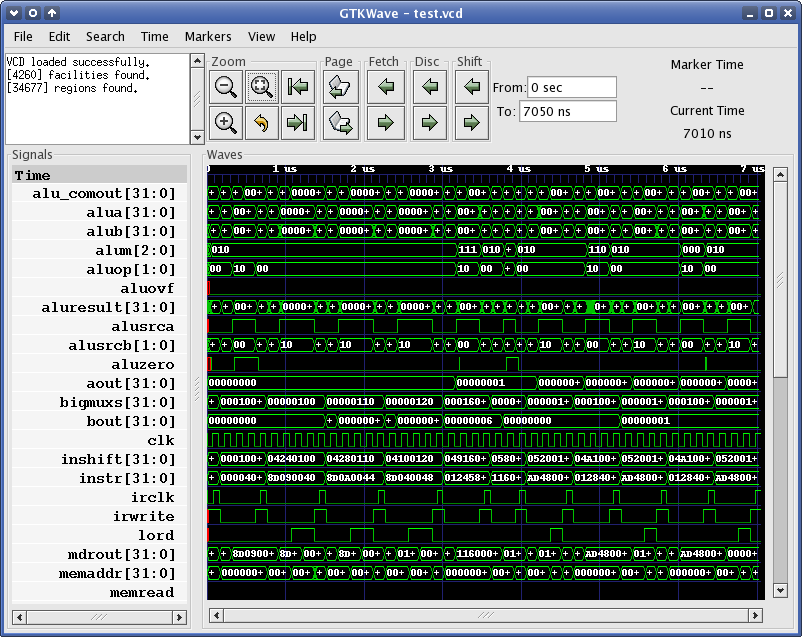
\includegraphics[width=1.0\textwidth]{images/GTKWave.png}\\
	\rule{\linewidth}{0.5pt}
	\caption{Screenshot einer komplexen Analyse in GTKWave, Quelle: wikimedia.org}
	\label{pic:GTKWave}
\end{figure}


\chapter{VHDL-Design} \label{VHDL-Design}
% Kapitel 9

\section{Einf�hrung} \index{VHDL} \index{Logikentwurf}

In diesem Kapitel werden �berlegungen zur Realisierung des Logikentwurfens aufgezeigt. Sie zeigen nur eine von vielen Implementierungen auf, und sollen nur eine Basis f�r den Aufbau des Analysators bilden. Alle hier aufgezeigten Logikschaltungen wurden nicht mehr als VHDL-Code realisiert.

Lediglich das Top-Level-Design, also die �u�erste Struktur mit allen Verbindungsleitungen nach au�en, ist bereits gegeben. Mit dieser Vorlage kann bereits mit der Implementierung begonnen werden, da allen physikalischen Anschlussleitungen bereits eine Netzname zugewiesen wurde.

\section{Entwicklungsumgebung} \index{Altera} \index{Altera-Quartus-II} \index{Modelsim} \index{USB-Blaster}

Als Entwicklungsumgebung kommt die kostenlose Web-Edition der Design-Software ``Quartus II'' von Altera zum Einsatz. Die Einschr�nkungen der kostenlosen Edition, wie zum Beispiel die fehlende IP-Core-Unterst�tzung, sind f�r den einfacheren Logikentwurf des CPLD nicht weiter relevant. 

Die aktuelle, und auch verwendete Software, ist die Version 9.1 sowohl f�r Windows und auch Linux als Host-Betriebssystem. Jedoch befindet sich die Linux-Version noch in einem Beta-Stadium. Zwar hat sich in der Verwendung der Software kein unerwarteter Fehler aufgezeigt, jedoch sind einige Enschr�nkungen in der Linux Version zu beachten. Die gr��te Einschr�nkung ist, dass das interne Simulationstool nicht verwendet werden kann. Allerdings liefert Altera als Ersatz eine kostenlose Version des Simulationstools ``Modelsim'' mit.

Die Software unterst�tzt auch den USB-Blaster als Programmierger�t. Dadurch kann direkt aus dem Designtool heraus der CPLD konfiguriert werden. F�r den sp�teren Einsatz des JAM-Stapl-Players, k�nnen mit dem Programmiertool auch SVF-Dateien erstellt werden.

\section{Top-Level-Design} \index{Top-Level-Design}

Das Top-Level-Design, also die �u�ere Struktur des Logikentwurfs verkn�pft alle implementierten Funktionseinheiten miteinander. In Grafik \ref{pic:TLD} ist eine solche Struktur abgebildet. Die Funktionen der einzelnen Funktionsbl�cke ist in den folgenden Abschnitten genauer beschrieben.

Die Pinbelegung des Bausteines wurde in der Datei \texttt{top.pin} im Verzeichnis \texttt{/PLD\_Firmware/Quartus\_project/} bereits festgelegt. Au�erdem befindet sich in diesem Vertzeichnis ein Quartus-Projekt mit einem leeren Top-Level-Design, was den Einstieg in die Entwicklung erleichtert.

\begin{figure}[ht]
	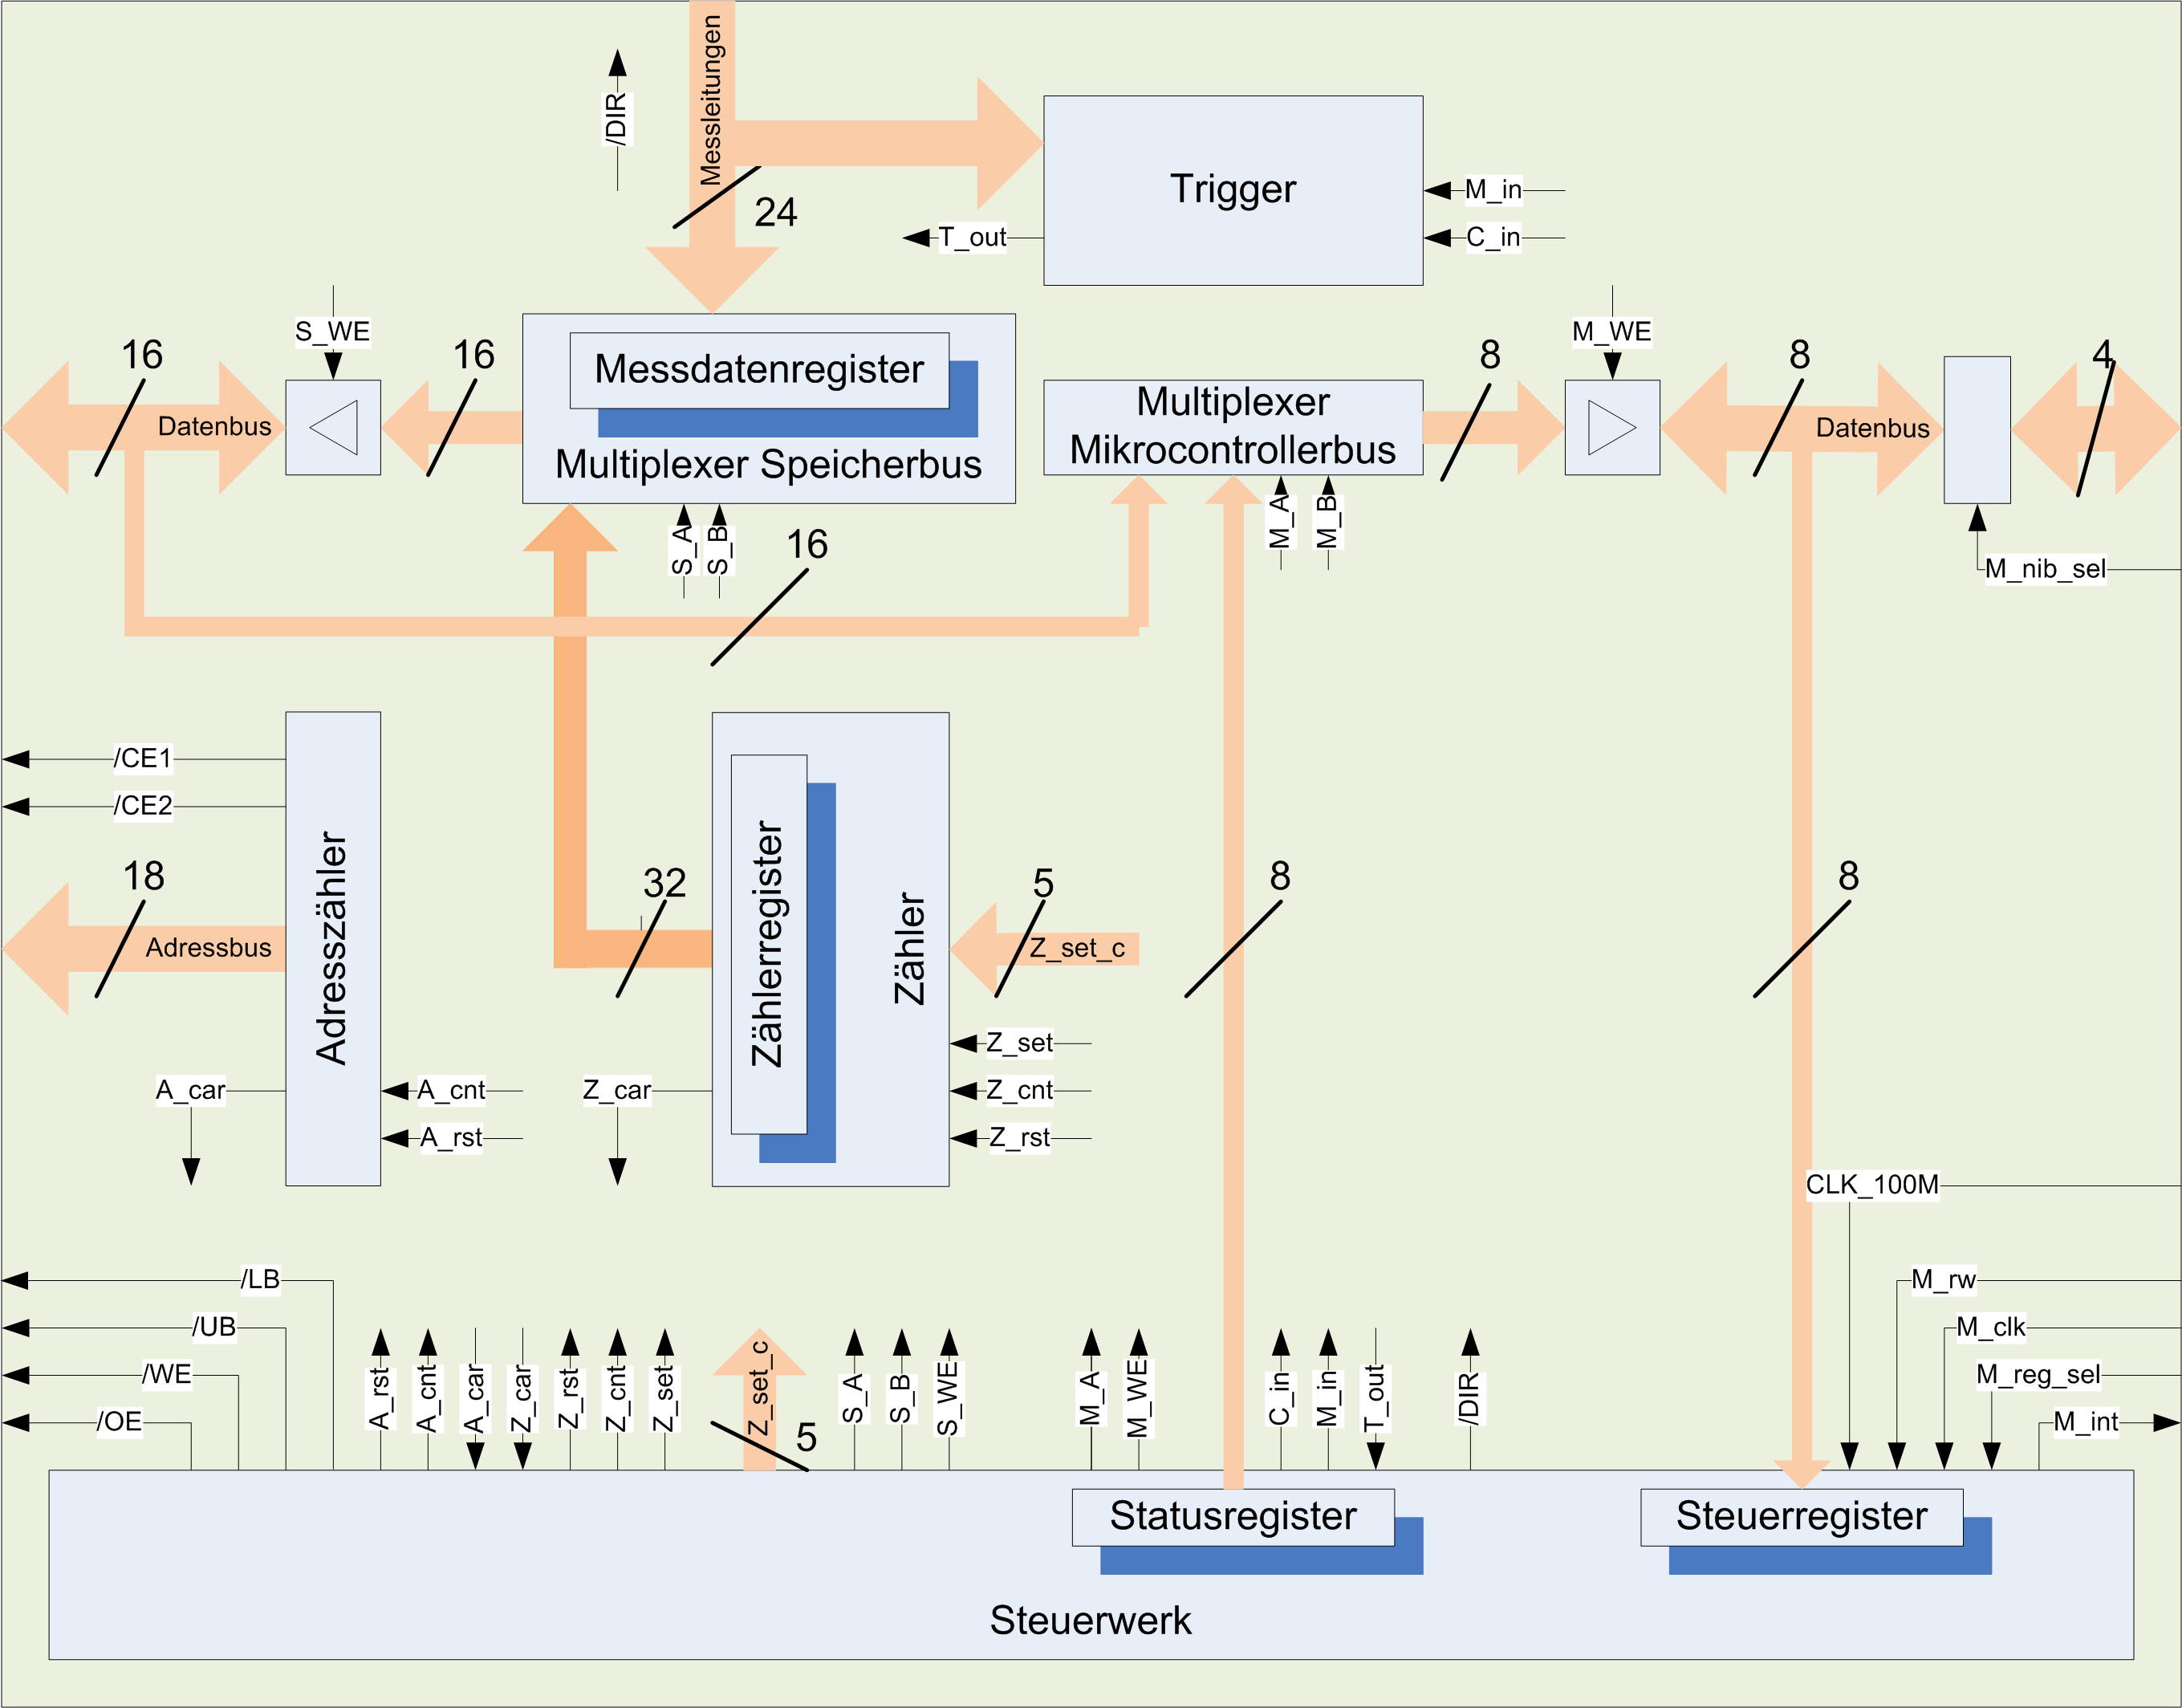
\includegraphics[width=1.0\textwidth]{images/Top_Level.png}\\
	\rule{\linewidth}{0.5pt}
	\caption{TLD eines einfachen Logikanalysators}
	\label{pic:TLD}
\end{figure}

Der hier dargestellte Entwurf erm�glicht einen Logikanalysator mit mehreren Einstellungsm�glichkeiten. So kann sowohl die Anzahl der Messleitungen, als auch die Gr��e des Zeitstempels variabel eingestellt werden. Auch ist eine Triggerung auf eine bestimmte Signalkombination m�glich. So kann die Messung automatisiert gestartet oder gestoppt werden. 

Die Ablauf wird von einem Steuerwerk geregelt. Dieses Steuerwerk besteht aus einem Zustandsautomaten, sowie zwei Registern. Eines dieser Register enth�lt die Steurbefehle vom Mikrocontroller kommend, das andere ist als Statusregister f�r die R�ckmeldung gedacht.

\begin{lstlisting}[language=VHDL, caption={Entity des Top-Level-Designs}]
--! Main Entity
entity top is
	port (
		--! External Global Signals
		clk100: in std_logic;
		ext_reset: in std_logic;
		--! Memory Interface
		mem_adr: out std_logic_vector (17 downto 0);
		mem_data: inout std_logic_vector (15 downto 0);
		mem_oe: out std_logic;
		mem_we: out std_logic;		
		mem_ce1: out std_logic;
		mem_ce2: out std_logic;
		mem_ub: out std_logic;
		mem_lb: out std_logic;
		--! ATMEGA Interface
		mega_clk: in std_logic;
		mega_int: out std_logic;
		mega_nib_sel: in std_logic;
		mega_rw: in std_logic;
		mega_reg_sel: in std_logic_vector (1 downto 0);
		mega_data: inout std_logic_vector (3 downto 0);
		--! IO-Ports
		io_dir: out std_logic;
		io_data: inout std_logic_vector (23 downto 0)	
	);
end top;
\end{lstlisting}

Bei dieser Entity, ist der Datenbus zum Atmega nochmals unterteilt in einen 4-Bit-Datenbus und f�nf Steuerleitungen. Diese Implementierung wird in Abschnitt \ref{EntityMicro} beschrieben.

\section{Trigger} \index{Trigger}

\begin{floatingfigure}[r]{0.5\textwidth}
	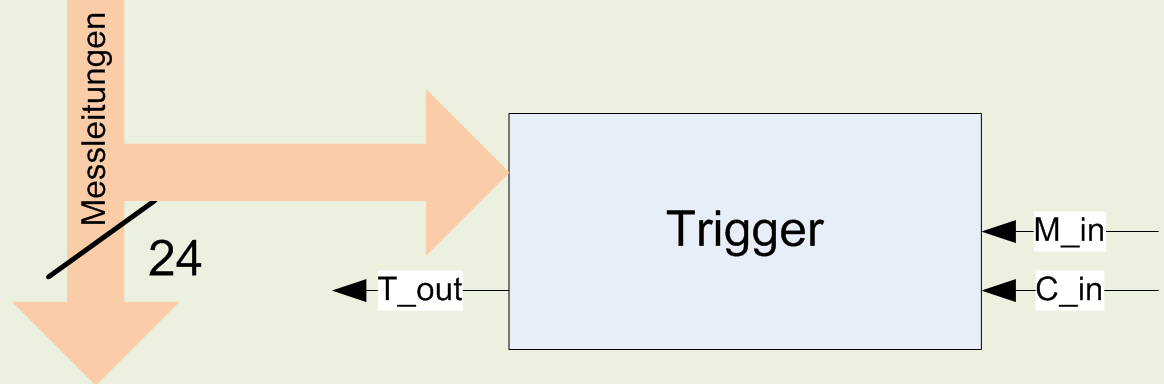
\includegraphics[width=0.4\textwidth]{images/Trigger.png}\\
	\rule{0.5\linewidth}{0.5pt}
	\caption{Blockschaltbild Trigger}
	\label{pic:Trigger}
\end{floatingfigure}

Ein Trigger ist eine Schaltung, welche bei einer bestimmten Signalkombination, oder einem bestimmten Signalwert, einen Impuls ausl�st. Mit diesem Impuls k�nnen verschiedene Ereignisse ausgel�st werden. Bei einem analogen Oszilloskop l�st der Trigger zum Beispiel beim Nulldurchgang des Signales aus, und setzt den Elektronenstrahl wieder an den linken Bildschirmrand. Dadurch entsteht ein stabiles Bild eines periodischen Signals. Bei einem Logikanalysator mit Bildschrimdarstellung kann auf eine bestimmte Signalkombination getriggert werden, um ein stabiles Bild einer periodischen Signalfolge zu erzeugen.

Der hier beschriebene Trigger hat allerdings eine etwas andere Aufgabe. Hier werden keine periodischen Signale auf einem Bildschirm dargestellt, sondern Signale �ber einen l�ngeren Zeitraum aufgezeichnet. Deshalb hat der Trigger hier die Aufgabe, den Beginn und das Ende des Speichervorgangs auszul�sen.

Dies geschieht im einfachsten Fall durch ein Signal, welches f�r den Aufnahmezeitraum auf logisch 1 gesetzt wird. Das Signal k�nnte auch gepulst sein, also jeweils f�r Start und Stopp einen kurzen Impuls ausgeben. M�glich w�ren auch zwei getrennte Leitungen f�r Start und Stop.

Der in Abbildung \ref{pic:Trigger} dargestellte Trigger ist eine wesentlich komplexere Ausbaustufe. Hierbei wird auf eine bestimmte Signalkombination aus allen 24 Messleitungen verglichen. Daf�r enth�lt dieser Trigger zwei Schieberegister und einen Vergleicher. In das erste Schieberegister wird �ber die Leitung \texttt{M\_in} eine Signalmaske geladen. M�chte man zum Beispiel nur auf die unteren acht Messleitungen triggern, so l�dt man hier \texttt{0x0000FF} als Maske. Im zweiten Register wird der eigentliche Triggerwert geladen. F�r ein wechselndes 1-0 Muster m�sste hier \texttt{0x555555} gesetzt werden. Liegt nun ein passendes Signalmuster an (zum Beipsiel \texttt{0x251B55}), so gibt der Trigger einen Impuls an das Steuerwerk weiter, welches dann alle weiteren Schritte durchf�hrt. 

\section{Speicherschnittstelle} \index{Speicherschnittstelle}

Die Speicherschnittstelle stellt die Verbindung zwischen der Logik des Analysators und dem externen Speicherbus dar. Da diese Schaltung einen �bergang von der synchronen, internen Schaltung und dem asynchronen, externen Speicher bildet, sind hier einige Details zu beachten. So muss gew�hrleistet werden, dass die Adressleitungen alle g�ltig sind, der Speicherbaustein bereits den entsprechenden Speicherabschnitt ausgew�hlt hat und die Daten am Datenbus anliegen, bevor dem Speicherbaustein das Signal zum Schreiben gegeben wird. 

Dies wird dadurch gew�hrleistet, dass die einzelnen Schritte in je einem eigenen Takt durchgef�hrt werden, wobei der Takt l�nger andauern muss, als die maximale Zugriffszeit des externen Speichers.

\subsection{Multiplexer} \index{Multiplexer}

\begin{floatingfigure}[r]{0.5\textwidth}
	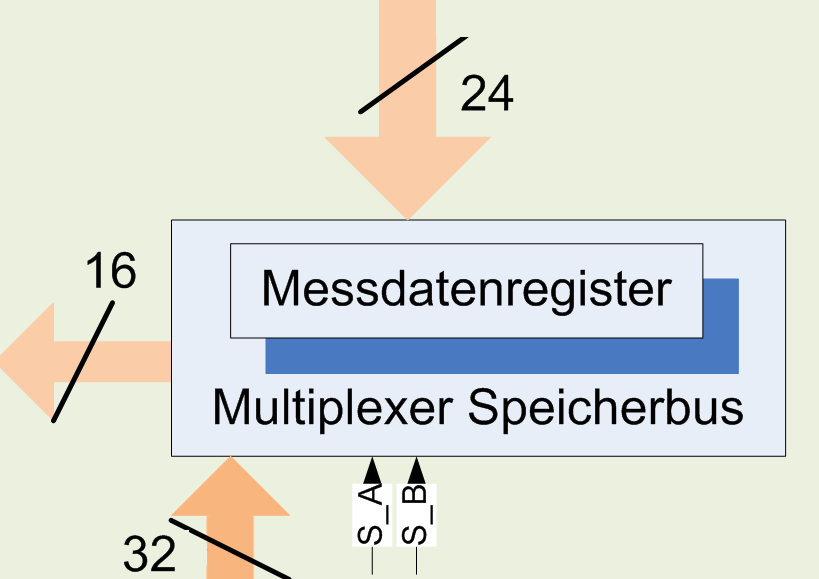
\includegraphics[width=0.4\textwidth]{images/Speichermultiplexer.png}\\
	\rule{0.5\linewidth}{0.5pt}
	\caption{Blockschaltbild Datenbus-Multiplexer}
	\label{pic:Multiplexer}
\end{floatingfigure}

Der Multiplexer f�r die Messdaten wird ben�tigt, da die Datenwortbreite des Speichers mit 16 Bit geringer ist als die Breite der Messwerde und des Zeitstempels. Deshalb muss der Multiplexer diese Signale in mehrere Worte unterteilen. 

Die maximal ben�tigte Speicherbreite sind 32 Bit Zeitstempel und 24 Bit Messdaten. F�r das Ablegen der vorliegenden 56 Bit sind also vier Speichervorg�nge n�tig. Die nicht ben�tigten 8 Bit am Ende des Speichervorgans, k�nnen entweder auf 0 belassen werden, oder f�r andere Zwecke, wie zum Beispiel einen Messwertz�hler, verwendet werden.

Der Speichervorgang ben�tigt nun also mehrere Takte. Da sich innerhalb dieser Takte der Messwert �ndern kann, muss dieser vorher in einem Messwertregister zwischengespeichert werden. F�r die Steuerung des Multiplexers sind zwei Leitungen n�tig, um einen der vier m�glichen Wege auszuw�hlen (\texttt{S\_A} und \texttt{S\_B}).

\subsection{Tristate-Treiber} \index{Tristate}

Der Datenbus zum Speicher ist als bidirektionaler Bus ausgelegt. Es werden also die selben Datenleitungen sowohl f�r das Senden, als auch f�r das Empfangen verwendet. Um hier nun einen Konflikt zu vermeiden, muss die Speicherschnittstelle (Master) dem Speicher (Slave) die Erlaubnis zum Senden von Daten geben. Dabei muss die Schnittstelle so konzipiert werden, dass sie selbst in diesem Moment nicht �ber den Datenbus sendet, da dies zum Konflikt f�hren w�rde.

Dies wird durch die Verwendung einer Steuerleitung ($\overline{WE}$) und eines Tristate-Treibers erm�glicht. Dieser schaltet, wenn der Bus vom Speicher belegt wird, den Datenausgang der Speicherschnittstelle hochohmig. Dadurch wird verhindert, dass sich beide Sendetreiber gegenseitig st�ren.

\subsection{Adressz�hler} \index{Adressz�hler}

\begin{floatingfigure}[hr]{0.4\textwidth}
	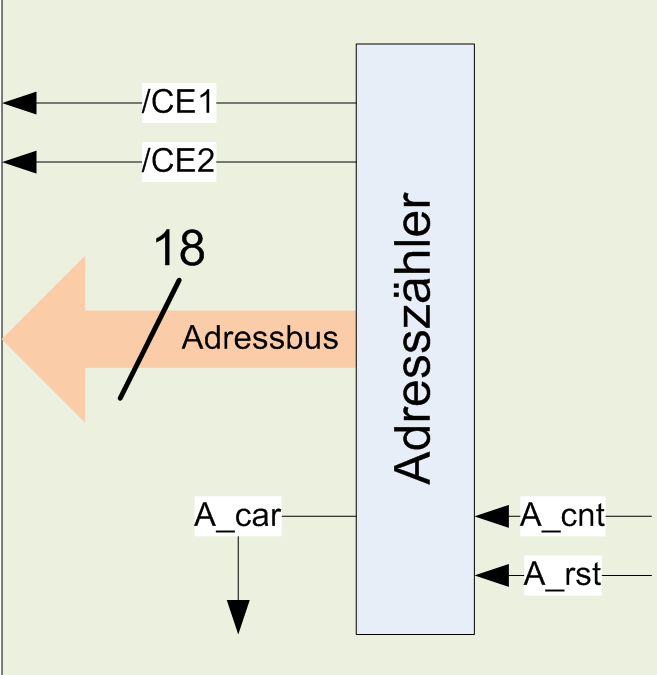
\includegraphics[width=0.2\textwidth]{images/Adresszaehler.png}\\
	\rule{0.4\linewidth}{0.5pt}
	\caption{Blockschaltbild Adressz�hler}
	\label{pic:Adresszaehler}
\end{floatingfigure}

Der Adressz�hler ist als einfacher Z�hler mit 19 Bit Breite konzipiert. Da der Z�hler sowohl im Speicher- als auch im Lesemmodus nur immer von 0 nach oben z�hlen muss, ist auch keine r�ckl�uftige Z�hlrichtung vorgesehen. Er verf�gt als Eing�nge lediglich �ber ein Reset-Signal, zur R�cksetzung auf 0, und den eigentlichen Z�hlimpuls. Dieser Z�hlimpuls wird vom Steuerwerk ausgel�st, wenn der vorherige Lese- oder Speichervorgang abgeschlossen wurde. 

Auf der Ausgansseite hat der Z�hler einen 18-Bit breiten Adressbus, welcher direkt in die Speicherbausteine gef�hrt wird. Die 19. Adressleitung wurde in die beiden Chip-Enable-Signale $\overline{CE1}$ und $\overline{CE2}$ aufgeteilt. Dies f�hrt zu einem Wechsel der Speicherbausteine, sobald die 19. Adressleitung auf 1 gesetzt wird.

F�r die Signalisierung eines �berlaufs ist eine Carry-Out Leitung vorgesehn. Diese zeigt dann dann an, dass der Speicher voll ist. Falls der Analysator nur mit einem Speicherbaustein best�ckt ist, ist darauf zu achten, das Carry-Signal schon beim Setzen der 19. Adressleitung auszugeben.

\section{Schnittstelle zum Mikrocontroller} \label{EntityMicro} \index{Mikrocontroller}

\begin{floatingfigure}[hr]{0.7\textwidth}
	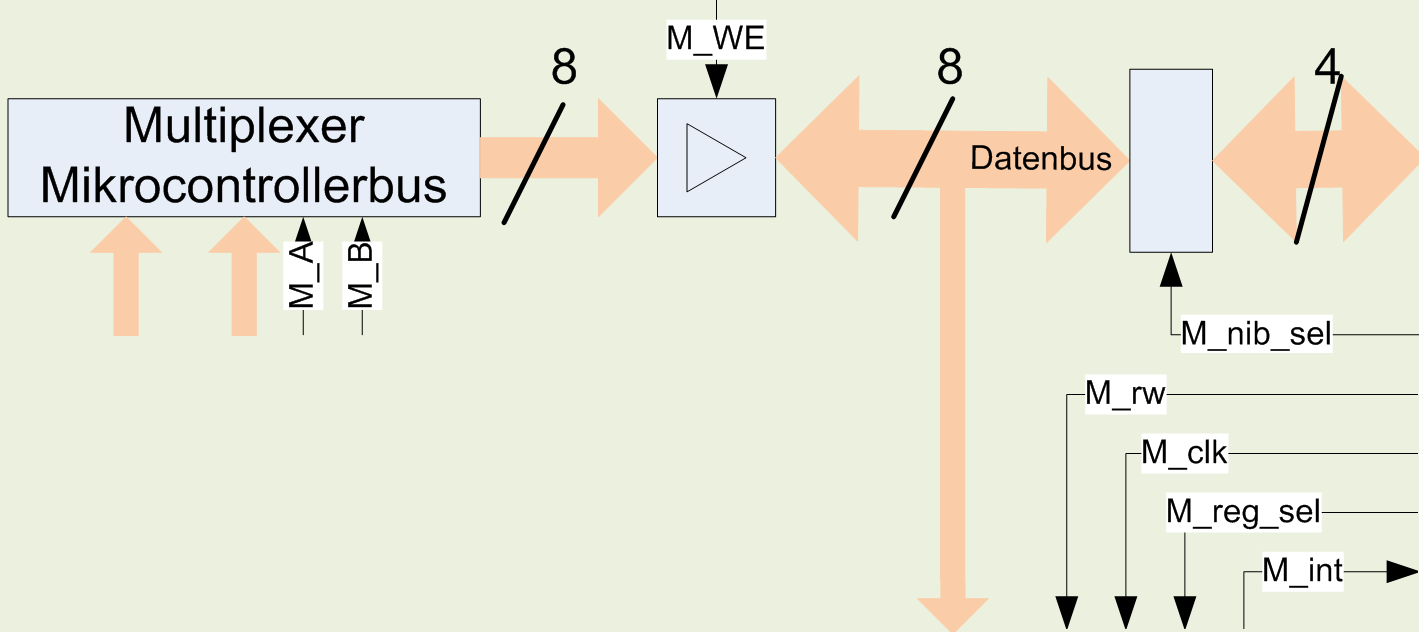
\includegraphics[width=0.6\textwidth]{images/Mikrocontroller_CPLD.png}\\
	\rule{0.7\linewidth}{0.5pt}
	\caption{Blockschaltbild der Schnittstelle zum Mikrocontroller}
	\label{pic:Timer}
\end{floatingfigure}

Die Schnittstelle zwischen Mikrocontroller und CPLD ist wesentlich komplexer als die Speicherschnittstelle. Das Hauptproblem ist, dass die Schnittstelle nicht asynchron arbeitet, sondern synchron, allerdings mit zwei unterschiedlichen Taktdom�nen. W�hrend der CPLD mit einem Takt von 100MHz arbeitet, verwendet der Mikrocontroller einen Takt von 8MHz. 

Deshalb m�ssen die Signale einsynchronisiert werden. Dies kann �ber einen synchronisierten FIFO-Puffer \footnote{FIFO: First In - First Out dt.: Erster rein - Erster raus}, bestehend aus mehreren Flip-Flops, erfolgen. Dadurch bleiben die beiden Taktdom�nen getrennt, und k�nnen sich nicht durch unterschiedliche Taktflanken gegenseitig st�ren.

Eine andere M�glichkeit w�re es, den gesamten CPLD, w�hrend des Zugriffs durch den Mikrocontroller, mit einem externen Takt laufen zu lassen. Dieser Takt k�nnte vom Mikrocontroller gesteuert werden. Bei der Wahl des Taktes w�re dann nur noch auf die Signallaufzeiten zwischen den Bausteinen zu achten.

Hardwaretechnisch verf�gt die Schnittstelle �ber einen 8-Bit breiten bidirektionalen Datenbus, sowie �ber eine Taktleitung vom Mikrocontroller kommend, und eine Interruptleitung vom CPLD kommend.

Um nun ein einfaches Protokoll zu implementieren, kann nun die Datenleitung nochmals unterteilt werden. Siehe Tabelle \ref{tab:Mic_dir}.

\begin{table}[h] 
\begin{tabular}{|l|l|l|}
\hline
Signalname	& Breite in Bit	& Richtung \\
\hline \hline
Daten		& 4		& Mikrocontroller $\Leftrightarrow$ CPLD  \\
\hline
M\_nib\_sel	& 1		& Mikrocontroller $\Rightarrow$ CPLD  \\
\hline
M\_rw		& 1		& Mikrocontroller $\Rightarrow$ CPLD  \\
\hline
M\_reg\_sel	& 2		& Mikrocontroller $\Rightarrow$ CPLD  \\
\hline
M\_clk		& 1		& Mikrocontroller $\Rightarrow$ CPLD  \\
\hline
M\_int		& 1		& Mikrocontroller $\Leftarrow$ CPLD  \\
\hline
\end{tabular}
\caption{Datenleitungen zwischen Mikrocontroller und CPLD}
\label{tab:Mic_dir}
\end{table}

Da die Daten Byteweise �bertragen werden sollen, ist das Signal \texttt{M\_nib\_sel} n�tig. Es w�hlt, aus welches Nibble \footnote{Nibble: 4-Bit-breites Datenwort} des Bytes gerade am 4-Bit breiten Datenbus anliegt. Mit der Steuerleitung \texttt{M\_rw} wird gew�hlt, ob gerade auf die Register geschrieben wird, oder von Ihnen gelesen. Mit den \texttt{M\_reg\_sel}-Leitungen wird ausgew�hlt, welches Register gerade am Datenbus anliegt. Zum Lesen k�nnen hier das Statusregister, sowie das obere oder untere Byte des Datenbuses zum Speicher, ausgew�hlt werden. Im Schreibmodus kann hier nur das Steuerregister angew�hlt werden.

F�r die Synchronisation der beiden Bausteine ist die Taktleitung \texttt{M\_clk} vorhanden. Mit der Steuerleitung \texttt{M\_int} kann der CPLD im Mikrocontroller einen Interrupt ausl�sen. Damit wird im Mikrocontroller zum Beispiel angezeigt, dass Daten zur Abholung bereit liegen.

\section{Timer} \index{Timer} \index{Z�hler}

\begin{floatingfigure}[hr]{0.4\textwidth}
	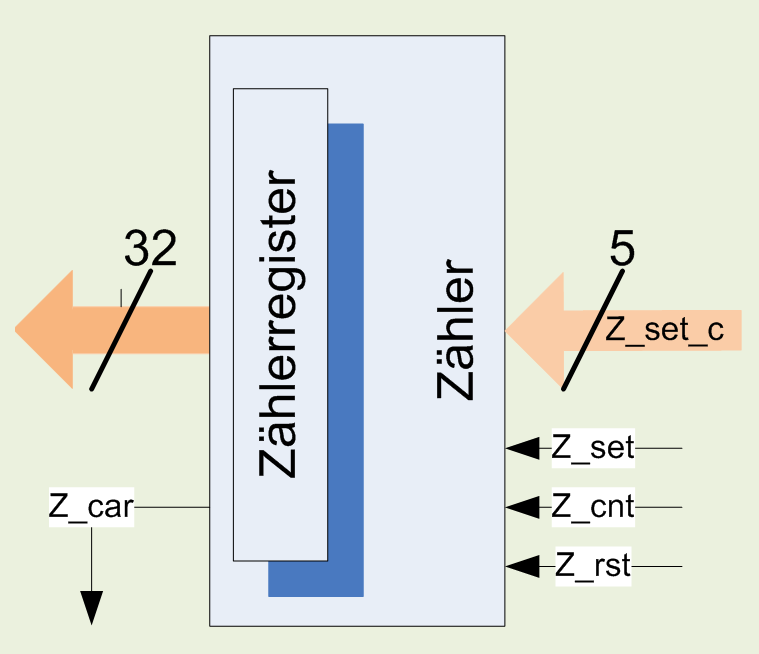
\includegraphics[width=0.3\textwidth]{images/Timer.png}\\
	\rule{0.4\linewidth}{0.5pt}
	\caption{Blockschaltbild Timer}
	\label{pic:Timer}
\end{floatingfigure}

Der Timer besteht aus einem 32-Bit-Z�hler, welcher immer mit dem genauen 100MHz Systemtakt nach oben z�hlt. Aktiviert wird er vom Steuerwerik �ber die Leitung \texttt{Z\_cnt} und zur�ckgesetzt �ber die Leitung \texttt{Z\_rst}. Soll nun ein Z�hlerwert als Zeitstempel in den Speicher geschrieben werden, so wird �ber das Signal \texttt{Z\_set} der aktuelle Z�hlerwert in das Z�hlerregister abgelegt. Nun kann dieser Wert in den Speicher geschrieben werde, w�hren der Z�hler im Hintergrund weiter mit dem Systemtakt nach oben z�hlt.

Kommt es zu einem Z�hler�berlauf, so geht das Carry Signal auf 1. Wann dieser �berlauf stattfindet, kann durch das Eingangssignal \texttt{Z\_set\_c} festgelegt werden. Damit wird ein Multiplexer gesteuert, welcher eine der 32 Z�hlerleitungen, als Carry ausw�hlt. Dies kann zum Beispiel daf�r verwendet werden, wenn nur ein 16-Bit Zeitstempel verwendet wird, um Speicherplatz zu sparen.

\section{Steuerwerk} \index{Steuerwerk}

Das Steuerwerk ist f�r die Abl�ufe in dem Analysator zust�ndig. Es sollte als synchroner Automat konzipert werden. Als Ausg�nge verf�gt das Steuerwerk �ber s�mtliche Steuerleitungen der einzelnen Komponenten, die Steuerleitungen nach Au�en, sowie das Statusregister als R�ckmeldung.

Seine Zustandswechsel vollzieht das Steuerwerk basierend auf den Daten die am Steuerregister anliegen und an den R�ckmeldungen der komponenten. Dazu z�hlen zum Beispiel die Carry-Leitung des Adressz�hlers, welche dem Steuerwerk signalisiert, dass das Speicherende erreicht wurde. 

\subsection{Befehlssatzstruktur} \index{Befehlssatz}

Eine vollst�ndige Befehlssatzstruktur ist nocht nicht vorhanden. Jedoch wurden einige �berlegungen get�tigt, wie der Analysator m�glichst universell durch die 8-Bit breiten Befehle gesteuert werden kann.

In Tabelle \ref{tab:Befehlssatz} ist eine Auswahl an Befehlen mt einer m�glichen Codierung aufgelistet. Dabei stehen die vier h�herwertigen Bytes f�r den Befehl, und die vier Niederwertigsten f�r den Wert.

\begin{table}[h] 
\begin{tabular}{|l|l|l|}
\hline
Befehl			& Bitmuster 		& Kurzbeschreibung\\
\hline \hline
Moduswahl		& \texttt{0 000 TMMM}	& T: Mit/Ohne Trigger, MMM: Modus  \\
\hline
Maske Trigger		& \texttt{0 001 ----}	& Folgenden 3 Byte setzen Maske  \\
\hline
Vergleichswert Trigger	& \texttt{0 010 ----}	& Folgenden 3 Byte setzen Triggerwert \\
\hline
Start			& \texttt{0 100 ----}	& Beginne Messung  \\
\hline
Stop			& \texttt{0 101 ----}	& Beende Messung  \\
\hline
lese Speicher		& \texttt{0 110 ----}	& Gib alle Daten aus Speicher aus  \\
\hline
Reset			& \texttt{0 111 ----}	& Alle Komponenten r�cksetzen  \\
\hline
\end{tabular}
\caption{Beispielhafte Befehlstrukur}
\label{tab:Befehlssatz}
\end{table}

Neben diesen Grundfunktionen sind auch noch viele weitere Befehle denkbar. F�r den Befehl ``Moduswahl'' k�nnen verschiedenen Messmethoden definiert werden. Zum Beispiel kontinuierlich oder getriggert, Gr��e des Zeitstempels oder Anzahl der Messleitungen.

\begin{figure}[ht]
	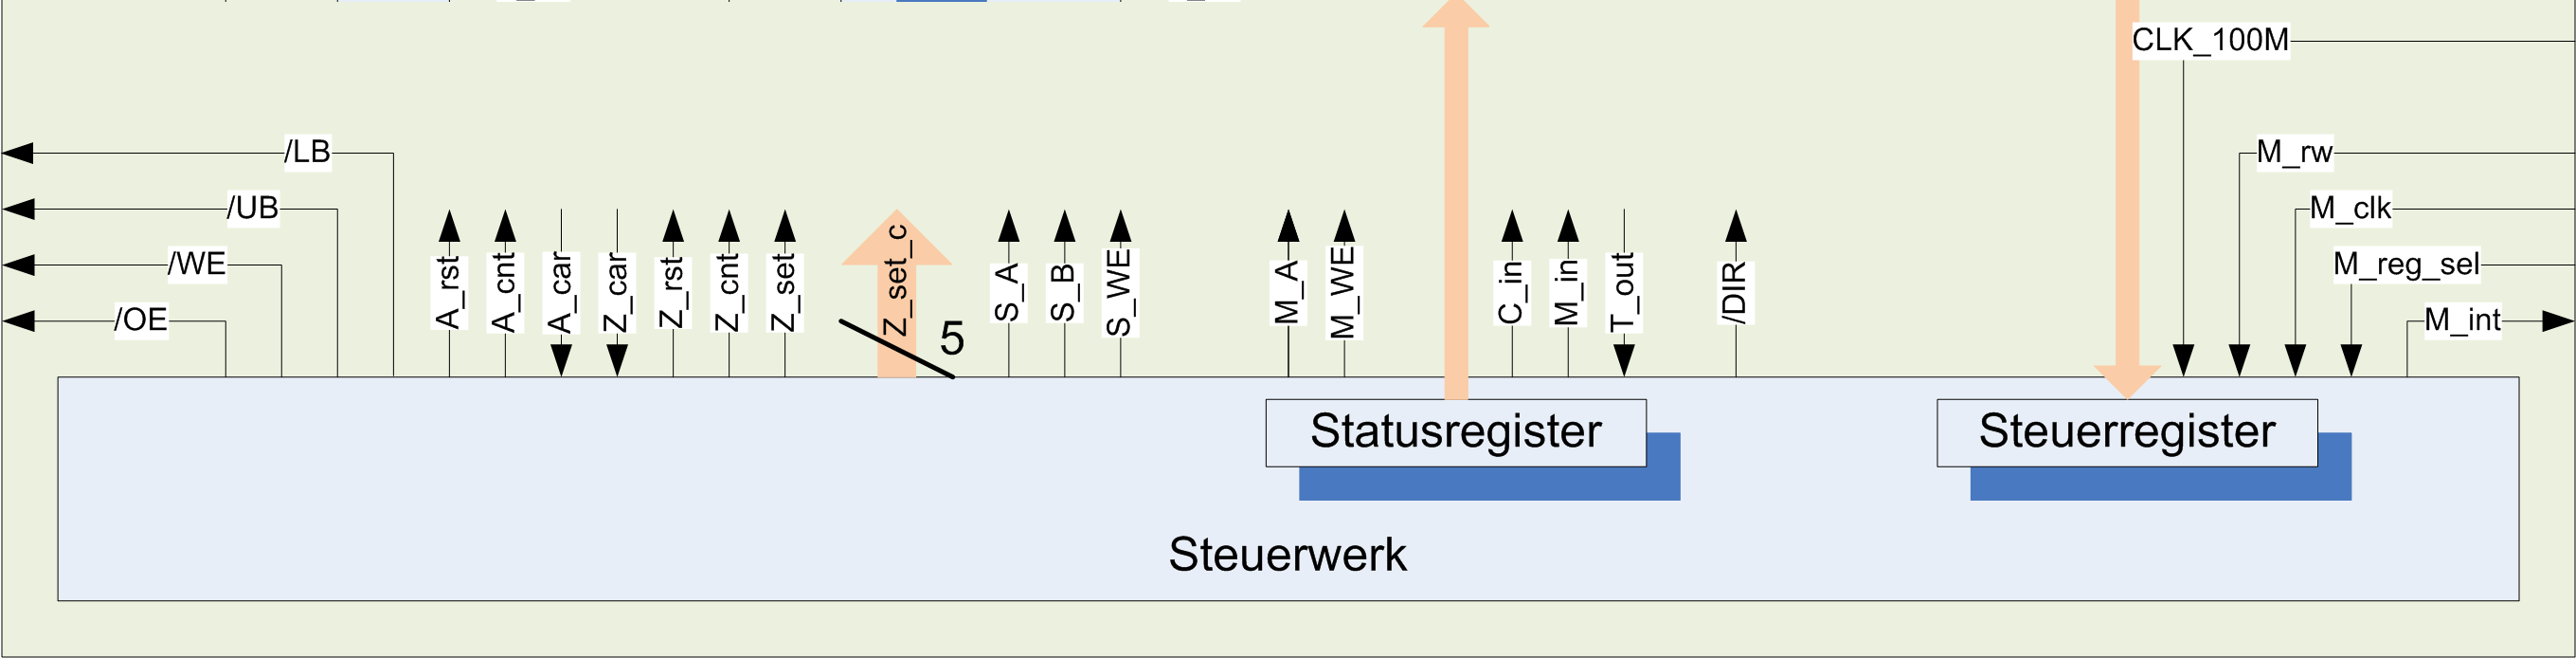
\includegraphics[width=1.0\textwidth]{images/Steuerwerk.png}\\
	\rule{\linewidth}{0.5pt}
	\caption{Blockschaltbild Steuerwerk}
	\label{pic:Steuerwerk}
\end{figure}
\chapter{Ausblick} \index{Ausblick}

In dieser Arbeit wurde nun die Basis f�r einen multifunktionelles Ger�t zur Timing-, Protokoll-, Logik- und Eventanalyse von digitalen Signalen geschaffen.

Um nun aus dieser Plattform ein voll funktionsf�higes Ger�t zu erstellen, m�ssen noch folgende Arbeiten erledigt werden.

\begin{description} 
 \item[USB-Schnittstelle:] F�r die in Kapitel \ref{USB-Schnittstelle} erl�uterte USB-Schnittstelle muss noch die Konfiguration des Logibausteins fertig implementiert werden. F�r Windows-Systeme sollte noch eine .inf-Datei erzeugt werden, um eine problemlose Integration zu erm�glichen.
 \item[Mikrocontroller-Software:] Hier muss die Kommunikationsschnittstelle mit dem CPLD sowie die Aufbereitung der Messdaten implementiert werden. Siehe Kapitel \ref{Mikrocontroller_Software}.
 \item[VHDL-Design:] Das in Kapitel \ref{VHDL-Design} beschriebene VHDL-Design kann auf Basis der bereits erzeugten Quartus-II-Projektdateien implementiert werden.
 \item[PC-Software] Es k�nnte auch eine grafische Bedieneroberfl�che (GUI) erzeugt werden. Dadurch l�sst sich der Analysator nicht nur �ber ein Text-Terminal, sondern auch komfortabel mit der Maus bedienen. Hier k�nnte auch die graphische Anzeige der Messwerte mit integriert werden.
 \end{description}

Diese Arbeiten k�nnen nun, zum Beispiel durch eine Projektkruppe im Rahmen der technischen Projektarbeit oder in einer Abschlussarbeit durchgef�hrt werden.

Durch die sehr flexible Kombination aus Mikrocontroller mit USB-Schnittstelle, Logikbaustein und Speicher, sind allerdings auch viele andere Projekte auf dieser Hardwarebasis denkbar.

\chapter{Anhang}

\section{Schaltplan und Platinenlayout}

\begin{figure}[ht]
	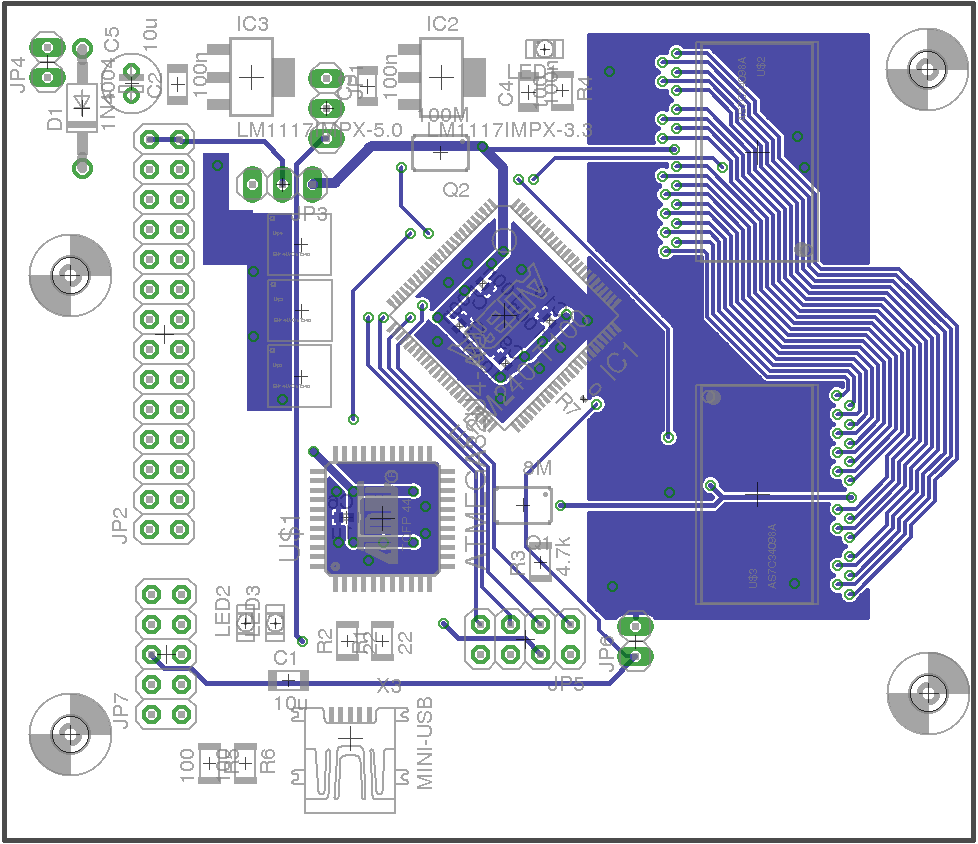
\includegraphics[width=1.0\textwidth]{images/Platine_bot.png}\\
	\rule{\linewidth}{0.5pt}
	\caption{Platinenlayout, Unterseite}
\end{figure}

\begin{figure}[ht]
	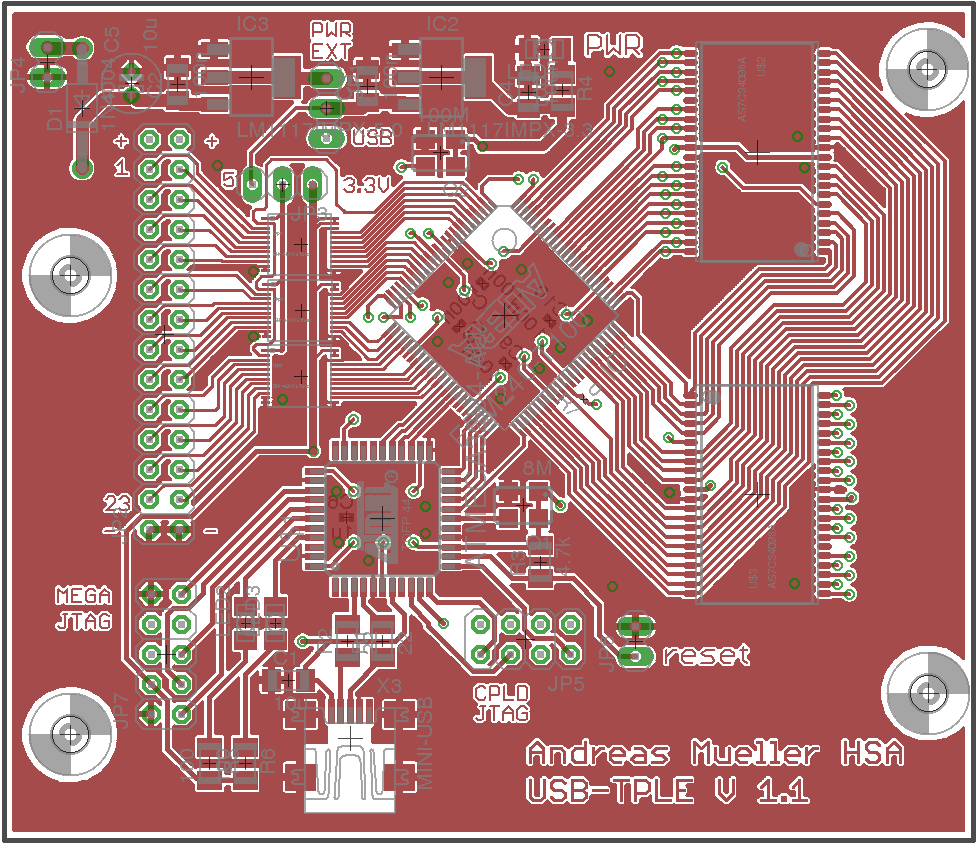
\includegraphics[width=1.0\textwidth]{images/Platine_top.png}\\
	\rule{\linewidth}{0.5pt}
	\caption{Platinenlayout, Oberseite}
\end{figure}

\begin{landscape}
%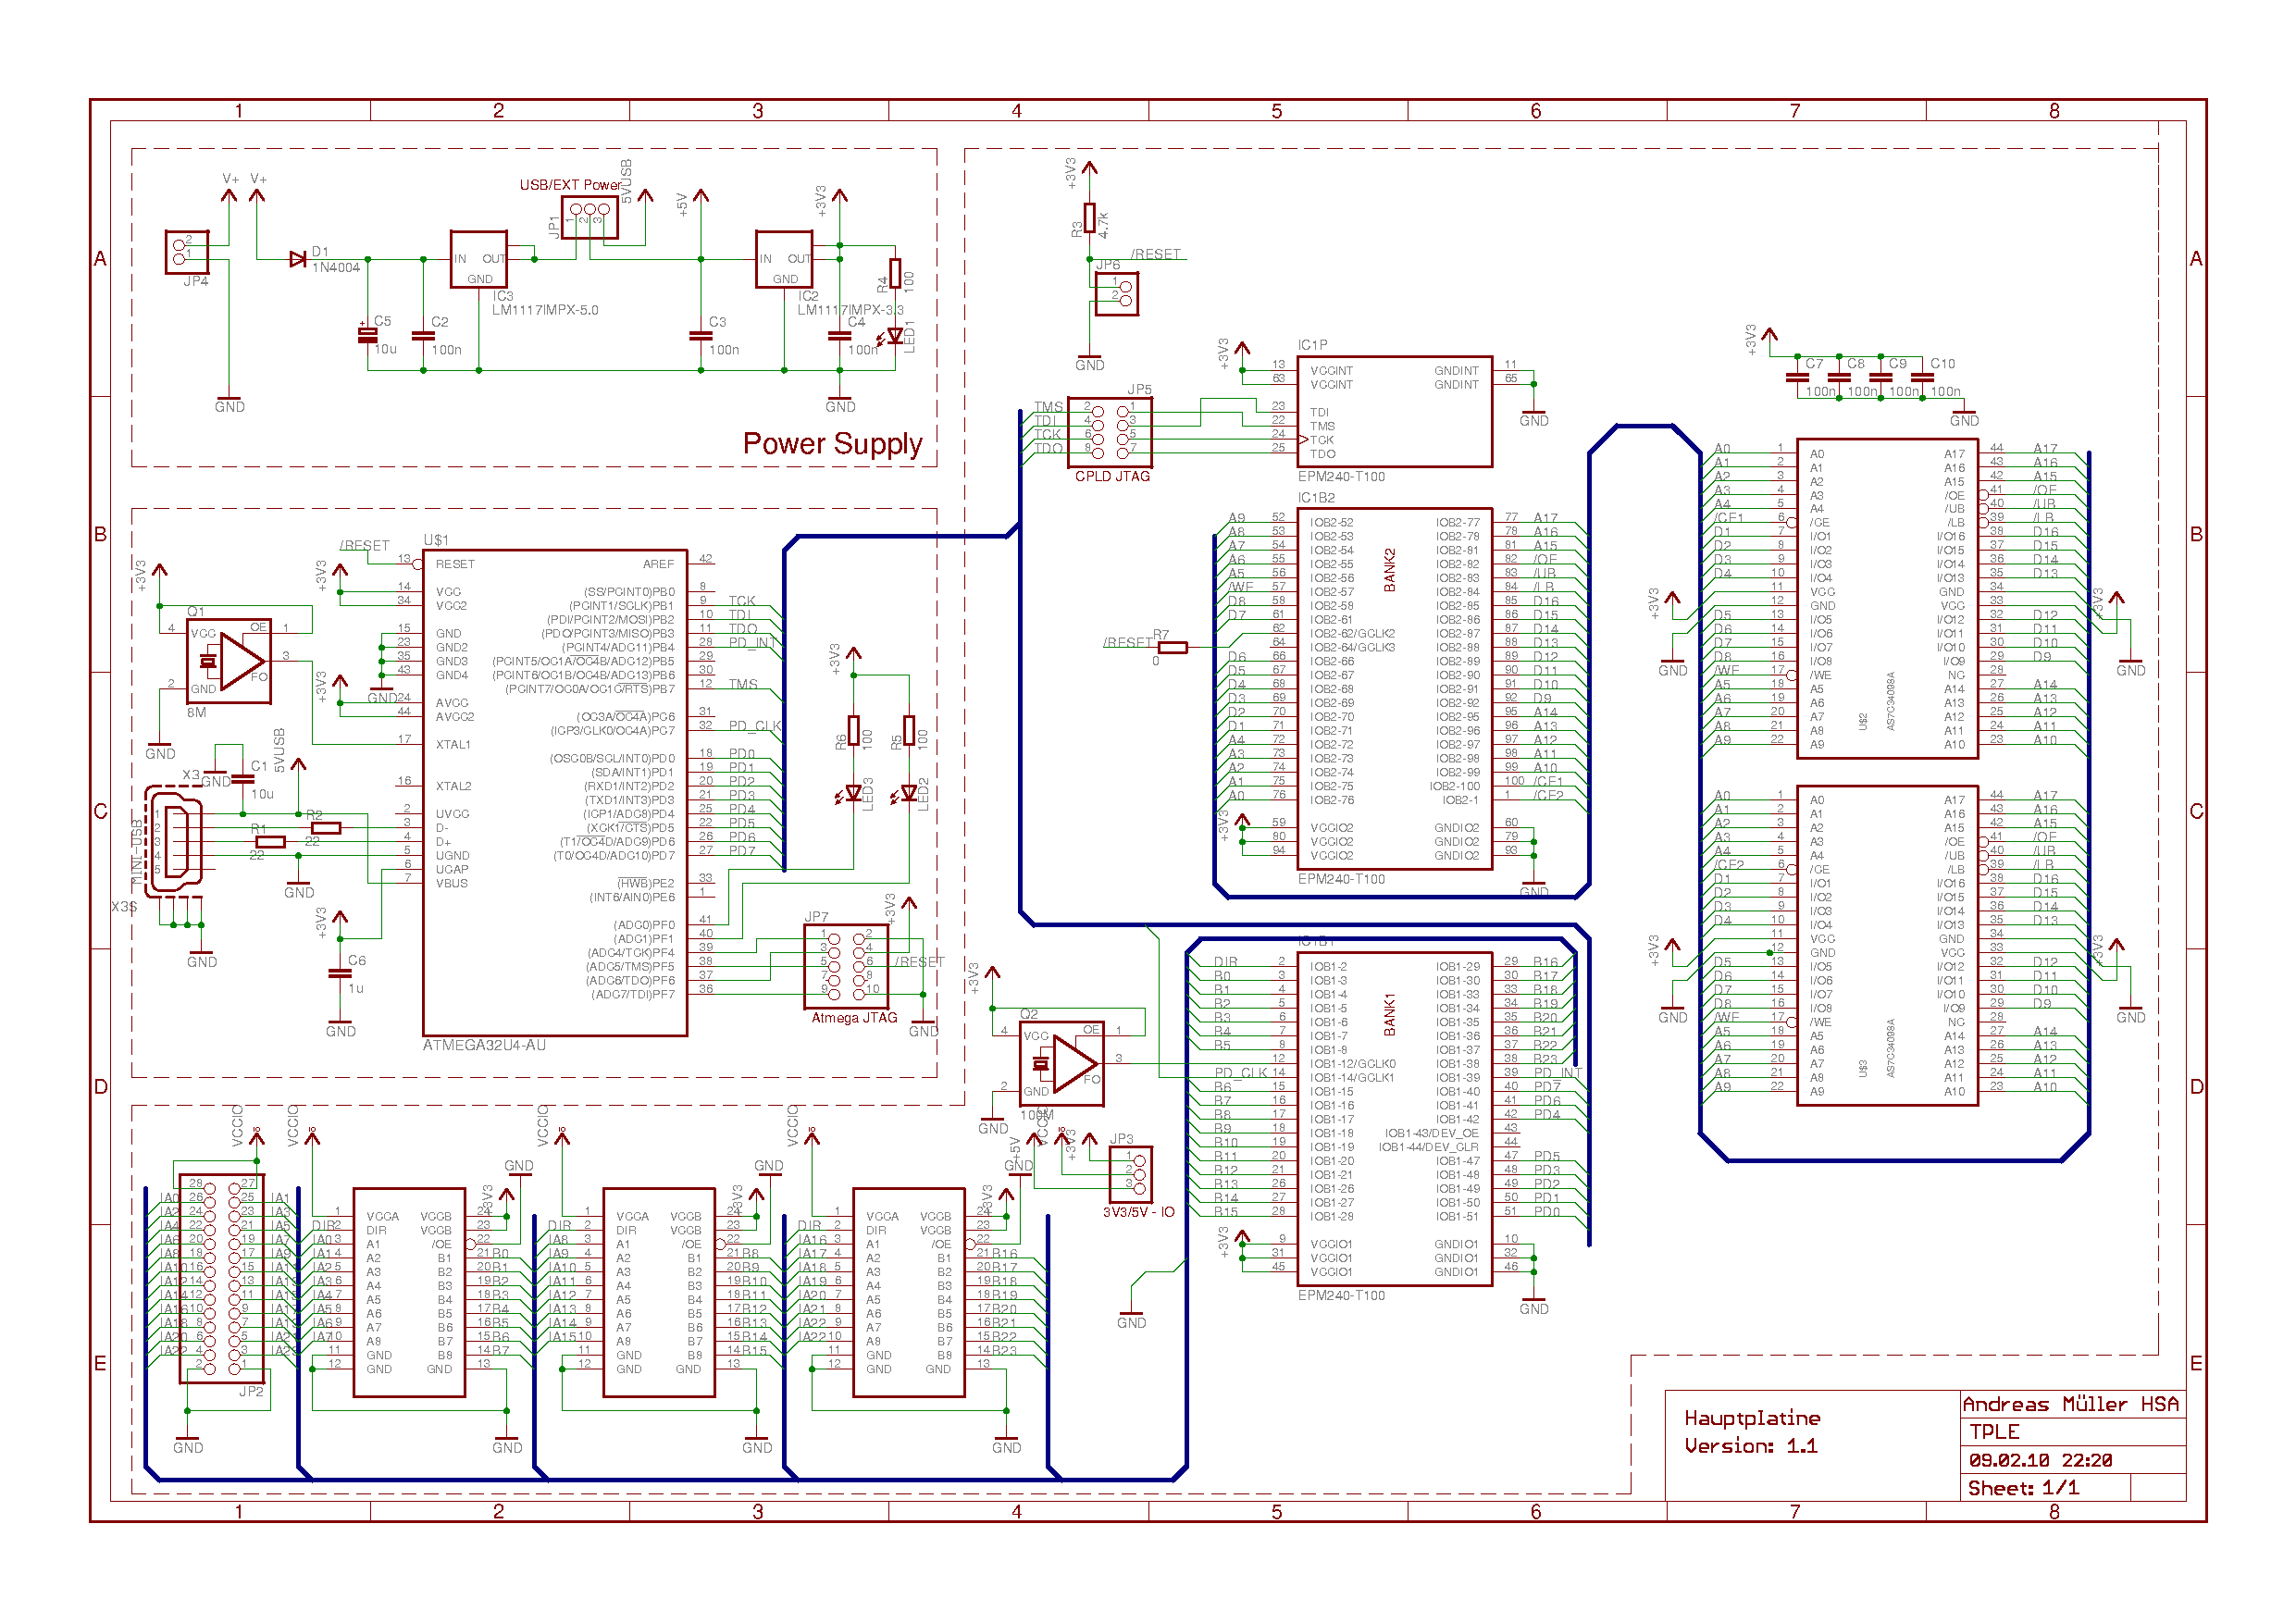
\includepdf{images/main_cirquit_v1_1.pdf}
%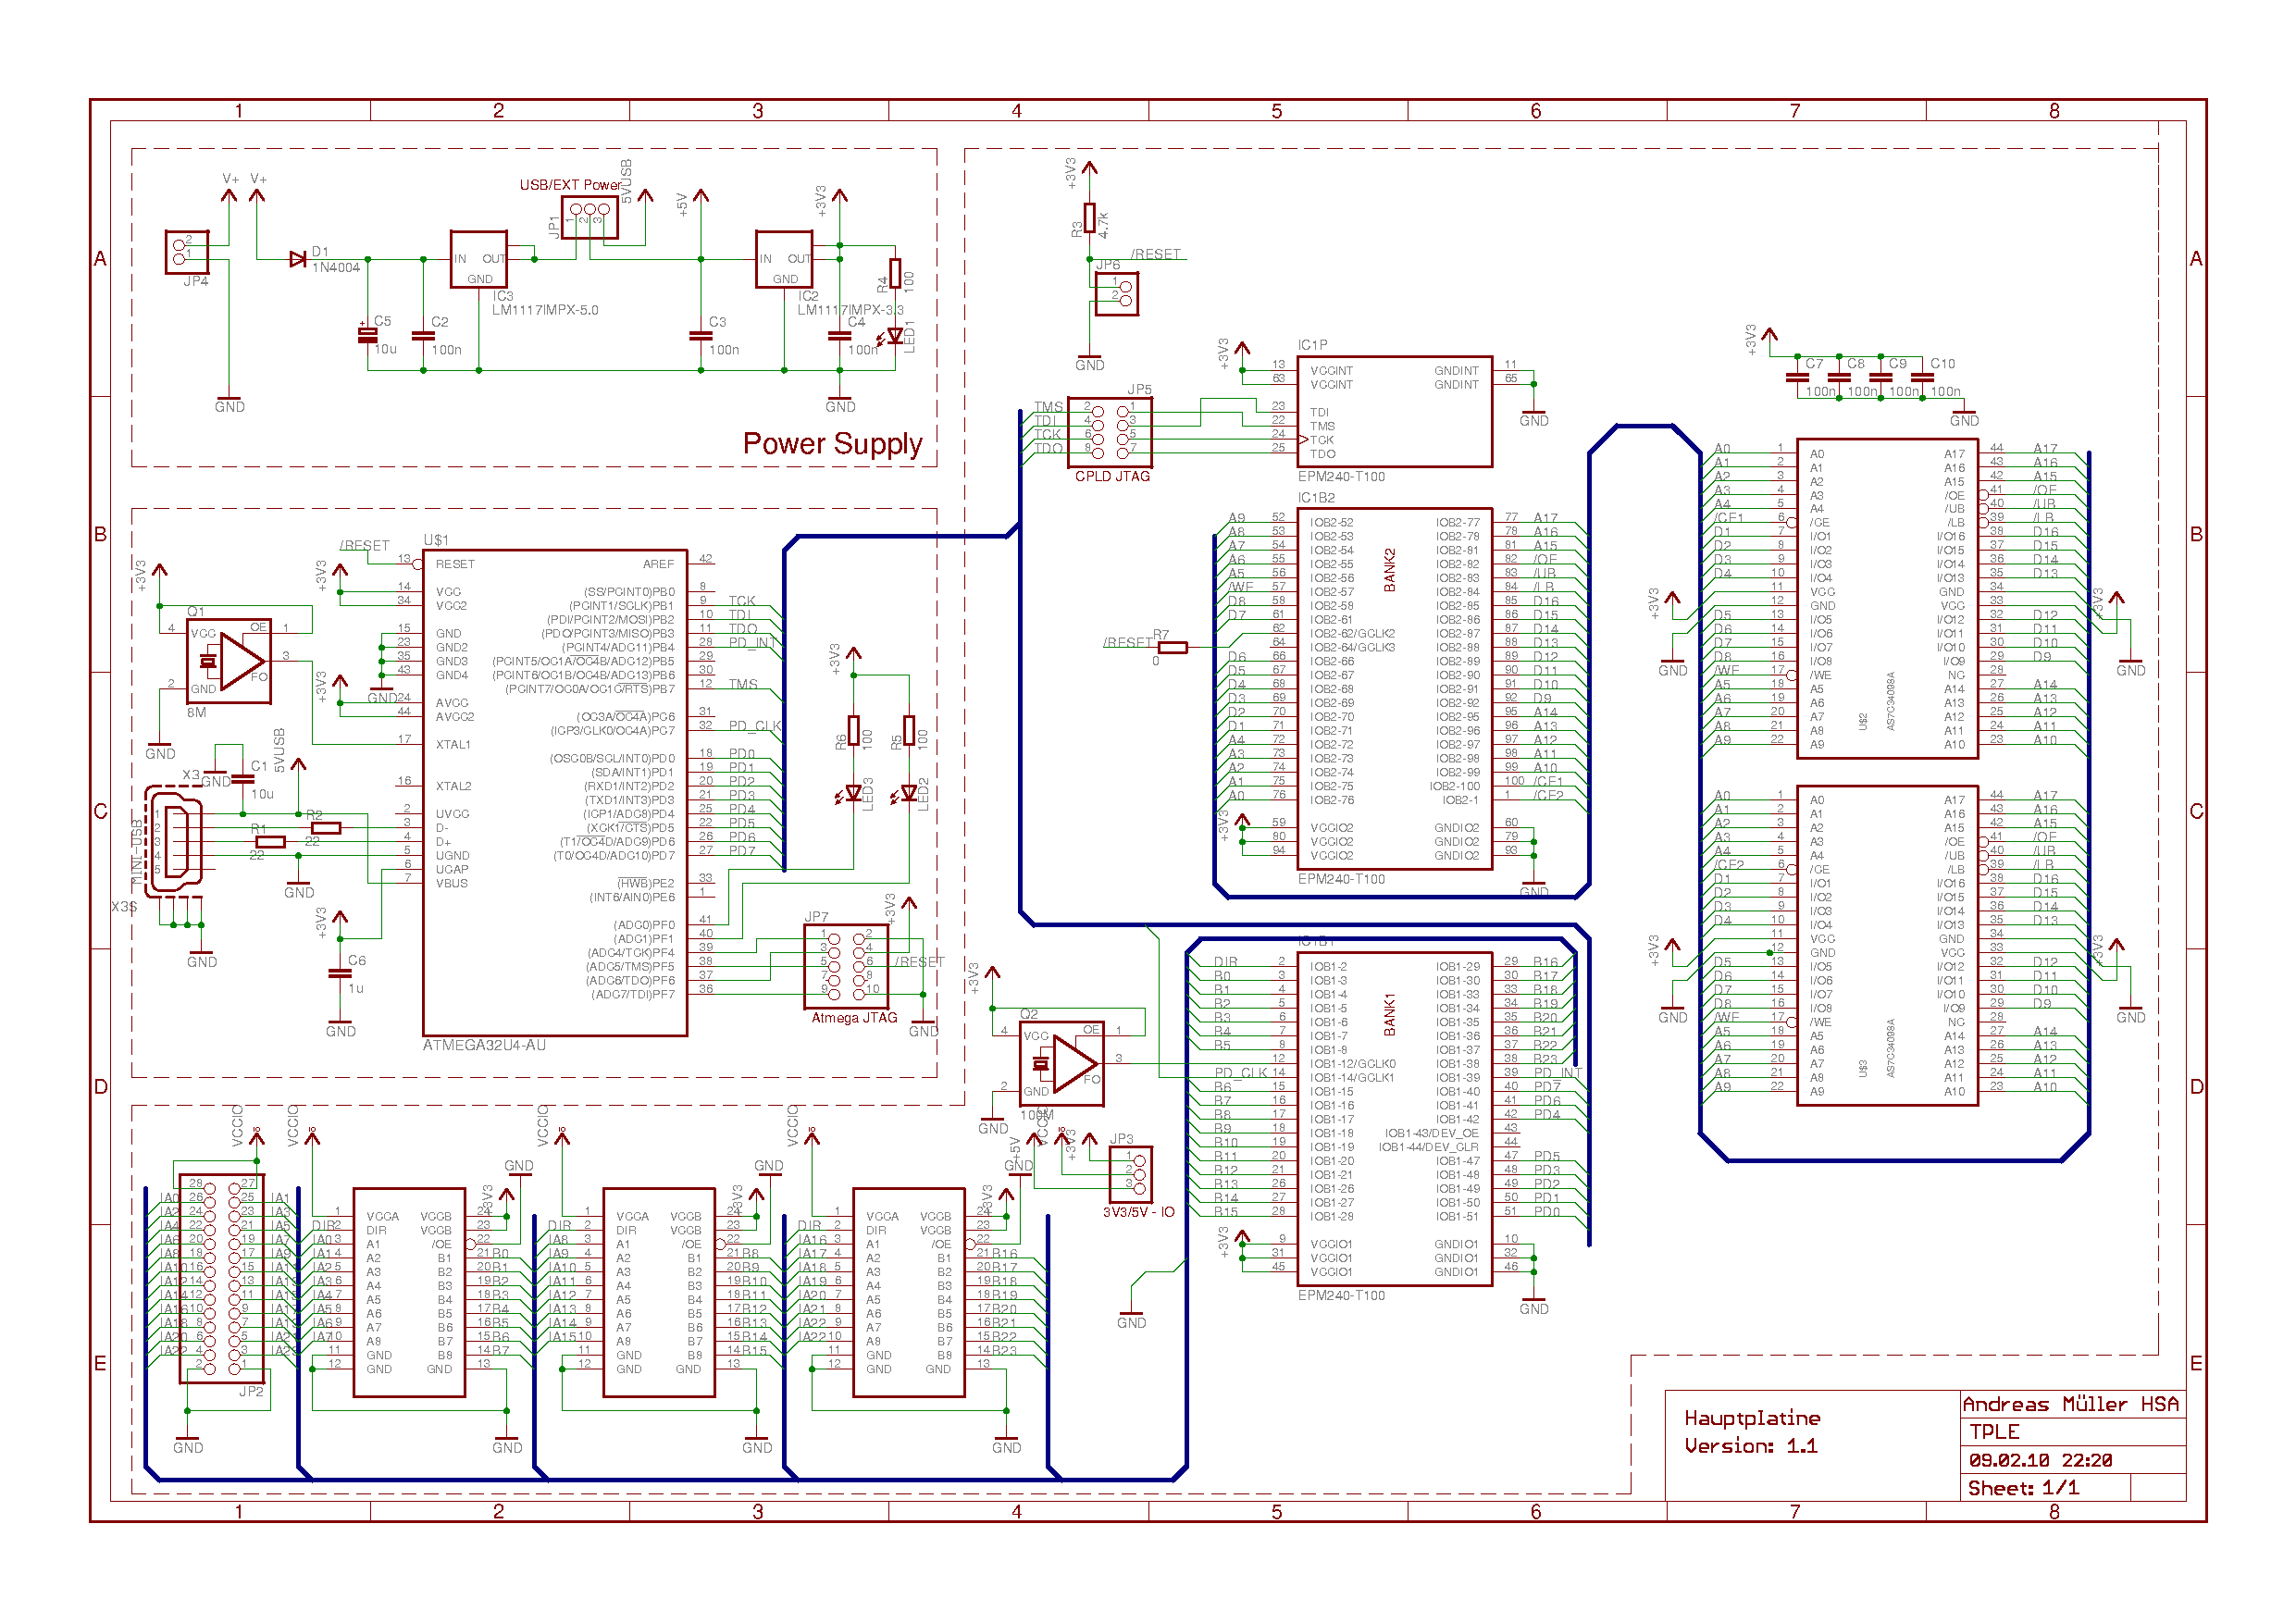
\includegraphics{images/main_cirquit_v1_1.pdf}
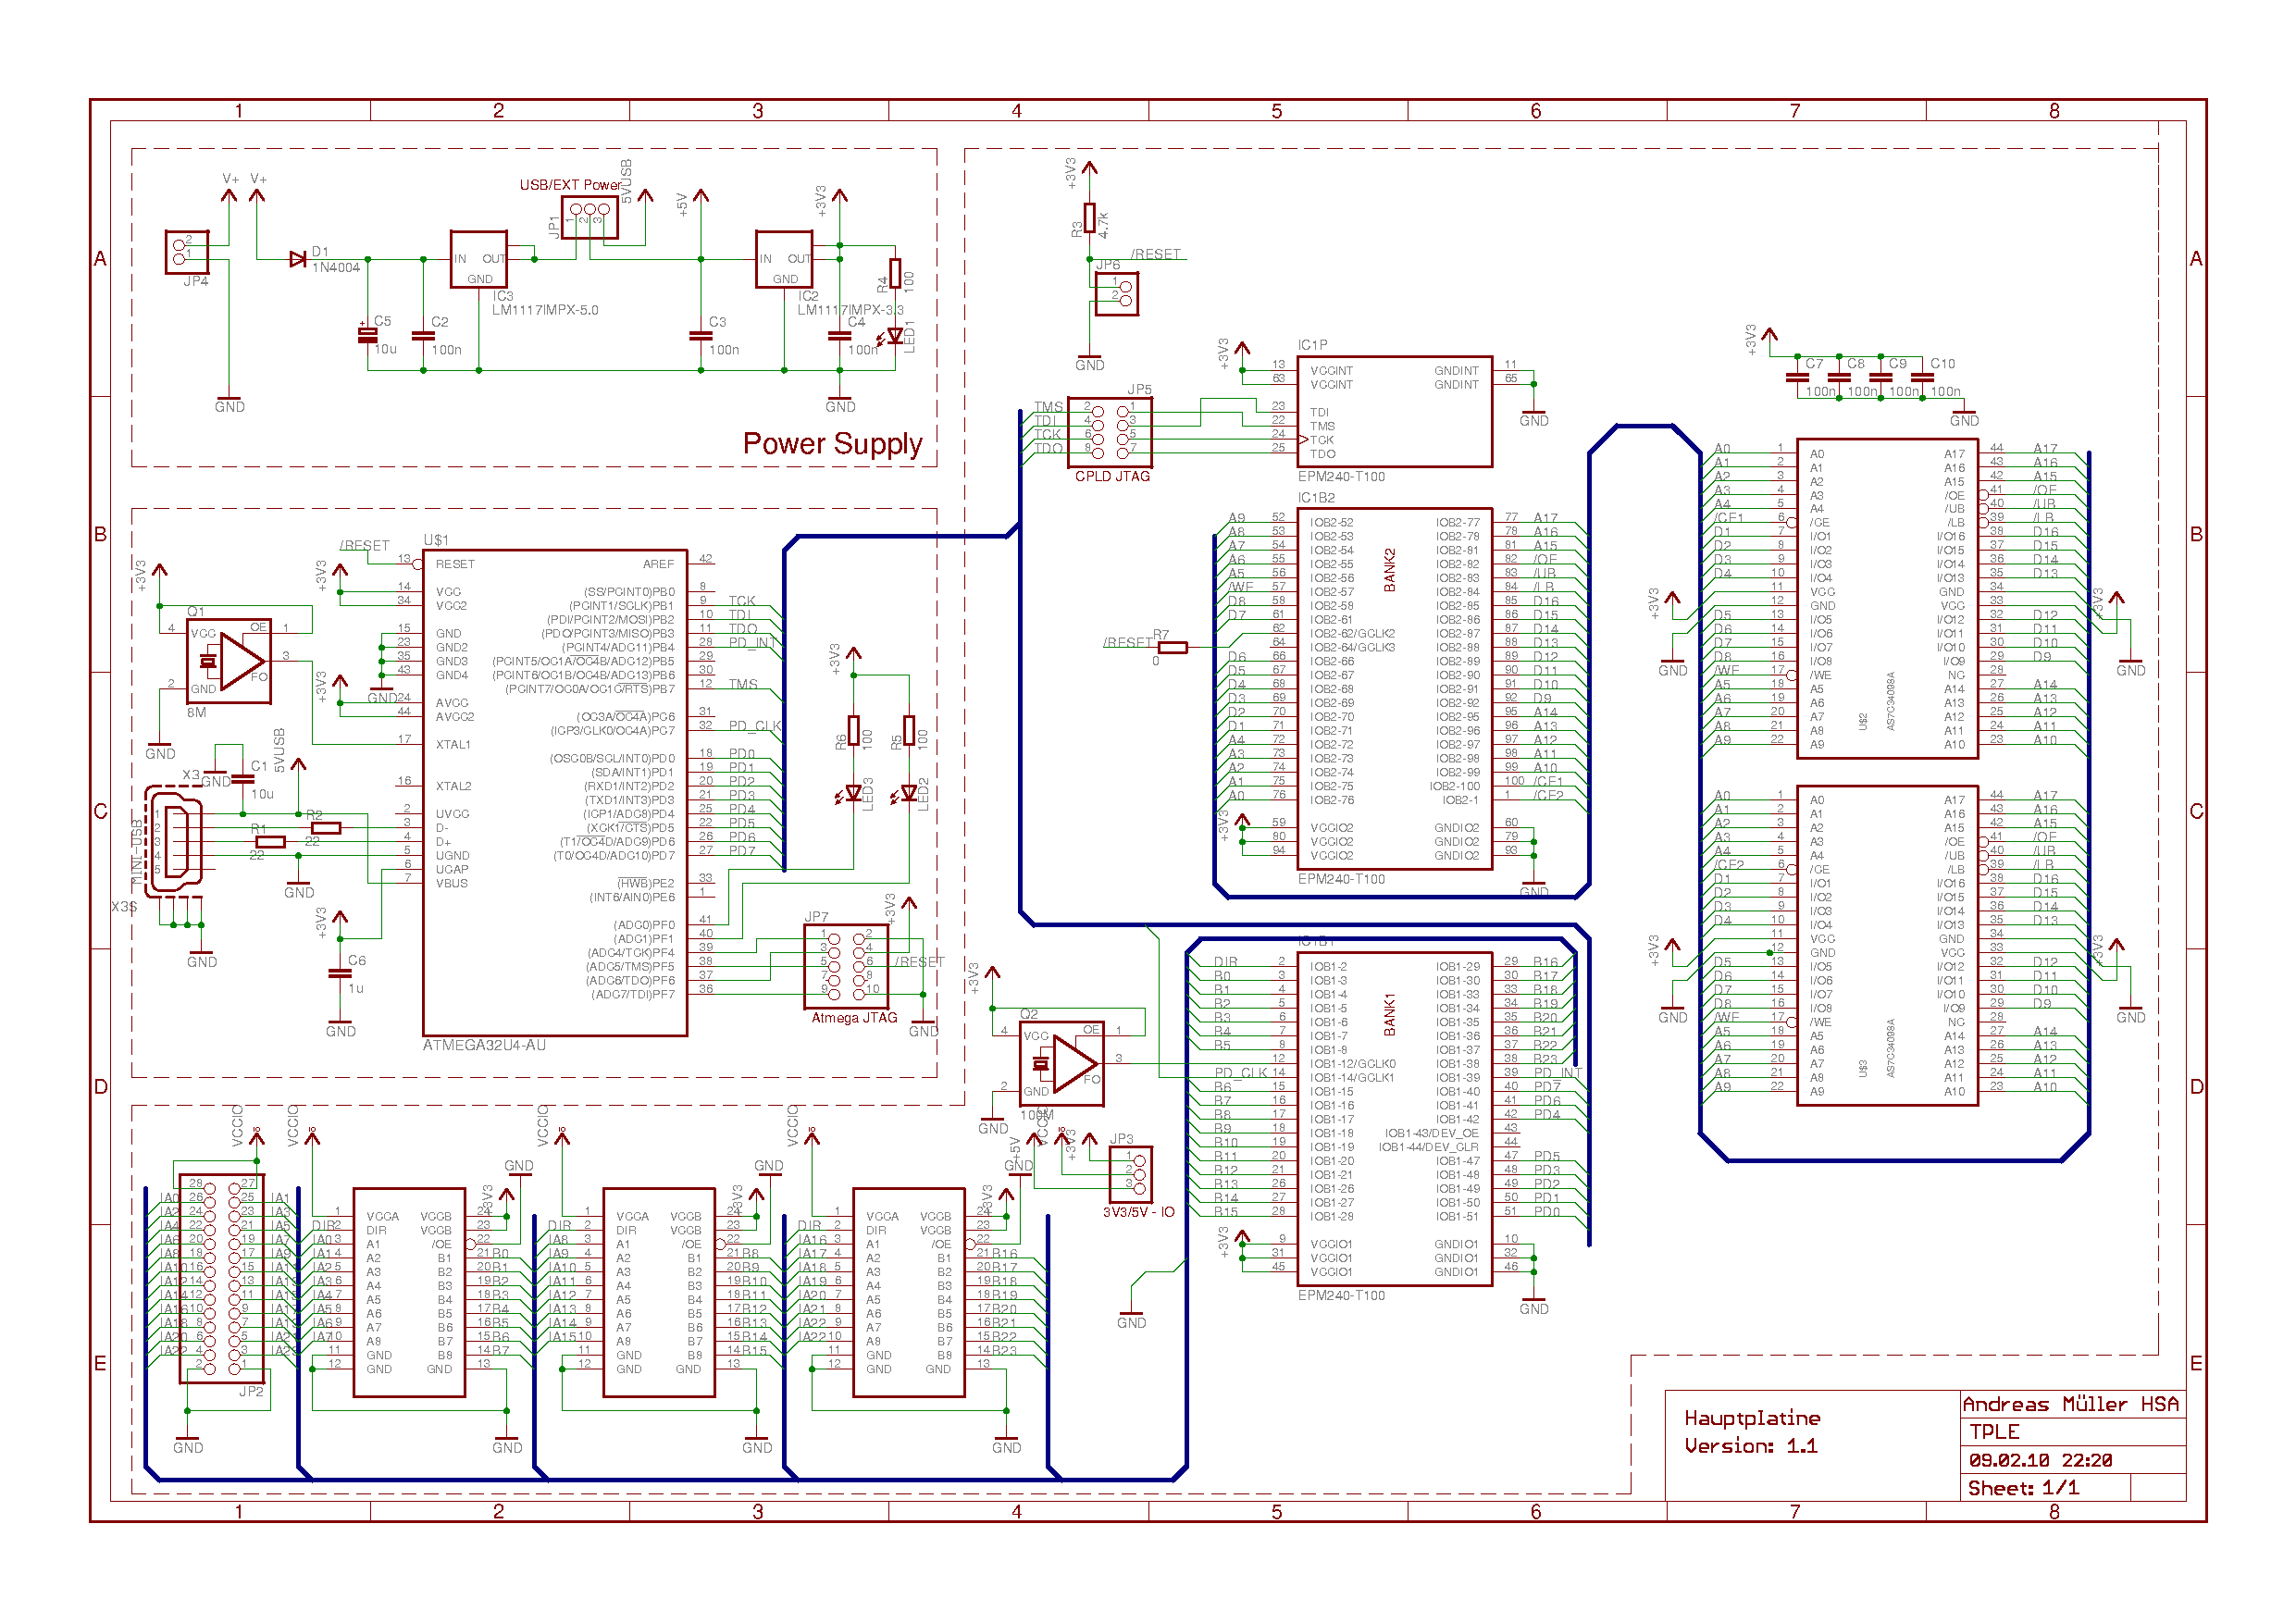
\includegraphics[width=1.4\textwidth]{images/main_cirquit_v1_1.pdf}
\end{landscape}

\section{Bauteile}

\begin{table}[h] 
\begin{tabular}{|l|l|l|l|l|}
\hline
Menge	& Wert		& Bezeichnung		& Bauteilname		& Farnell Bestellnummer \\
\hline \hline
2	& 1X2		& PINHEAD		& JP4, JP6		& ------- \\
2	& 1X3		& PINHEAD		& JP1, JP3 		& ------- \\
1 	& 2X4		& PINHEAD		& JP5			& ------- \\
1	& 2X5		& PINHEAD		& JP7			& ------- \\
1	& 2X14		& PINHEAD		& JP2			& ------- \\
1	& 		& MINI-USB		& X3			& 1558179 \\
2	& 22		& R3216			& R1, R2		& 1577421 \\
1	& 4.7k		& R3216			& R3			& 1717749 \\
3	& 100		& R3216			& R4, R5, R6		& 1717738 \\
1	& 0		& R0201			& R7			& ------- \\
1	& 10u		& C3216			& C1			& 1432339 \\
3	& 100n		& C1206			& C2, C3, C4		& 1759312 \\
1	& 10u		& CPOL2-5		& C5			& ------- \\
1	& 1u		& C0402			& C6			& 1611915 \\
4	& 100n		& C0402			& C7, C8, C9, C10	& 1611916 \\
1	& 1N4004	& Diode			& D1			& 9556109 \\
1	& 8M		& Oszilator		& Q1			& ------- \\
1	& 100M		& Oszilator		& Q2			& 1538960 \\
3	& RED		& LED1206		& LED1, LED2, LED3	& 1318261 \\
1	& ATMEGA32U4-AU	& Microcontroller	& U\$1			& ------- \\
2 	& AS7C34098A	& Memory		& U\$2, U\$3		& 1562920 \\
1	& EPM240-T100	& Altera CPLD		& IC1			& 1453502 \\
1	& LM1117IMPX-3.3 & Regulator		& IC2			& 1652313 \\
1     	& LM1117IMPX-5.0 & Regulator		& IC3			& 1652314 \\
3	& SN74LVC8T245	& BUS-Driver		& U\$4, U\$5, U\$6	& 1236406 \\
\hline
\end{tabular}
\caption{Liste aller n�tigen Bauteile mit Bestellnummern (Falls vorhanden)}
\label{tab:Bauteile}
\end{table}

\newpage

\section{Inhaltsverzeichnis Datentr�ger}

\begin{table}[h] 
\begin{tabular}{|l|l|}
\hline
Verzeichnis						& Beschreibung	\\
\hline \hline
./							& Wurzelverzeichnis \\
./PLD\_Firmware						& Firmware Logikbaustein \\
./PLD\_Firmware/src					& VHDL-Quellcode \\
./PLD\_Firmware/Quartus\_project			& Quartus-II Projektdateien \\
./Microcontroller\_Firmware				& Firmware Mikrocontroller \\
./Microcontroller\_Firmware/LUFA\_Based			& Quellcode Verzeichnis f�r Lufa-Basierenden Quellcode \\
./Microcontroller\_Firmware/LUFA\_Based/estick\_firmware & Estick-JTAG Adapter \\
./Microcontroller\_Firmware/LUFA\_Based/DualSerial	& Duale virtuelle serielle Schnittstelle \\
./Microcontroller\_Firmware/Atmel\_Based		& Quellcode Verzeichnis f�r Lufa-Basierenden Quellcode \\
./Microcontroller\_Firmware/Atmel\_Based/USB\_JTAG\_UART& Jam-Player basierender JTAG-Adapter \\
./Microcontroller\_Firmware/Atmel\_Based/Bootloader	& Atmel Bootloader \\
./Datasheets						& Datenbl�tter \\
./Hardware						& Verzeichnis f�r Schaltpl�ne und Boardlayouts \\
./Hardware/V1.1						& Hardware Revision 1.1 \\
./Hardware/eagle\_lib					& Nicht-Stadard Eagle Bibliotheken \\
./Hardware/V1.0						& Hardware Revision 1.0 \\
./Documentation						& Dokumentation \\
./PC\_Software						& PC-Software \\
./PC\_Software/urjtag-0.10				& UrJTAG \\
./PC\_Software/DFU\_programmer				& Bootloader PC-Software \\
./PC\_Software/USB\_STAPL\_Player			& Software zur CPLD-Konfiguration \\
\hline
\end{tabular}
\caption{Inhaltsverzeichnis Datentr�ger}
\label{tab:Datentraeger}
\end{table}

\listoffigures

% Literaturverzeichnis soll im Inhaltsverzeichnis auftauchen
\addcontentsline{toc}{section}{Literatruverzeichnis}

\begin{thebibliography}{------} \label{Literaturverzeichnis}

\bibitem[Hoffm02]{Hoffm02}
	J. Hoffmann, W. Trentmannm:
	{\em Praxis der PC-Messtechnik}.
	Hanser, 2002 \\
	ISBN 3-446-21708-8 \\

\bibitem[Schwe97]{Schwe97}
	H. Schwetlick:
	{\em PC-Messtechnik}.
	Vieweg, 1997 \\
	ISBN 3-528-04948-4 \\

\bibitem[Kaink00]{Kaink00}
	B. Kainka:
	{\em Messen, Steuern und Regeln mit USB}.
	Franzis Verlag, 2000 \\
	ISBN 3-7723-5874-8 \\

\bibitem[Atmel01]{Atmel01}
	Atmel:
	{\em Atmega32-U4 Datasheet} \\
	\url{http://www.atmel.com/dyn/resources/prod\_documents/doc7766.pdf}\\
	Rev. Juli 2008 \\

\bibitem[Alter01]{Alter01}
	Altera:
	{\em MAX II Device Handbook} \\
	\url{http://www.altera.com/literature/hb/max2/max2\_mii5v1.pdf}\\
	Rev. August 2009 \\

\bibitem[Xilin01]{Xilin01}
	Xilinx:
	{\em Coolrunner II Data Sheet} \\
	\url{http://www.xilinx.com/support/documentation/data\_sheets/ds090.pdf}\\
	Rev. September 2008 \\

\bibitem[Texas01]{Texas01}
	Texas Instruments:
	{\em SN74LVC8T245 Data Sheet} \\
	\url{http://www.ti.com/lit/gpn/sn74lvc8t245}\\
	Rev. Juni 2005 \\ 

\bibitem[Allia01]{Allia01}
	Alliance Memory:
	{\em AS7C34098A Data Sheet} \\
	\url{http://www.alliancememory.com/pdf/sram/fa/as7c34098a\_v2.1.pdf}\\
	Rev. August 2004 \\

\bibitem[Atmel02]{Atmel02}
	Atmel:
	{\em AVE329: USB Firmware Archtecture} \\
	\url{http://www.atmel.com/dyn/resources/prod\_documents/doc7703.pdf}\\
	Rev. Februar 2006 \\

\bibitem[Lufa01]{Lufa01}
	Lufa Homepage \\
	\url{http://www.fourwalledcubicle.com/index.php}\\
	Rev. 13. Mai 2010 \\

\bibitem[Alter02]{Alter02}
	Altera:
	{\em Using Jam STAPL for ISP via an Embedded Processor} \\
	\url{http://www.altera.com/literature/hb/max2/max2\_mii51015.pdf}\\
	Rev. Oktober 2008 \\

\bibitem[Khirm01]{Khirm01}
	Stas Khirman:
	{\em JTAG FAQ} \\
	\url{http://hri.sourceforge.net/tools/jtag\_faq\_org.html}\\
	Rev. Februar 2004 \\

\bibitem[IEEE001]{IEEE001}
	IEEE-Standard:
	{\em 1364-2001} \\
	\url{http://ieeexplore.ieee.org/xpls/abs\_all.jsp?arnumber=954909}\\
	Rev. Februar 2004 \\



\end{thebibliography}


\renewcommand{\labelenumii}{\alph{enumii})}
\renewcommand{\labelenumiii}{\arabic{enumiii})}

\chapter{GNU Lesser General Public License}

%\begin{LARGE} GNU LESSER GENERAL PUBLIC LICENSE \end{LARGE} \\
\begin{Large}Version 3, 29 June 2007\end{Large} \\


\begin{center}
{\parindent 0in

Copyright \copyright\  2007 Free Software Foundation, Inc. \texttt{http://fsf.org/}

\bigskip
Everyone is permitted to copy and distribute verbatim copies of this

license document, but changing it is not allowed.}

\end{center}


  This version of the GNU Lesser General Public License incorporates
the terms and conditions of version 3 of the GNU General Public
License, supplemented by the additional permissions listed below.

\begin{enumerate}
\addtocounter{enumi}{-1}  % start at 0

\item Additional Definitions.

  As used herein, ``this License'' refers to version 3 of the GNU Lesser
General Public License, and the ``GNU GPL'' refers to version 3 of the GNU
General Public License.

  ``The Library'' refers to a covered work governed by this License,
other than an Application or a Combined Work as defined below.

  An ``Application'' is any work that makes use of an interface provided
by the Library, but which is not otherwise based on the Library.
Defining a subclass of a class defined by the Library is deemed a mode
of using an interface provided by the Library.

  A ``Combined Work'' is a work produced by combining or linking an
Application with the Library.  The particular version of the Library
with which the Combined Work was made is also called the ``Linked
Version''.

  The ``Minimal Corresponding Source'' for a Combined Work means the
Corresponding Source for the Combined Work, excluding any source code
for portions of the Combined Work that, considered in isolation, are
based on the Application, and not on the Linked Version.

  The ``Corresponding Application Code'' for a Combined Work means the
object code and/or source code for the Application, including any data
and utility programs needed for reproducing the Combined Work from the
Application, but excluding the System Libraries of the Combined Work.

\item Exception to Section 3 of the GNU GPL.

  You may convey a covered work under sections 3 and 4 of this License
without being bound by section 3 of the GNU GPL.

\item Conveying Modified Versions.

  If you modify a copy of the Library, and, in your modifications, a
facility refers to a function or data to be supplied by an Application
that uses the facility (other than as an argument passed when the
facility is invoked), then you may convey a copy of the modified
version:

   \begin{enumerate}
   \item under this License, provided that you make a good faith effort to
   ensure that, in the event an Application does not supply the
   function or data, the facility still operates, and performs
   whatever part of its purpose remains meaningful, or

   \item under the GNU GPL, with none of the additional permissions of
   this License applicable to that copy.
   \end{enumerate}

\item Object Code Incorporating Material from Library Header Files.

  The object code form of an Application may incorporate material from
a header file that is part of the Library.  You may convey such object
code under terms of your choice, provided that, if the incorporated
material is not limited to numerical parameters, data structure
layouts and accessors, or small macros, inline functions and templates
(ten or fewer lines in length), you do both of the following:

   \begin{enumerate}
   \item Give prominent notice with each copy of the object code that the
   Library is used in it and that the Library and its use are
   covered by this License.

   \item Accompany the object code with a copy of the GNU GPL and this license
   document.
   \end{enumerate}

\item Combined Works.

  You may convey a Combined Work under terms of your choice that,
taken together, effectively do not restrict modification of the
portions of the Library contained in the Combined Work and reverse
engineering for debugging such modifications, if you also do each of
the following:

   \begin{enumerate}
   \item Give prominent notice with each copy of the Combined Work that
   the Library is used in it and that the Library and its use are
   covered by this License.

   \item Accompany the Combined Work with a copy of the GNU GPL and this license
   document.

   \item For a Combined Work that displays copyright notices during
   execution, include the copyright notice for the Library among
   these notices, as well as a reference directing the user to the
   copies of the GNU GPL and this license document.

   \item Do one of the following:

       \begin{enumerate}
       \addtocounter{enumiii}{-1}  % start at 0
       \item Convey the Minimal Corresponding Source under the terms of this
       License, and the Corresponding Application Code in a form
       suitable for, and under terms that permit, the user to
       recombine or relink the Application with a modified version of
       the Linked Version to produce a modified Combined Work, in the
       manner specified by section 6 of the GNU GPL for conveying
       Corresponding Source.

       \item Use a suitable shared library mechanism for linking with the
       Library.  A suitable mechanism is one that (a) uses at run time
       a copy of the Library already present on the user's computer
       system, and (b) will operate properly with a modified version
       of the Library that is interface-compatible with the Linked
       Version. 
       \end{enumerate}

   \item Provide Installation Information, but only if you would otherwise
   be required to provide such information under section 6 of the
   GNU GPL, and only to the extent that such information is
   necessary to install and execute a modified version of the
   Combined Work produced by recombining or relinking the
   Application with a modified version of the Linked Version. (If
   you use option 4d0, the Installation Information must accompany
   the Minimal Corresponding Source and Corresponding Application
   Code. If you use option 4d1, you must provide the Installation
   Information in the manner specified by section 6 of the GNU GPL
   for conveying Corresponding Source.)
   \end{enumerate}

\item Combined Libraries.

  You may place library facilities that are a work based on the
Library side by side in a single library together with other library
facilities that are not Applications and are not covered by this
License, and convey such a combined library under terms of your
choice, if you do both of the following:

   \begin{enumerate}
   \item Accompany the combined library with a copy of the same work based
   on the Library, uncombined with any other library facilities,
   conveyed under the terms of this License.

   \item Give prominent notice with the combined library that part of it
   is a work based on the Library, and explaining where to find the
   accompanying uncombined form of the same work.
   \end{enumerate}

\item Revised Versions of the GNU Lesser General Public License.

  The Free Software Foundation may publish revised and/or new versions
of the GNU Lesser General Public License from time to time. Such new
versions will be similar in spirit to the present version, but may
differ in detail to address new problems or concerns.

  Each version is given a distinguishing version number. If the
Library as you received it specifies that a certain numbered version
of the GNU Lesser General Public License ``or any later version''
applies to it, you have the option of following the terms and
conditions either of that published version or of any later version
published by the Free Software Foundation. If the Library as you
received it does not specify a version number of the GNU Lesser
General Public License, you may choose any version of the GNU Lesser
General Public License ever published by the Free Software Foundation.

  If the Library as you received it specifies that a proxy can decide
whether future versions of the GNU Lesser General Public License shall
apply, that proxy's public statement of acceptance of any version is
permanent authorization for you to choose that version for the
Library.

\end{enumerate}

\printindex


\end{document}